% **************************************************************************************************************
% A Classic Thesis Style
% An Homage to The Elements of Typographic Style
%
% Copyright (C) 2018 André Miede and Ivo Pletikosić
%
% If you like the style then I would appreciate a postcard. My address
% can be found in the file ClassicThesis.pdf. A collection of the
% postcards I received so far is available online at
% http://postcards.miede.de
%
% License:
% This program is free software; you can redistribute it and/or modify
% it under the terms of the GNU General Public License as published by
% the Free Software Foundation; either version 2 of the License, or
% (at your option) any later version.
%
% This program is distributed in the hope that it will be useful,
% but WITHOUT ANY WARRANTY; without even the implied warranty of
% MERCHANTABILITY or FITNESS FOR A PARTICULAR PURPOSE.  See the
% GNU General Public License for more details.
%
% You should have received a copy of the GNU General Public License
% along with this program; see the file COPYING.  If not, write to
% the Free Software Foundation, Inc., 59 Temple Place - Suite 330,
% Boston, MA 02111-1307, USA.
%
% PLEASE SEE ALSO THE AUTHORS' NOTE REGARDING THIS LICENSE
% IN THE DOCUMENTATION (ClassicThesis.pdf --> Chapter 1 / Chapter01.tex)
% **************************************************************************************************************
\RequirePackage{silence} % :-\
    \WarningFilter{scrreprt}{Usage of package `titlesec'}
    %\WarningFilter{scrreprt}{Activating an ugly workaround}
    \WarningFilter{titlesec}{Non standard sectioning command detected}
\documentclass[ twoside,openright,titlepage,numbers=noenddot,%1headlines,
                headinclude,footinclude,cleardoublepage=empty,abstract=on,
                BCOR=5mm,paper=a4,fontsize=12pt
                ]{scrreprt}

%********************************************************************
% Note: Make all your adjustments in here
%*******************************************************
% ****************************************************************************************************
% classicthesis-config.tex
% formerly known as loadpackages.sty, classicthesis-ldpkg.sty, and classicthesis-preamble.sty
% Use it at the beginning of your ClassicThesis.tex, or as a LaTeX Preamble
% in your ClassicThesis.{tex,lyx} with % ****************************************************************************************************
% classicthesis-config.tex
% formerly known as loadpackages.sty, classicthesis-ldpkg.sty, and classicthesis-preamble.sty
% Use it at the beginning of your ClassicThesis.tex, or as a LaTeX Preamble
% in your ClassicThesis.{tex,lyx} with % ****************************************************************************************************
% classicthesis-config.tex
% formerly known as loadpackages.sty, classicthesis-ldpkg.sty, and classicthesis-preamble.sty
% Use it at the beginning of your ClassicThesis.tex, or as a LaTeX Preamble
% in your ClassicThesis.{tex,lyx} with \input{classicthesis-config}
% ****************************************************************************************************
% If you like the classicthesis, then I would appreciate a postcard.
% My address can be found in the file ClassicThesis.pdf. A collection
% of the postcards I received so far is available online at
% http://postcards.miede.de
% ****************************************************************************************************


% ****************************************************************************************************
% 0. Set the encoding of your files. UTF-8 is the only sensible encoding nowadays. If you can't read
% äöüßáéçèê∂åëæƒÏ€ then change the encoding setting in your editor, not the line below. If your editor
% does not support utf8 use another editor!
% ****************************************************************************************************
\PassOptionsToPackage{utf8}{inputenc}
  \usepackage{inputenc}

\PassOptionsToPackage{T1}{fontenc} % T2A for cyrillics
  \usepackage{fontenc}


% ****************************************************************************************************
% 1. Configure classicthesis for your needs here, e.g., remove "drafting" below
% in order to deactivate the time-stamp on the pages
% (see ClassicThesis.pdf for more information):
% ****************************************************************************************************
\PassOptionsToPackage{
  drafting=false,    % print version information on the bottom of the pages
  tocaligned=false, % the left column of the toc will be aligned (no indentation)
  dottedtoc=false,  % page numbers in ToC flushed right
  eulerchapternumbers=true, % use AMS Euler for chapter font (otherwise Palatino)
  linedheaders=false,       % chaper headers will have line above and beneath
  floatperchapter=true,     % numbering per chapter for all floats (i.e., Figure 1.1)
  eulermath=false,  % use awesome Euler fonts for mathematical formulae (only with pdfLaTeX)
  beramono=true,    % toggle a nice monospaced font (w/ bold)
  palatino=true,    % deactivate standard font for loading another one, see the last section at the end of this file for suggestions
  style=classicthesis % classicthesis, arsclassica
}{classicthesis}


% ****************************************************************************************************
% 2. Personal data and user ad-hoc commands (insert your own data here)
% ****************************************************************************************************
\newcommand{\myTitle}{Goutte soufflée : croissance et dynamique d'une goutte cisaillée par un écoulement d'air\xspace}
\newcommand{\mySubtitle}{Stage de master 2 recherche\xspace}
\newcommand{\myDegree}{Put data \xspace}
\newcommand{\myName}{Guy Raymond BESSENG A IREH\xspace}
\newcommand{\myProf}{Romain MATHIS\xspace}
\newcommand{\myOtherProf}{Julien SEBILLEAU\xspace}
\newcommand{\AnotherProf}{Dominique LEGENDRE\xspace}
\newcommand{\fromUniversity}{Encadrant de l'université\xspace}
\newcommand{\fromLab}{Encadrants du laboratoire IMFT\xspace}
\newcommand{\mySupervisor}{Pierre BRANCHER\xspace}
\newcommand{\myFaculty}{Université Toulouse III - Paul Sabatier\xspace}
\newcommand{\myDepartment}{Département de mécanique\xspace}
\newcommand{\myUni}{Université Toulouse III - Paul Sabatier\xspace}
\newcommand{\myLocation}{Toulouse\xspace}
\newcommand{\myTime}{28 Juin 2018\xspace}
\newcommand{\myVersion}{\classicthesis}

% ********************************************************************
% Setup, finetuning, and useful commands
% ********************************************************************
\providecommand{\mLyX}{L\kern-.1667em\lower.25em\hbox{Y}\kern-.125emX\@}
\newcommand{\ie}{i.\,e.}
\newcommand{\Ie}{I.\,e.}
\newcommand{\eg}{e.\,g.}
\newcommand{\Eg}{E.\,g.}
% ****************************************************************************************************


% ****************************************************************************************************
% 3. Loading some handy packages
% ****************************************************************************************************
% ********************************************************************
% Packages with options that might require adjustments
% ********************************************************************
\PassOptionsToPackage{ngerman,american}{babel} % change this to your language(s), main language last
% Spanish languages need extra options in order to work with this template
%\PassOptionsToPackage{spanish,es-lcroman}{babel}
    \usepackage{babel}

\usepackage{csquotes}
\PassOptionsToPackage{%
  %backend=biber,bibencoding=utf8, %instead of bibtex
  backend=bibtex8,bibencoding=ascii,%
  language=auto,%
  style=numeric-comp,%
  %style=authoryear-comp, % Author 1999, 2010
  %bibstyle=authoryear,dashed=false, % dashed: substitute rep. author with ---
  sorting=nyt, % name, year, title
  maxbibnames=10, % default: 3, et al.
  %backref=true,%
  natbib=true % natbib compatibility mode (\citep and \citet still work)
}{biblatex}
    \usepackage{biblatex}

\PassOptionsToPackage{fleqn}{amsmath}       % math environments and more by the AMS
  \usepackage{amsmath}

% ********************************************************************
% General useful packages
% ********************************************************************
\usepackage{graphicx} %
\usepackage{scrhack} % fix warnings when using KOMA with listings package
\usepackage{xspace} % to get the spacing after macros right
\PassOptionsToPackage{printonlyused,smaller}{acronym}
  \usepackage{acronym} % nice macros for handling all acronyms in the thesis
  %\renewcommand{\bflabel}[1]{{#1}\hfill} % fix the list of acronyms --> no longer working
  %\renewcommand*{\acsfont}[1]{\textsc{#1}}
  %\renewcommand*{\aclabelfont}[1]{\acsfont{#1}}
  %\def\bflabel#1{{#1\hfill}}
  \def\bflabel#1{{\acsfont{#1}\hfill}}
  \def\aclabelfont#1{\acsfont{#1}}
% ****************************************************************************************************
%\usepackage{pgfplots} % External TikZ/PGF support (thanks to Andreas Nautsch)
%\usetikzlibrary{external}
%\tikzexternalize[mode=list and make, prefix=ext-tikz/]
% ****************************************************************************************************


% ****************************************************************************************************
% 4. Setup floats: tables, (sub)figures, and captions
% ****************************************************************************************************
\usepackage{tabularx} % better tables
  \setlength{\extrarowheight}{3pt} % increase table row height
\newcommand{\tableheadline}[1]{\multicolumn{1}{l}{\spacedlowsmallcaps{#1}}}
\newcommand{\myfloatalign}{\centering} % to be used with each float for alignment
\usepackage{subfig}
% ****************************************************************************************************


% ****************************************************************************************************
% 5. Setup code listings
% ****************************************************************************************************
\usepackage{listings}
%\lstset{emph={trueIndex,root},emphstyle=\color{BlueViolet}}%\underbar} % for special keywords
\lstset{language=[LaTeX]Tex,%C++,
  morekeywords={PassOptionsToPackage,selectlanguage},
  keywordstyle=\color{RoyalBlue},%\bfseries,
  basicstyle=\small\ttfamily,
  %identifierstyle=\color{NavyBlue},
  commentstyle=\color{Green}\ttfamily,
  stringstyle=\rmfamily,
  numbers=none,%left,%
  numberstyle=\scriptsize,%\tiny
  stepnumber=5,
  numbersep=8pt,
  showstringspaces=false,
  breaklines=true,
  %frameround=ftff,
  %frame=single,
  belowcaptionskip=.75\baselineskip
  %frame=L
}
% ****************************************************************************************************




% ****************************************************************************************************
% 6. Last calls before the bar closes
% ****************************************************************************************************
% ********************************************************************
% Her Majesty herself
% ********************************************************************
\usepackage{classicthesis}


% ********************************************************************
% Fine-tune hyperreferences (hyperref should be called last)
% ********************************************************************
\hypersetup{%
  %draft, % hyperref's draft mode, for printing see below
  colorlinks=true, linktocpage=true, pdfstartpage=3, pdfstartview=FitV,%
  % uncomment the following line if you want to have black links (e.g., for printing)
  %colorlinks=false, linktocpage=false, pdfstartpage=3, pdfstartview=FitV, pdfborder={0 0 0},%
  breaklinks=true, pageanchor=true,%
  pdfpagemode=UseNone, %
  % pdfpagemode=UseOutlines,%
  plainpages=false, bookmarksnumbered, bookmarksopen=true, bookmarksopenlevel=1,%
  hypertexnames=true, pdfhighlight=/O,%nesting=true,%frenchlinks,%
  urlcolor=CTurl, linkcolor=CTlink, citecolor=CTcitation, %pagecolor=RoyalBlue,%
  %urlcolor=Black, linkcolor=Black, citecolor=Black, %pagecolor=Black,%
  pdftitle={\myTitle},%
  pdfauthor={\textcopyright\ \myName, \myUni, \myFaculty},%
  pdfsubject={},%
  pdfkeywords={},%
  pdfcreator={pdfLaTeX},%
  pdfproducer={LaTeX with hyperref and classicthesis}%
}


% ********************************************************************
% Setup autoreferences (hyperref and babel)
% ********************************************************************
% There are some issues regarding autorefnames
% http://www.tex.ac.uk/cgi-bin/texfaq2html?label=latexwords
% you have to redefine the macros for the
% language you use, e.g., american, ngerman
% (as chosen when loading babel/AtBeginDocument)
% ********************************************************************
\makeatletter
\@ifpackageloaded{babel}%
  {%
    \addto\extrasamerican{%
      \renewcommand*{\figureautorefname}{Figure}%
      \renewcommand*{\tableautorefname}{Table}%
      \renewcommand*{\partautorefname}{Part}%
      \renewcommand*{\chapterautorefname}{Chapter}%
      \renewcommand*{\sectionautorefname}{Section}%
      \renewcommand*{\subsectionautorefname}{Section}%
      \renewcommand*{\subsubsectionautorefname}{Section}%
    }%
    \addto\extrasngerman{%
      \renewcommand*{\paragraphautorefname}{Absatz}%
      \renewcommand*{\subparagraphautorefname}{Unterabsatz}%
      \renewcommand*{\footnoteautorefname}{Fu\"snote}%
      \renewcommand*{\FancyVerbLineautorefname}{Zeile}%
      \renewcommand*{\theoremautorefname}{Theorem}%
      \renewcommand*{\appendixautorefname}{Anhang}%
      \renewcommand*{\equationautorefname}{Gleichung}%
      \renewcommand*{\itemautorefname}{Punkt}%
    }%
      % Fix to getting autorefs for subfigures right (thanks to Belinda Vogt for changing the definition)
      \providecommand{\subfigureautorefname}{\figureautorefname}%
    }{\relax}
\makeatother


% ********************************************************************
% Development Stuff
% ********************************************************************
\listfiles
%\PassOptionsToPackage{l2tabu,orthodox,abort}{nag}
%  \usepackage{nag}
%\PassOptionsToPackage{warning, all}{onlyamsmath}
%  \usepackage{onlyamsmath}


% ****************************************************************************************************
% 7. Further adjustments (experimental)
% ****************************************************************************************************
% ********************************************************************
% Changing the text area
% ********************************************************************
%\areaset[current]{312pt}{761pt} % 686 (factor 2.2) + 33 head + 42 head \the\footskip
%\setlength{\marginparwidth}{7em}%
%\setlength{\marginparsep}{2em}%

% ********************************************************************
% Using different fonts
% ********************************************************************
%\usepackage[oldstylenums]{kpfonts} % oldstyle notextcomp
% \usepackage[osf]{libertine}
%\usepackage[light,condensed,math]{iwona}
%\renewcommand{\sfdefault}{iwona}
%\usepackage{lmodern} % <-- no osf support :-(
%\usepackage{cfr-lm} %
%\usepackage[urw-garamond]{mathdesign} <-- no osf support :-(
%\usepackage[default,osfigures]{opensans} % scale=0.95
%\usepackage[sfdefault]{FiraSans}
% \usepackage[opticals,mathlf]{MinionPro} % onlytext
% ********************************************************************
%\usepackage[largesc,osf]{newpxtext}
%\linespread{1.05} % a bit more for Palatino
% Used to fix these:
% https://bitbucket.org/amiede/classicthesis/issues/139/italics-in-pallatino-capitals-chapter
% https://bitbucket.org/amiede/classicthesis/issues/45/problema-testatine-su-classicthesis-style
% ********************************************************************
% ****************************************************************************************************

% ****************************************************************************************************
% If you like the classicthesis, then I would appreciate a postcard.
% My address can be found in the file ClassicThesis.pdf. A collection
% of the postcards I received so far is available online at
% http://postcards.miede.de
% ****************************************************************************************************


% ****************************************************************************************************
% 0. Set the encoding of your files. UTF-8 is the only sensible encoding nowadays. If you can't read
% äöüßáéçèê∂åëæƒÏ€ then change the encoding setting in your editor, not the line below. If your editor
% does not support utf8 use another editor!
% ****************************************************************************************************
\PassOptionsToPackage{utf8}{inputenc}
  \usepackage{inputenc}

\PassOptionsToPackage{T1}{fontenc} % T2A for cyrillics
  \usepackage{fontenc}


% ****************************************************************************************************
% 1. Configure classicthesis for your needs here, e.g., remove "drafting" below
% in order to deactivate the time-stamp on the pages
% (see ClassicThesis.pdf for more information):
% ****************************************************************************************************
\PassOptionsToPackage{
  drafting=false,    % print version information on the bottom of the pages
  tocaligned=false, % the left column of the toc will be aligned (no indentation)
  dottedtoc=false,  % page numbers in ToC flushed right
  eulerchapternumbers=true, % use AMS Euler for chapter font (otherwise Palatino)
  linedheaders=false,       % chaper headers will have line above and beneath
  floatperchapter=true,     % numbering per chapter for all floats (i.e., Figure 1.1)
  eulermath=false,  % use awesome Euler fonts for mathematical formulae (only with pdfLaTeX)
  beramono=true,    % toggle a nice monospaced font (w/ bold)
  palatino=true,    % deactivate standard font for loading another one, see the last section at the end of this file for suggestions
  style=classicthesis % classicthesis, arsclassica
}{classicthesis}


% ****************************************************************************************************
% 2. Personal data and user ad-hoc commands (insert your own data here)
% ****************************************************************************************************
\newcommand{\myTitle}{Goutte soufflée : croissance et dynamique d'une goutte cisaillée par un écoulement d'air\xspace}
\newcommand{\mySubtitle}{Stage de master 2 recherche\xspace}
\newcommand{\myDegree}{Put data \xspace}
\newcommand{\myName}{Guy Raymond BESSENG A IREH\xspace}
\newcommand{\myProf}{Romain MATHIS\xspace}
\newcommand{\myOtherProf}{Julien SEBILLEAU\xspace}
\newcommand{\AnotherProf}{Dominique LEGENDRE\xspace}
\newcommand{\fromUniversity}{Encadrant de l'université\xspace}
\newcommand{\fromLab}{Encadrants du laboratoire IMFT\xspace}
\newcommand{\mySupervisor}{Pierre BRANCHER\xspace}
\newcommand{\myFaculty}{Université Toulouse III - Paul Sabatier\xspace}
\newcommand{\myDepartment}{Département de mécanique\xspace}
\newcommand{\myUni}{Université Toulouse III - Paul Sabatier\xspace}
\newcommand{\myLocation}{Toulouse\xspace}
\newcommand{\myTime}{28 Juin 2018\xspace}
\newcommand{\myVersion}{\classicthesis}

% ********************************************************************
% Setup, finetuning, and useful commands
% ********************************************************************
\providecommand{\mLyX}{L\kern-.1667em\lower.25em\hbox{Y}\kern-.125emX\@}
\newcommand{\ie}{i.\,e.}
\newcommand{\Ie}{I.\,e.}
\newcommand{\eg}{e.\,g.}
\newcommand{\Eg}{E.\,g.}
% ****************************************************************************************************


% ****************************************************************************************************
% 3. Loading some handy packages
% ****************************************************************************************************
% ********************************************************************
% Packages with options that might require adjustments
% ********************************************************************
\PassOptionsToPackage{ngerman,american}{babel} % change this to your language(s), main language last
% Spanish languages need extra options in order to work with this template
%\PassOptionsToPackage{spanish,es-lcroman}{babel}
    \usepackage{babel}

\usepackage{csquotes}
\PassOptionsToPackage{%
  %backend=biber,bibencoding=utf8, %instead of bibtex
  backend=bibtex8,bibencoding=ascii,%
  language=auto,%
  style=numeric-comp,%
  %style=authoryear-comp, % Author 1999, 2010
  %bibstyle=authoryear,dashed=false, % dashed: substitute rep. author with ---
  sorting=nyt, % name, year, title
  maxbibnames=10, % default: 3, et al.
  %backref=true,%
  natbib=true % natbib compatibility mode (\citep and \citet still work)
}{biblatex}
    \usepackage{biblatex}

\PassOptionsToPackage{fleqn}{amsmath}       % math environments and more by the AMS
  \usepackage{amsmath}

% ********************************************************************
% General useful packages
% ********************************************************************
\usepackage{graphicx} %
\usepackage{scrhack} % fix warnings when using KOMA with listings package
\usepackage{xspace} % to get the spacing after macros right
\PassOptionsToPackage{printonlyused,smaller}{acronym}
  \usepackage{acronym} % nice macros for handling all acronyms in the thesis
  %\renewcommand{\bflabel}[1]{{#1}\hfill} % fix the list of acronyms --> no longer working
  %\renewcommand*{\acsfont}[1]{\textsc{#1}}
  %\renewcommand*{\aclabelfont}[1]{\acsfont{#1}}
  %\def\bflabel#1{{#1\hfill}}
  \def\bflabel#1{{\acsfont{#1}\hfill}}
  \def\aclabelfont#1{\acsfont{#1}}
% ****************************************************************************************************
%\usepackage{pgfplots} % External TikZ/PGF support (thanks to Andreas Nautsch)
%\usetikzlibrary{external}
%\tikzexternalize[mode=list and make, prefix=ext-tikz/]
% ****************************************************************************************************


% ****************************************************************************************************
% 4. Setup floats: tables, (sub)figures, and captions
% ****************************************************************************************************
\usepackage{tabularx} % better tables
  \setlength{\extrarowheight}{3pt} % increase table row height
\newcommand{\tableheadline}[1]{\multicolumn{1}{l}{\spacedlowsmallcaps{#1}}}
\newcommand{\myfloatalign}{\centering} % to be used with each float for alignment
\usepackage{subfig}
% ****************************************************************************************************


% ****************************************************************************************************
% 5. Setup code listings
% ****************************************************************************************************
\usepackage{listings}
%\lstset{emph={trueIndex,root},emphstyle=\color{BlueViolet}}%\underbar} % for special keywords
\lstset{language=[LaTeX]Tex,%C++,
  morekeywords={PassOptionsToPackage,selectlanguage},
  keywordstyle=\color{RoyalBlue},%\bfseries,
  basicstyle=\small\ttfamily,
  %identifierstyle=\color{NavyBlue},
  commentstyle=\color{Green}\ttfamily,
  stringstyle=\rmfamily,
  numbers=none,%left,%
  numberstyle=\scriptsize,%\tiny
  stepnumber=5,
  numbersep=8pt,
  showstringspaces=false,
  breaklines=true,
  %frameround=ftff,
  %frame=single,
  belowcaptionskip=.75\baselineskip
  %frame=L
}
% ****************************************************************************************************




% ****************************************************************************************************
% 6. Last calls before the bar closes
% ****************************************************************************************************
% ********************************************************************
% Her Majesty herself
% ********************************************************************
\usepackage{classicthesis}


% ********************************************************************
% Fine-tune hyperreferences (hyperref should be called last)
% ********************************************************************
\hypersetup{%
  %draft, % hyperref's draft mode, for printing see below
  colorlinks=true, linktocpage=true, pdfstartpage=3, pdfstartview=FitV,%
  % uncomment the following line if you want to have black links (e.g., for printing)
  %colorlinks=false, linktocpage=false, pdfstartpage=3, pdfstartview=FitV, pdfborder={0 0 0},%
  breaklinks=true, pageanchor=true,%
  pdfpagemode=UseNone, %
  % pdfpagemode=UseOutlines,%
  plainpages=false, bookmarksnumbered, bookmarksopen=true, bookmarksopenlevel=1,%
  hypertexnames=true, pdfhighlight=/O,%nesting=true,%frenchlinks,%
  urlcolor=CTurl, linkcolor=CTlink, citecolor=CTcitation, %pagecolor=RoyalBlue,%
  %urlcolor=Black, linkcolor=Black, citecolor=Black, %pagecolor=Black,%
  pdftitle={\myTitle},%
  pdfauthor={\textcopyright\ \myName, \myUni, \myFaculty},%
  pdfsubject={},%
  pdfkeywords={},%
  pdfcreator={pdfLaTeX},%
  pdfproducer={LaTeX with hyperref and classicthesis}%
}


% ********************************************************************
% Setup autoreferences (hyperref and babel)
% ********************************************************************
% There are some issues regarding autorefnames
% http://www.tex.ac.uk/cgi-bin/texfaq2html?label=latexwords
% you have to redefine the macros for the
% language you use, e.g., american, ngerman
% (as chosen when loading babel/AtBeginDocument)
% ********************************************************************
\makeatletter
\@ifpackageloaded{babel}%
  {%
    \addto\extrasamerican{%
      \renewcommand*{\figureautorefname}{Figure}%
      \renewcommand*{\tableautorefname}{Table}%
      \renewcommand*{\partautorefname}{Part}%
      \renewcommand*{\chapterautorefname}{Chapter}%
      \renewcommand*{\sectionautorefname}{Section}%
      \renewcommand*{\subsectionautorefname}{Section}%
      \renewcommand*{\subsubsectionautorefname}{Section}%
    }%
    \addto\extrasngerman{%
      \renewcommand*{\paragraphautorefname}{Absatz}%
      \renewcommand*{\subparagraphautorefname}{Unterabsatz}%
      \renewcommand*{\footnoteautorefname}{Fu\"snote}%
      \renewcommand*{\FancyVerbLineautorefname}{Zeile}%
      \renewcommand*{\theoremautorefname}{Theorem}%
      \renewcommand*{\appendixautorefname}{Anhang}%
      \renewcommand*{\equationautorefname}{Gleichung}%
      \renewcommand*{\itemautorefname}{Punkt}%
    }%
      % Fix to getting autorefs for subfigures right (thanks to Belinda Vogt for changing the definition)
      \providecommand{\subfigureautorefname}{\figureautorefname}%
    }{\relax}
\makeatother


% ********************************************************************
% Development Stuff
% ********************************************************************
\listfiles
%\PassOptionsToPackage{l2tabu,orthodox,abort}{nag}
%  \usepackage{nag}
%\PassOptionsToPackage{warning, all}{onlyamsmath}
%  \usepackage{onlyamsmath}


% ****************************************************************************************************
% 7. Further adjustments (experimental)
% ****************************************************************************************************
% ********************************************************************
% Changing the text area
% ********************************************************************
%\areaset[current]{312pt}{761pt} % 686 (factor 2.2) + 33 head + 42 head \the\footskip
%\setlength{\marginparwidth}{7em}%
%\setlength{\marginparsep}{2em}%

% ********************************************************************
% Using different fonts
% ********************************************************************
%\usepackage[oldstylenums]{kpfonts} % oldstyle notextcomp
% \usepackage[osf]{libertine}
%\usepackage[light,condensed,math]{iwona}
%\renewcommand{\sfdefault}{iwona}
%\usepackage{lmodern} % <-- no osf support :-(
%\usepackage{cfr-lm} %
%\usepackage[urw-garamond]{mathdesign} <-- no osf support :-(
%\usepackage[default,osfigures]{opensans} % scale=0.95
%\usepackage[sfdefault]{FiraSans}
% \usepackage[opticals,mathlf]{MinionPro} % onlytext
% ********************************************************************
%\usepackage[largesc,osf]{newpxtext}
%\linespread{1.05} % a bit more for Palatino
% Used to fix these:
% https://bitbucket.org/amiede/classicthesis/issues/139/italics-in-pallatino-capitals-chapter
% https://bitbucket.org/amiede/classicthesis/issues/45/problema-testatine-su-classicthesis-style
% ********************************************************************
% ****************************************************************************************************

% ****************************************************************************************************
% If you like the classicthesis, then I would appreciate a postcard.
% My address can be found in the file ClassicThesis.pdf. A collection
% of the postcards I received so far is available online at
% http://postcards.miede.de
% ****************************************************************************************************


% ****************************************************************************************************
% 0. Set the encoding of your files. UTF-8 is the only sensible encoding nowadays. If you can't read
% äöüßáéçèê∂åëæƒÏ€ then change the encoding setting in your editor, not the line below. If your editor
% does not support utf8 use another editor!
% ****************************************************************************************************
\PassOptionsToPackage{utf8}{inputenc}
  \usepackage{inputenc}

\PassOptionsToPackage{T1}{fontenc} % T2A for cyrillics
  \usepackage{fontenc}


% ****************************************************************************************************
% 1. Configure classicthesis for your needs here, e.g., remove "drafting" below
% in order to deactivate the time-stamp on the pages
% (see ClassicThesis.pdf for more information):
% ****************************************************************************************************
\PassOptionsToPackage{
  drafting=false,    % print version information on the bottom of the pages
  tocaligned=false, % the left column of the toc will be aligned (no indentation)
  dottedtoc=false,  % page numbers in ToC flushed right
  eulerchapternumbers=true, % use AMS Euler for chapter font (otherwise Palatino)
  linedheaders=false,       % chaper headers will have line above and beneath
  floatperchapter=true,     % numbering per chapter for all floats (i.e., Figure 1.1)
  eulermath=false,  % use awesome Euler fonts for mathematical formulae (only with pdfLaTeX)
  beramono=true,    % toggle a nice monospaced font (w/ bold)
  palatino=true,    % deactivate standard font for loading another one, see the last section at the end of this file for suggestions
  style=classicthesis % classicthesis, arsclassica
}{classicthesis}


% ****************************************************************************************************
% 2. Personal data and user ad-hoc commands (insert your own data here)
% ****************************************************************************************************
\newcommand{\myTitle}{Goutte soufflée : croissance et dynamique d'une goutte cisaillée par un écoulement d'air\xspace}
\newcommand{\mySubtitle}{Stage de master 2 recherche\xspace}
\newcommand{\myDegree}{Put data \xspace}
\newcommand{\myName}{Guy Raymond BESSENG A IREH\xspace}
\newcommand{\myProf}{Romain MATHIS\xspace}
\newcommand{\myOtherProf}{Julien SEBILLEAU\xspace}
\newcommand{\AnotherProf}{Dominique LEGENDRE\xspace}
\newcommand{\fromUniversity}{Encadrant de l'université\xspace}
\newcommand{\fromLab}{Encadrants du laboratoire IMFT\xspace}
\newcommand{\mySupervisor}{Pierre BRANCHER\xspace}
\newcommand{\myFaculty}{Université Toulouse III - Paul Sabatier\xspace}
\newcommand{\myDepartment}{Département de mécanique\xspace}
\newcommand{\myUni}{Université Toulouse III - Paul Sabatier\xspace}
\newcommand{\myLocation}{Toulouse\xspace}
\newcommand{\myTime}{28 Juin 2018\xspace}
\newcommand{\myVersion}{\classicthesis}

% ********************************************************************
% Setup, finetuning, and useful commands
% ********************************************************************
\providecommand{\mLyX}{L\kern-.1667em\lower.25em\hbox{Y}\kern-.125emX\@}
\newcommand{\ie}{i.\,e.}
\newcommand{\Ie}{I.\,e.}
\newcommand{\eg}{e.\,g.}
\newcommand{\Eg}{E.\,g.}
% ****************************************************************************************************


% ****************************************************************************************************
% 3. Loading some handy packages
% ****************************************************************************************************
% ********************************************************************
% Packages with options that might require adjustments
% ********************************************************************
\PassOptionsToPackage{ngerman,american}{babel} % change this to your language(s), main language last
% Spanish languages need extra options in order to work with this template
%\PassOptionsToPackage{spanish,es-lcroman}{babel}
    \usepackage{babel}

\usepackage{csquotes}
\PassOptionsToPackage{%
  %backend=biber,bibencoding=utf8, %instead of bibtex
  backend=bibtex8,bibencoding=ascii,%
  language=auto,%
  style=numeric-comp,%
  %style=authoryear-comp, % Author 1999, 2010
  %bibstyle=authoryear,dashed=false, % dashed: substitute rep. author with ---
  sorting=nyt, % name, year, title
  maxbibnames=10, % default: 3, et al.
  %backref=true,%
  natbib=true % natbib compatibility mode (\citep and \citet still work)
}{biblatex}
    \usepackage{biblatex}

\PassOptionsToPackage{fleqn}{amsmath}       % math environments and more by the AMS
  \usepackage{amsmath}

% ********************************************************************
% General useful packages
% ********************************************************************
\usepackage{graphicx} %
\usepackage{scrhack} % fix warnings when using KOMA with listings package
\usepackage{xspace} % to get the spacing after macros right
\PassOptionsToPackage{printonlyused,smaller}{acronym}
  \usepackage{acronym} % nice macros for handling all acronyms in the thesis
  %\renewcommand{\bflabel}[1]{{#1}\hfill} % fix the list of acronyms --> no longer working
  %\renewcommand*{\acsfont}[1]{\textsc{#1}}
  %\renewcommand*{\aclabelfont}[1]{\acsfont{#1}}
  %\def\bflabel#1{{#1\hfill}}
  \def\bflabel#1{{\acsfont{#1}\hfill}}
  \def\aclabelfont#1{\acsfont{#1}}
% ****************************************************************************************************
%\usepackage{pgfplots} % External TikZ/PGF support (thanks to Andreas Nautsch)
%\usetikzlibrary{external}
%\tikzexternalize[mode=list and make, prefix=ext-tikz/]
% ****************************************************************************************************


% ****************************************************************************************************
% 4. Setup floats: tables, (sub)figures, and captions
% ****************************************************************************************************
\usepackage{tabularx} % better tables
  \setlength{\extrarowheight}{3pt} % increase table row height
\newcommand{\tableheadline}[1]{\multicolumn{1}{l}{\spacedlowsmallcaps{#1}}}
\newcommand{\myfloatalign}{\centering} % to be used with each float for alignment
\usepackage{subfig}
% ****************************************************************************************************


% ****************************************************************************************************
% 5. Setup code listings
% ****************************************************************************************************
\usepackage{listings}
%\lstset{emph={trueIndex,root},emphstyle=\color{BlueViolet}}%\underbar} % for special keywords
\lstset{language=[LaTeX]Tex,%C++,
  morekeywords={PassOptionsToPackage,selectlanguage},
  keywordstyle=\color{RoyalBlue},%\bfseries,
  basicstyle=\small\ttfamily,
  %identifierstyle=\color{NavyBlue},
  commentstyle=\color{Green}\ttfamily,
  stringstyle=\rmfamily,
  numbers=none,%left,%
  numberstyle=\scriptsize,%\tiny
  stepnumber=5,
  numbersep=8pt,
  showstringspaces=false,
  breaklines=true,
  %frameround=ftff,
  %frame=single,
  belowcaptionskip=.75\baselineskip
  %frame=L
}
% ****************************************************************************************************




% ****************************************************************************************************
% 6. Last calls before the bar closes
% ****************************************************************************************************
% ********************************************************************
% Her Majesty herself
% ********************************************************************
\usepackage{classicthesis}


% ********************************************************************
% Fine-tune hyperreferences (hyperref should be called last)
% ********************************************************************
\hypersetup{%
  %draft, % hyperref's draft mode, for printing see below
  colorlinks=true, linktocpage=true, pdfstartpage=3, pdfstartview=FitV,%
  % uncomment the following line if you want to have black links (e.g., for printing)
  %colorlinks=false, linktocpage=false, pdfstartpage=3, pdfstartview=FitV, pdfborder={0 0 0},%
  breaklinks=true, pageanchor=true,%
  pdfpagemode=UseNone, %
  % pdfpagemode=UseOutlines,%
  plainpages=false, bookmarksnumbered, bookmarksopen=true, bookmarksopenlevel=1,%
  hypertexnames=true, pdfhighlight=/O,%nesting=true,%frenchlinks,%
  urlcolor=CTurl, linkcolor=CTlink, citecolor=CTcitation, %pagecolor=RoyalBlue,%
  %urlcolor=Black, linkcolor=Black, citecolor=Black, %pagecolor=Black,%
  pdftitle={\myTitle},%
  pdfauthor={\textcopyright\ \myName, \myUni, \myFaculty},%
  pdfsubject={},%
  pdfkeywords={},%
  pdfcreator={pdfLaTeX},%
  pdfproducer={LaTeX with hyperref and classicthesis}%
}


% ********************************************************************
% Setup autoreferences (hyperref and babel)
% ********************************************************************
% There are some issues regarding autorefnames
% http://www.tex.ac.uk/cgi-bin/texfaq2html?label=latexwords
% you have to redefine the macros for the
% language you use, e.g., american, ngerman
% (as chosen when loading babel/AtBeginDocument)
% ********************************************************************
\makeatletter
\@ifpackageloaded{babel}%
  {%
    \addto\extrasamerican{%
      \renewcommand*{\figureautorefname}{Figure}%
      \renewcommand*{\tableautorefname}{Table}%
      \renewcommand*{\partautorefname}{Part}%
      \renewcommand*{\chapterautorefname}{Chapter}%
      \renewcommand*{\sectionautorefname}{Section}%
      \renewcommand*{\subsectionautorefname}{Section}%
      \renewcommand*{\subsubsectionautorefname}{Section}%
    }%
    \addto\extrasngerman{%
      \renewcommand*{\paragraphautorefname}{Absatz}%
      \renewcommand*{\subparagraphautorefname}{Unterabsatz}%
      \renewcommand*{\footnoteautorefname}{Fu\"snote}%
      \renewcommand*{\FancyVerbLineautorefname}{Zeile}%
      \renewcommand*{\theoremautorefname}{Theorem}%
      \renewcommand*{\appendixautorefname}{Anhang}%
      \renewcommand*{\equationautorefname}{Gleichung}%
      \renewcommand*{\itemautorefname}{Punkt}%
    }%
      % Fix to getting autorefs for subfigures right (thanks to Belinda Vogt for changing the definition)
      \providecommand{\subfigureautorefname}{\figureautorefname}%
    }{\relax}
\makeatother


% ********************************************************************
% Development Stuff
% ********************************************************************
\listfiles
%\PassOptionsToPackage{l2tabu,orthodox,abort}{nag}
%  \usepackage{nag}
%\PassOptionsToPackage{warning, all}{onlyamsmath}
%  \usepackage{onlyamsmath}


% ****************************************************************************************************
% 7. Further adjustments (experimental)
% ****************************************************************************************************
% ********************************************************************
% Changing the text area
% ********************************************************************
%\areaset[current]{312pt}{761pt} % 686 (factor 2.2) + 33 head + 42 head \the\footskip
%\setlength{\marginparwidth}{7em}%
%\setlength{\marginparsep}{2em}%

% ********************************************************************
% Using different fonts
% ********************************************************************
%\usepackage[oldstylenums]{kpfonts} % oldstyle notextcomp
% \usepackage[osf]{libertine}
%\usepackage[light,condensed,math]{iwona}
%\renewcommand{\sfdefault}{iwona}
%\usepackage{lmodern} % <-- no osf support :-(
%\usepackage{cfr-lm} %
%\usepackage[urw-garamond]{mathdesign} <-- no osf support :-(
%\usepackage[default,osfigures]{opensans} % scale=0.95
%\usepackage[sfdefault]{FiraSans}
% \usepackage[opticals,mathlf]{MinionPro} % onlytext
% ********************************************************************
%\usepackage[largesc,osf]{newpxtext}
%\linespread{1.05} % a bit more for Palatino
% Used to fix these:
% https://bitbucket.org/amiede/classicthesis/issues/139/italics-in-pallatino-capitals-chapter
% https://bitbucket.org/amiede/classicthesis/issues/45/problema-testatine-su-classicthesis-style
% ********************************************************************
% ****************************************************************************************************

%*******************************************************
%http://www.xm1math.net/doculatex/caracteres_speciaux.html
%*******************************************************

%Insérer les caractères spéciaux € œ Œ É È Ê À Á Å Ç
\usepackage{eurosym}

%\euro{} ; \oe{} ; \OE{} ; \'{E} ; \`{E} ; \^{E} ; \'{A} ; \`{A} ; \AA{} ; \c{C}

%*******************************************************
%http://tex.stackexchange.com/questions/18081/boxed-equation-with-empheq-adding-text-outside-box
%*******************************************************
\usepackage{empheq}

%*******************************************************
%http://www-h.eng.cam.ac.uk/help/documentation/docsource/latex_maths+pix.pdf
%*******************************************************
\usepackage{amsbsy}

%*******************************************************
%http://www.xm1math.net/doculatex/decimal.html
%*******************************************************
%\DecimalMathComma



%*******************************************************
%http://didel.script.univ-paris-diderot.fr/claroline/backends/download.php?url=L0Zvcm1hdGlvbi1MYVRlWC1tYXJzMjAxMC9jb3Vycy9lbi1saWduZTMucGRm&cidReset=true&cidReq=CF2L
%*******************************************************
\usepackage{siunitx}
\sisetup{decimalsymbol=comma}

%*******************************************************
%http://fr.wikibooks.org/wiki/LaTeX/%C3%89crire_de_la_physique
%*******************************************************
\usepackage{numprint}


%*******************************************************
%web.mit.edu/1.63/www/Lec-notes/chap5_instability/aefm-macro.tex‎
%*******************************************************
\def\f{\frac}
\def\erf{\rm erf}
\def\0{\over}
\def\p{\partial}
\def\a{\alpha}
\def\n{\nabla}
\def\z{\zeta}
\def\la{\langle}
\def\ra{\rangle}
\def\bU{\overline {\bf U }}
\def\U{\overline U}
\def\pp{\overline p}
\def\tij{\overline \tau_{ij}}
\def\v{\vec }
\def\vv{\vec v}
\def\vV{\vec V}
\def\vo{\vec \omega}
\def\vo{\vec \Omega}
\def\vu{\vec u}
\def\vU{\vec U}
\def\vn{\vec \nabla}
%*******************************************************
%homepages.spa.umn.edu/~zudov/5701_2011/notes/notations2.tex‎
%*******************************************************
%\def\be{\begin{equation}}
%\def\ee{\end{equation}}
%\def\bea{\begin{eqnarray}}
%\def\eea{\end{eqnarray}}
%\def\nn{\nonumber}

%*******************************************************
%http://www.les-mathematiques.net/phorum/read.php?10,489758,489774
%*******************************************************
\def\jinxbar#1{\overline{\vrule height3mm width 0mm#1}} 

%*******************************************************
%Moi
%*******************************************************
\def\ot{\frac{\p\phi}{\p t}}
\def\ox{\frac{\p\phi}{\p x}}
\def\oy{\frac{\p\phi}{\p y}}
\def\nt{\frac{\p\eta}{\p t}}
\def\nx{\frac{\p\eta}{\p x}}
\def\ny{\frac{\p\eta}{\p y}}
\def\ntt{\frac{\p^{2}\eta}{\p t^{2}}}
\def\nyt{\frac{\p^{2}\eta}{\p y \p t}}
\def\nyx{\frac{\p^{2}\eta}{\p y \p x}}
\def\ut{\frac{\p u}{\p t}}
\def\ux{\frac{\p u}{\p x}}
\def\uy{\frac{\p u}{\p y}}
\def\utt{\frac{\p^{2} u}{\p t^{2}}}
\def\uxx{\frac{\p^{2} u}{\p x^{2}}}
\def\uyy{\frac{\p u^{2}}{\p y^{2}}}
\def\vt{\frac{\p v}{\p t}}
\def\vx{\frac{\p v}{\p x}}
\def\vy{\frac{\p v}{\p y}}
\def\vtt{\frac{\p^{2} v}{\p t^{2}}}
\def\vxx{\frac{\p^{2} v}{\p x^{2}}}
\def\vyy{\frac{\p v^{2}}{\p y^{2}}}
\def\hux{\frac{\p hu}{\p x}}
\def\huy{\frac{\p hu}{\p y}}
\def\hvx{\frac{\p hv}{\p x}}
\def\hvy{\frac{\p hv}{\p y}}
\def\wz{\vx-\uy}



%********************************************************************
% Bibliographies
%*******************************************************
%\addbibresource{Bibliography.bib}
%\addbibresource[label=ownpubs]{AMiede_Publications.bib}

%********************************************************************
% Hyphenation
%*******************************************************
%\hyphenation{put special hyphenation here}

% ********************************************************************
% GO!GO!GO! MOVE IT!
%*******************************************************
\begin{document}
\frenchspacing
\raggedbottom
\selectlanguage{american} % american ngerman
%\renewcommand*{\bibname}{new name}
%\setbibpreamble{}
\pagenumbering{arabic}
\pagestyle{plain}
%********************************************************************
% Frontmatter
%*******************************************************
%%*******************************************************
% Little Dirty Titlepage
%*******************************************************
\thispagestyle{empty}
%\pdfbookmark[1]{Titel}{title}
%*******************************************************
\begin{center}
    \spacedlowsmallcaps{\myName} \\ \medskip

    \begingroup
        \color{CTtitle}\spacedallcaps{\myTitle}
    \endgroup
\end{center}

%*******************************************************
% Titlepage
%*******************************************************
\begin{titlepage}
    %\pdfbookmark[1]{\myTitle}{titlepage}
    % if you want the titlepage to be centered, uncomment and fine-tune the line below (KOMA classes environment)
    \begin{addmargin}[-1cm]{-3cm}
    \begin{center}
        \large

        \hfill

        \vfill

        \begingroup
            \color{CTtitle}\spacedallcaps{\myTitle} \\ \bigskip
        \endgroup

        \spacedlowsmallcaps{\myName}

        \vfill

        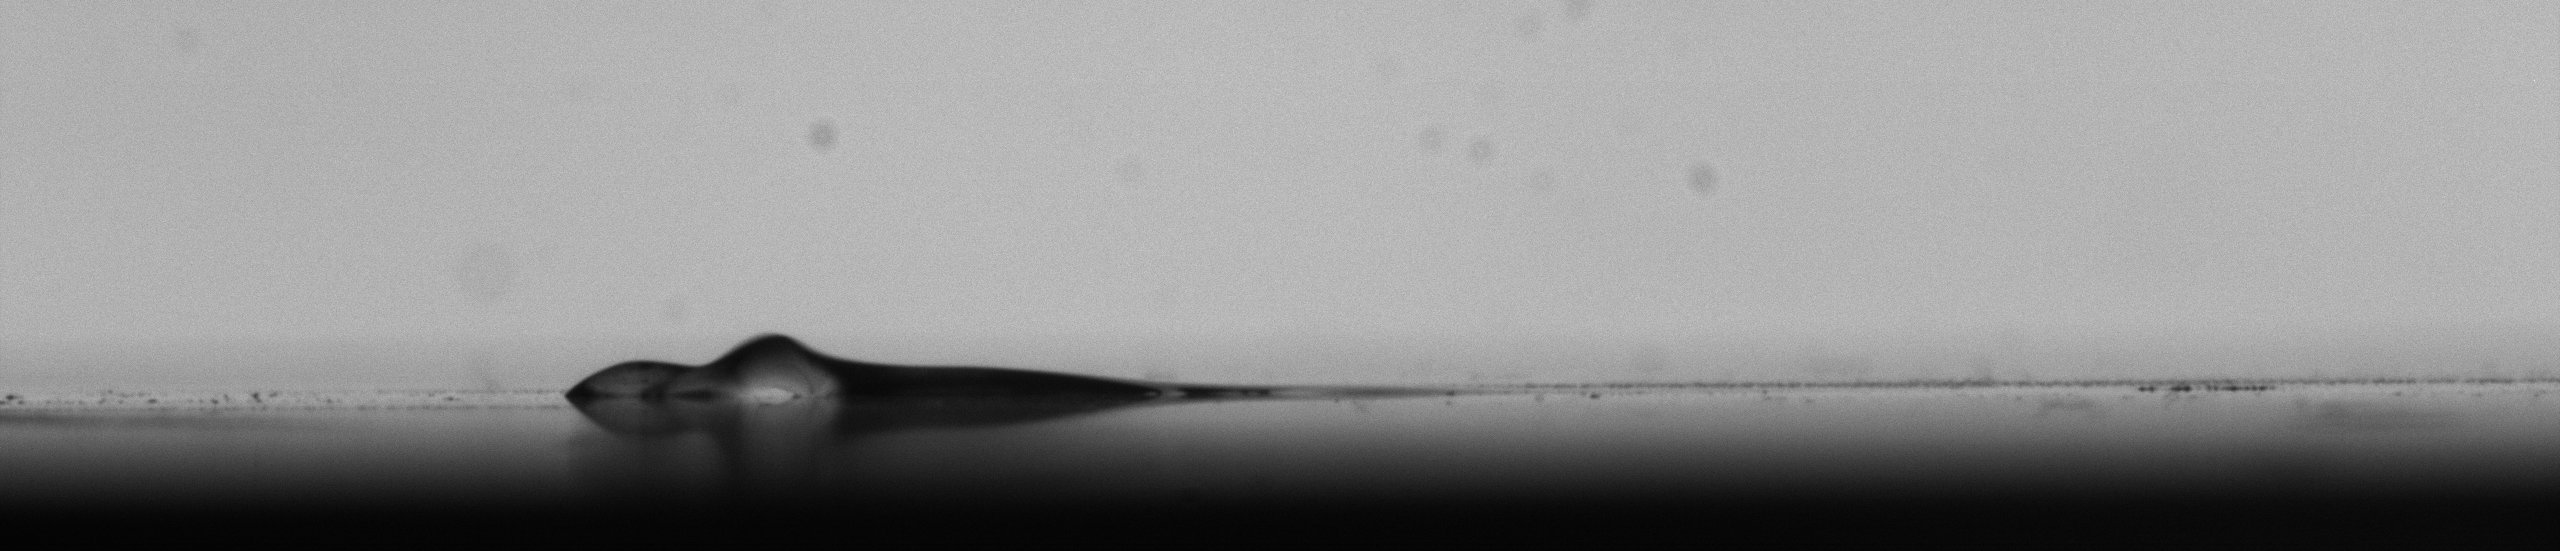
\includegraphics[height=0.2\linewidth]{gfx/test628} \\ \bigskip
        \fromUniversity\\
        \mySupervisor \\ \medskip
        \fromLab\\
        \myProf\\
        \myOtherProf \\
        \AnotherProf \\ \bigskip
        \mySubtitle \\ \medskip
        %\myDegree \\
        \spacedlowsmallcaps{\myDepartment} \\
        \spacedlowsmallcaps{\myFaculty} \\ \bigskip
        %\myUni \\ \bigskip

        \myTime%\ -- \myVersion

        \vfill

    \end{center}
  \end{addmargin}
\end{titlepage}

\thispagestyle{empty}

\hfill

\vfill

\noindent\myName: \textit{\myTitle,} \mySubtitle, %\myDegree,
\textcopyright\ \myTime

%\bigskip
%
%\noindent\spacedlowsmallcaps{Supervisors}: \\
%\myProf \\
%\myOtherProf \\
%\mySupervisor
%
%\medskip
%
%\noindent\spacedlowsmallcaps{Location}: \\
%\myLocation
%
%\medskip
%
%\noindent\spacedlowsmallcaps{Time Frame}: \\
%\myTime

%\cleardoublepage%*******************************************************
% Dedication
%*******************************************************
\thispagestyle{empty}
\phantomsection
\pdfbookmark[1]{Dedication}{Dedication}

\vspace*{3cm}

\begin{center}
    \emph{Ohana} means family. \\
    Family means nobody gets left behind, or forgotten. \\ \medskip
    --- Lilo \& Stitch
\end{center}

\medskip

\begin{center}
    Dedicated to the loving memory of Rudolf Miede. \\ \smallskip
    1939\,--\,2005
\end{center}

%\cleardoublepage\include{FrontBackmatter/Foreword}
\cleardoublepage%*******************************************************
% Abstract
%*******************************************************
%\renewcommand{\abstractname}{Abstract}
\pdfbookmark[1]{Abstract}{Abstract}
% \addcontentsline{toc}{chapter}{\tocEntry{Abstract}}
\begingroup
\let\clearpage\relax
\let\cleardoublepage\relax
\let\cleardoublepage\relax

\chapter*{Abstract}
We are studying a drop of water sliding on a horizontal plane.

\vfill


\chapter*{Résumé}
Nous faisons l'étude d'une goutte d'eau glissant sur une surface horizontale.

\endgroup

\vfill

%\cleardoublepage%*******************************************************
% Publications
%*******************************************************
\pdfbookmark[1]{Publications}{publications}
\chapter*{Publications}\graffito{This is just an early --~and currently ugly~-- test!}
This might come in handy for PhD theses: some ideas and figures have appeared previously in the following publications:

%\noindent Put your publications from the thesis here. The packages \texttt{multibib} or \texttt{bibtopic} etc. can be used to handle multiple different bibliographies in your document.

\begin{refsection}[ownpubs]
    \small
    \nocite{*} % is local to to the enclosing refsection
    \printbibliography[heading=none]
\end{refsection}

\emph{Attention}: This requires a separate run of \texttt{bibtex} for your \texttt{refsection}, \eg, \texttt{ClassicThesis1-blx} for this file. You might also use \texttt{biber} as the backend for \texttt{biblatex}. See also \url{http://tex.stackexchange.com/questions/128196/problem-with-refsection}.

%\cleardoublepage%*******************************************************
% Acknowledgments
%*******************************************************
\pdfbookmark[1]{Acknowledgments}{acknowledgments}

\begin{flushright}{\slshape
    We have seen that computer programming is an art, \\
    because it applies accumulated knowledge to the world, \\
    because it requires skill and ingenuity, and especially \\
    because it produces objects of beauty.} \\ \medskip
    --- \defcitealias{knuth:1974}{Donald E. Knuth}\citetalias{knuth:1974} \citep{knuth:1974}
\end{flushright}



\bigskip

\begingroup
\let\clearpage\relax
\let\cleardoublepage\relax
\let\cleardoublepage\relax
\chapter*{Acknowledgments}
Put your acknowledgments here.

Many thanks to everybody who already sent me a postcard!

Regarding the typography and other help, many thanks go to Marco
Kuhlmann, Philipp Lehman, Lothar Schlesier, Jim Young, Lorenzo
Pantieri and Enrico Gregorio\footnote{Members of GuIT (Gruppo
Italiano Utilizzatori di \TeX\ e \LaTeX )}, J\"org Sommer,
Joachim K\"ostler, Daniel Gottschlag, Denis Aydin, Paride
Legovini, Steffen Prochnow, Nicolas Repp, Hinrich Harms,
Roland Winkler, Jörg Weber, Henri Menke, Claus Lahiri,
Clemens Niederberger, Stefano Bragaglia, Jörn Hees,
Scott Lowe, Dave Howcroft, Jos\'e M. Alcaide, David Carlisle,
Ulrike Fischer, Hugues de Lassus, Csaba Hajdu, Dave Howcroft, 
and the whole \LaTeX-community for support, ideas and
some great software.

\bigskip

\noindent\emph{Regarding \mLyX}: The \mLyX\ port was intially done by
\emph{Nicholas Mariette} in March 2009 and continued by
\emph{Ivo Pletikosi\'c} in 2011. Thank you very much for your
work and for the contributions to the original style.


\endgroup

\cleardoublepage%*******************************************************
% Table of Contents
%*******************************************************
\pagestyle{scrheadings}
%\phantomsection
\pdfbookmark[1]{\contentsname}{tableofcontents}
\setcounter{tocdepth}{2} % <-- 2 includes up to subsections in the ToC
\setcounter{secnumdepth}{3} % <-- 3 numbers up to subsubsections
\manualmark
\markboth{\spacedlowsmallcaps{\contentsname}}{\spacedlowsmallcaps{\contentsname}}
\tableofcontents
\automark[section]{chapter}
\renewcommand{\chaptermark}[1]{\markboth{\spacedlowsmallcaps{#1}}{\spacedlowsmallcaps{#1}}}
\renewcommand{\sectionmark}[1]{\markright{\textsc{\thesection}\enspace\spacedlowsmallcaps{#1}}}
%*******************************************************
% List of Figures and of the Tables
%*******************************************************
\clearpage
% \pagestyle{empty} % Uncomment this line if your lists should not have any headlines with section name and page number
\begingroup
    \let\clearpage\relax
    \let\cleardoublepage\relax
    %*******************************************************
    % List of Figures
    %*******************************************************
    %\phantomsection
    %\addcontentsline{toc}{chapter}{\listfigurename}
    \pdfbookmark[1]{\listfigurename}{lof}
    \listoffigures

    \vspace{8ex}

    %*******************************************************
    % List of Tables
    %*******************************************************
    %\phantomsection
    %\addcontentsline{toc}{chapter}{\listtablename}
    \pdfbookmark[1]{\listtablename}{lot}
    \listoftables

    \vspace{8ex}
    % \newpage

    %*******************************************************
    % List of Listings
    %*******************************************************
    %\phantomsection
    %\addcontentsline{toc}{chapter}{\lstlistlistingname}
    \pdfbookmark[1]{\lstlistlistingname}{lol}
    \lstlistoflistings

    \vspace{8ex}

    %*******************************************************
    % Acronyms
    %*******************************************************
    %\phantomsection
    \pdfbookmark[1]{Acronyms}{acronyms}
    \markboth{\spacedlowsmallcaps{Acronyms}}{\spacedlowsmallcaps{Acronyms}}
    \chapter*{Acronyms}
    \begin{acronym}[UMLX]
        \acro{DRY}{Don't Repeat Yourself}
        \acro{API}{Application Programming Interface}
        \acro{UML}{Unified Modeling Language}
    \end{acronym}

\endgroup

%********************************************************************
% Mainmatter
%*******************************************************
\cleardoublepage
\pagestyle{scrheadings}
\pagenumbering{arabic}
%\setcounter{page}{90}
% use \cleardoublepage here to avoid problems with pdfbookmark
\cleardoublepage

%************************************************
\chapter{Introduction}\label{ch:introduction}
%************************************************

Dans le domaine des transports, avoir des gouttes de pluie sur le pare brise d'une voiture est courant et ces gouttes peuvent ruisseler sous l'action du vent.
Dans le cas de l'aéronautique, les gouttes d'eau qui ne ruissellent pas, qui ne glissent pas, peuvent givrer (devenir de petits morceaux de glace) et nuire au bon fonctionnement de l'appareil.\\

L'objectif de notre stage est d'étudier le glissement d'une goutte d'eau sur une plaque plane et d'établir le lien entre les paramètres qui régissent ce phénomène de glissement comme la taille ou les angles de contact.\\

Pour atteindre notre objectif, nous prendrons des images (à l'aide d'une caméra) de gouttes d'eau glissant sur une plaque plane dans une soufflerie et nous traiterons ensuite ces images à l'aide de Matlab pour obtenir des paramètres d'une goutte d'eau pendant son glissement, puis nous chercherons à interpréter ces données.
\cleardoublepage
%************************************************
\chapter{Couche limite}\label{ch:couche}
%************************************************

\begin{figure}[ht]
	\centering
	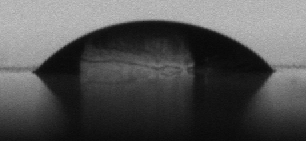
\includegraphics[scale = 0.6]{./gfx/crop_vitesse=28_volume=003.png}
	\caption{Goutte d'eau de volume $0.03$ml}
\end{figure}
Notre goutte d'eau (de volume de l'ordre millilitre) est sur une paroi horizontale en présence d'un écoulement d'air.


Pour déterminer les vitesses de l'écoulement d'air au voisinage de notre goutte d'eau, nous devons nous intéresser à la couche limite parce que d'après la théorie sur la couche limite, l'écoulement d'un fluide en présence d'une paroi peut être séparé en deux régions dont l'une proche de la paroi où les effets visqueux ne peuvent être négligés par rapport aux effets inertiels et l'autre région à l'extérieur de la précédente (avec une frontière commune) où les effets visqueux peuvent être négligés.

La couche limite est cette région proche de la paroi où les effets visqueux ne peuvent être négligés.

C'est Prandtl qui fut le premier à définir la couche limite. 

\subsection{Équations de la couche limite }

Les équations de la couche limite sont définies pour un écoulement bidimensionnel et nous nous les donnerons uniquement pour le cas d'un écoulement laminaire puisque nos écoulements étaient laminaires dans nos expériences.

Soit $u$ la vitesse de l'écoulement parallèle à la paroi suivant l'axe $x$ et $v$ la vitesse normale à la paroi suivant l'axe $y$.

Soit $U$ et $V$ les vitesses caractéristiques dans la couche limite respectivement de $u$ et $v$ ($\left| u \right| \sim U$ et $\left| v \right| \sim U$).

Soit $L$ et $\delta$ la taille caractéristique de la couche limite suivant respectivement l'axe $x$ et l'axe $y$ ($\left| x \right| \sim L$ et $\left| y \right| \sim \delta$).

En plus de l'hypothèse d'écoulement bidimensionnel, les hypothèses faites sont : la pesanteur est négligée, l'écoulement est stationnaire, incompressible, $\frac{\delta}{L} << 1$ et les effets visqueux et inertiels sont du même ordre de grandeur dans la couche limite.


De l'équation de Navier-Stokes et de continuité, on trouve pour équations de la couche limite:

\begin{align}	
	\frac{\partial u}{\partial x} 
	+
	\frac{\partial v}{\partial y} 
	&= 0 \\
	u\frac{\partial u}{\partial x} + 
	v\frac{\partial u}{\partial y} 
	&= - \frac{1}{\rho}
	\frac{\partial p}{\partial  x} +
	\nu
	\frac{\partial^{2} u}{\partial  y^{2}} \\
	\frac{\partial p}{\partial y} 
	&= 0
\end{align}
\subsection{Équations de Blasius}
L'équation de Blasius est l'équation de la couche limite pour un écoulement laminaire sur une plaque plane dont la vitesse $U$ loin de la couche limite est constante et parallèle à l'axe $x$.

Soit $\varphi$ la fonction de courant tel que :

\begin{align*}
	u(x,y) &= 
	\frac{\partial \varphi}{\partial y} \\
	v(x,y) &= - 
	\frac{\partial \varphi}{\partial x}
\end{align*}

On pose :

\begin{align*}
	\eta &= y \sqrt{\frac{U}{2\nu x }} \\
	\varphi &= \sqrt{2\nu U x} f(\eta)
\end{align*}


On trouve ainsi l'équation de la couche limite de Blasius à partir des équations de la couche limite :
\begin{equation}	
	\frac{d^{3}f}{d\eta^{3}} + f\frac{d^{2} f}{d\eta^{2}} = 0
\end{equation}
Avec les conditions aux limites:
\begin{align}
	u(x,0) &= 0 &\Rightarrow &&
	\left.
	\frac{d f}{d \eta}     \right|_{\eta = 0} &= 0
	\\
	v(x,0) &= 0 &\Rightarrow &&
	f(0) &= 0
	\\
	u(x,\infty) &= U &\Rightarrow &&
	\left.
	\frac{d f}{d \eta} \right|_{\eta = \infty} &= 1
\end{align}
\newpage
\begin{figure}[ht]
	\centering
	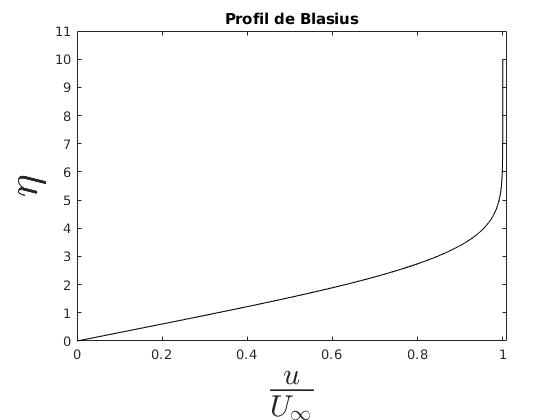
\includegraphics[scale = 0.6]{./gfx/Blasius.png}
	\caption{Profil de Blasius}
\end{figure}
Les grandeurs que nous avons comparées expérimentalement provenant du résultat des équations de Blasius sont l'épaisseur de déplacement $\delta_{1}$, l'épaisseur de quantité de mouvement $\delta_{2}$ et le coefficient de frottement $C_{f}$
\subsection{Épaisseur de déplacement}
L'épaisseur de déplacement $\delta_{1}$ à $x$ fixé est définie par:
\begin{equation}
	\delta_{1} = 
	\int_{0}^{^\infty}
	\left(
	1 - 
	\frac{u}{U}
	\right)
	dy
	\approx \frac{1.72x}{\sqrt{Re_{x}}}
\end{equation}
\subsection{Épaisseur de quantité de mouvement}
L'épaisseur de quantité de mouvement $\delta_{2}$ à $x$ fixé est définie par:
\begin{equation}
	\delta_{2} = 
	\int_{0}^{^\infty}
	\frac{u}{U}
	\left(
	1 - 
	\frac{u}{U}
	\right)
	dy
	\approx \frac{0.664x}{\sqrt{Re_{x}}}
\end{equation}
\subsection{Coefficient de frottement à la paroi}
Le coefficient de frottement à la paroi $C_{f}$ à $x$ fixé est défini par:
\begin{equation}
	C_{f} =
	\frac{2\tau_{y=0}}{\rho U^{2}} =
	\frac{2\nu}{U^{2}}
	\left.
	\frac{\partial u}{\partial y}
	\right|_{y = 0} \approx \frac{0.664}{\sqrt{Re_{x}}}
\end{equation}
\subsection{Comparaisons avec nos expériences}
Nous avons effectué nos mesures à l'aide de l'anémomètre à fil chaud et nous trouvons avec :
\begin{align*}
	x &= 0.55m\\
	Re_{x} &= \frac{Ux}{\nu}\\
	\nu &= 1.5e-5 m^{2}.s^{-1}~~\text{à}~~T = 25^{o}C; 
\end{align*}
\begin{table}[ht]
	\centering
	\begin{tabular}{cc}
		\hline\\
		$U(m/s)$ & Reynolds\\
		\hline
   15 & 550000.00\\
   20 & 733333.33\\
   24 & 880000.00\\
   28 & 1026666.7
	\end{tabular}
	\caption{Nombre de Reynolds $Re_{x}$}
\end{table}
\begin{table}[ht]
	\centering
	\begin{tabular}{cccc}
		\hline\\
		$U(m/s)$ & $\delta_{1Blasius}(mm)$ &
		$ \delta_{1Experience}(mm)$ & 
		 erreur relative\\
		\hline
		15   & 1.27   & 1.24   & 2.69\%\\
		20   & 1.11   & 1.10   & 0.61\%\\
		24   & 1.02   & 0.99   & 3.13\%\\
		28   & 0.96   & 0.95   & 1.55\%
	\end{tabular}
	\caption{Comparaison épaisseur de déplacement $\delta_{1}$}
\end{table}
\begin{table}[ht]
	\centering
	\begin{tabular}{cccc}
		\hline\\
		$U(m/s)$ & $\delta_{2Blasius}(mm)$ &
		$ \delta_{2Experience}(mm)$ & 
		 erreur relative\\
		\hline
   15 & 0.49   & 0.47   & 3.64\%\\
   20 & 0.43   & 0.41   & 4.62\%\\
   24 & 0.40   & 0.37   & 6.08\%\\
   28 & 0.37   & 0.35   & 6.92\%
	\end{tabular}
	\caption{Comparaison épaisseur de quantité de mouvement $\delta_{2}$}
\end{table}
\begin{table}[ht]
	\centering
	\begin{tabular}{cccc}
		\hline\\
		$U(m/s)$ & $C_{fBlasius}$ &
		$ C_{fExperience}$ & 
		 erreur relative\\
		\hline
   15 & 8.92e-04   & 9.19e-04   & 2.89\%\\
   20 & 7.77e-04   & 7.67e-04   & 1.31\%\\
   24 & 7.20e-04   & 7.33e-04   & 1.85\%\\
   28 & 6.75e-04   & 6.67e-04   & 1.26\%
	\end{tabular}
	\caption{Comparaison coefficient de frottement $C_{f}$}
\end{table}
\begin{figure}[ht]
	\centering
	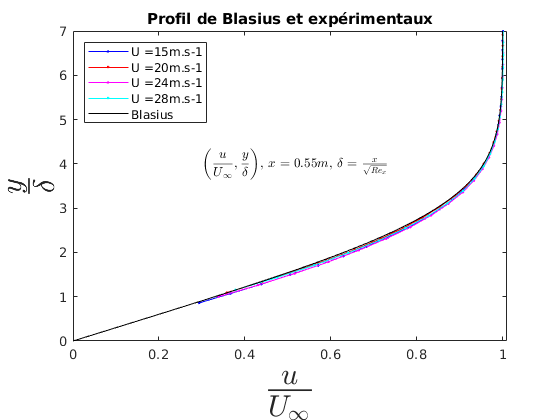
\includegraphics[scale = 0.6]{./gfx/Bla.png}
	\caption{Profil de Blasius et expérimentaux}
\end{figure}
\newpage
Nous avons pu constater que l'épaisseur de la couche limite, l'épaisseur de la quantité de mouvement, le coefficient de frottement à la paroi et nos profils de vitesses sont tous très proches de leur équivalent dans la théorie de la couche limite de Blasius.
%\begin{thebibliography}{}
%\bibitem{RefJ}
%% Format for Journal Reference
%Author, Article title, Journal, Volume, page numbers (year)
%% Format for books
%\bibitem{RefB}
%Author, Book title, page numbers. Publisher, place (year)
%\end{thebibliography}

%\addtocontents{toc}{\protect\clearpage} % <--- just debug stuff, ignore
%************************************************
\chapter{Capillarité}\label{ch:capillaire}
%************************************************

\section{Tension de surface}
\begin{figure}[ht]
	\centering
	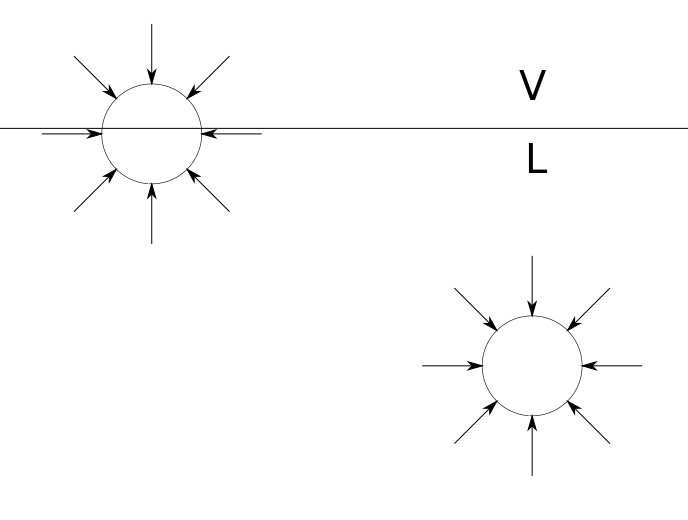
\includegraphics[scale = 0.3]{./gfx/rondforces.png}
	\caption{Molécule de liquide}
\end{figure}

La tension de surface est une force par unité de longueur.\\ 

Dans un liquide ayant une interface, une molécule complètement immergée dans le liquide est soumise à des forces d'interactions avec les autres molécules (du liquide) dans toutes les directions. 

Une molécule située à l'interface, la somme des interactions (avec les molécules du même fluide) est non nulle est dirigée vers l'intérieur du liquide. Il existe donc une force supplémentaire qui permet de maintenir l'interface.

Cette force supplémentaire (par unité de longueur) est la tension de surface.\\



la tension de surface est aussi une énergie par unité de surface, c'est l'énergie (par unité de surface) pour séparer les interfaces et les envoyer à l'infini l'une par rapport à l'autre.


\section{Mouillage}
Le mouillage est l'action de mouiller et mouiller consiste à  mettre en contact avec un liquide.\\


C'est le paramètre d'étalement $S = \gamma_{SV} - (\gamma_{SL} + \gamma_{LV}) = \gamma_{LV}(\cos\theta_{E} - 1)$ qui caractérise le mouillage lorsque la goutte est en équilibre sur un support matériel.

Quand $S > 0$, on parle de mouillage total et quand $S < 0$, on parle de mouillage partiel.\\

Nous nous intéressons en particulier à une goutte dont le support est une plaque plane dans les conditions de mouillage partiel. 
\begin{figure}[ht]
	\centering
	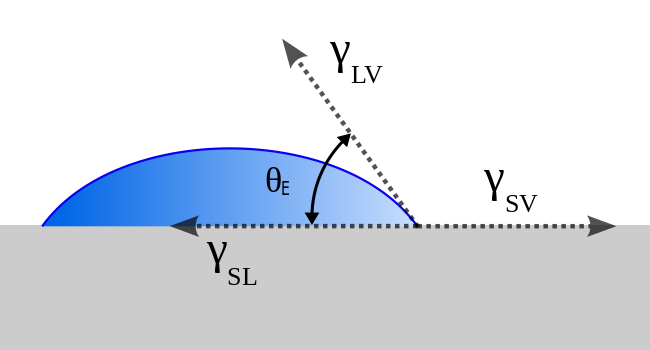
\includegraphics[scale = 0.3]{./gfx/Contact_angle2.png}
	\caption{Ligne triple}
\end{figure}



Le substrat est le nom donné au support (solide ou liquide) sur lequel la goutte de liquide repose.

Lorsqu'une goutte d'eau est posée sur support solide, il y a formation de 3 interfaces et donc de 3 tensions de surface.


En projetant les tensions de surface sur l'horizontale on obtient :

\begin{equation}
	\label{eq:Young}
	\gamma_{SV}  = \gamma_{SL} + \gamma_{LV}\cos\theta_{E}
\end{equation}

C'est la loi de Young.

\section{Hystérésis}


\begin{figure}[ht]
	\label{fig:hysteresis}
	\centering
	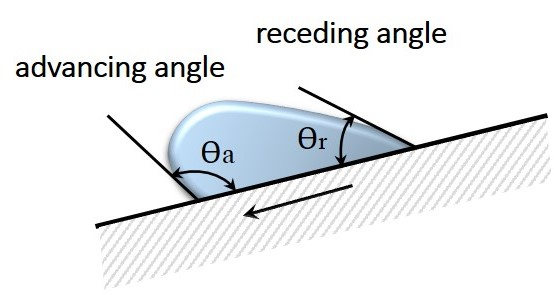
\includegraphics[scale = 0.8]{./gfx/hysteresis.jpg}
	\caption{Hystérésis}
\end{figure}
Dans la réalité l'angle statique $\theta_{E}$ n'est pas unique et on a :

\begin{equation}
	\theta_{R} <= \theta_{E} <= \theta_{A}
\end{equation}

Lorsque l'angle de contact $\theta$ vérifie $\theta < \theta_{R}$, la goutte se met à reculer et l'angle de contact $\theta$ à l'arrière de la goutte est appelé $\theta_{r}$.\\

Lorsque l'angle de contact $\theta$ vérifie $\theta > \theta_{A}$, la goutte se met à avancer et l'angle de contact $\theta$ à l'avant de la goutte est appelé $\theta_{a}$.\\

Dans le cas d'un surface parfaite $\theta_{a}$ et $\theta_{r}$ sont égaux.\\

L'hystéréris (en parlant d'angle de contact) est la différence $\theta_{a}-\theta_{r}$.

\section{Modèles d'angle dynamique}

L'angle de contact de la goutte en mouvement (l'angle dynamique) est différent de l'angle de contact quand la goutte est en équilibre (angle statique).

Seuls des modèles existent pour estimer l'angle de contact dynamique et tous ses modèles se placent dans le cas d'une surface parfaite où on ne tient pas compte de l'hystérésis. 

Ces modèles font intervenir le nombre capillaire $C_{a}$, un longueur macroscopique $b$ et une longueur miscropique $a$.
\begin{equation}
	C_{a} 
	= \frac{\text{effets visqueux}}{\text{effets capillaires}} 
	= \frac{\eta U}{\gamma}
\end{equation}
\subsection*{Modèle De Gennes} 

\begin{equation}
	\label{modele:gennes}
	\theta 
	\left(\theta^{2} - \theta_{s}^{2}\right) 
	= \pm 6\ln\left(\frac{b}{a}\right)C_{a}
\end{equation}
\subsection*{Modèle Cox et Voinov}  

\begin{equation}
	\label{modele:Cox}
	\theta^{3} - \theta_{s}^{3} = 
	\pm 
	9\ln\left(
	\frac{b}{a}\right) C_{a}
\end{equation}
\subsection*{Modèle de cinétique moléculaire}  

\begin{equation}
	\left(\theta^{2} - \theta_{s}^{2}\right) 
	\propto C_{a}
\end{equation}
\subsection*{Modèle linéaire} 

\begin{equation}
	\theta - \theta_{s} \propto \pm U
\end{equation}


%************************************************
\chapter{Expériences}\label{ch:experiences}
%************************************************
\section{Dispositif expérimental}

Nous avions à notre disposition pour effectuer nos mesures : une soufflerie, un capteur de pression pouvant aller jusqu'à $500Pa$, un capteur de température, d'une surface ayant un petit trou par où la goutte est injectée par en dessous, une seringue de capacité $5ml$, d'un injecteur qui contrôle le volume de la goutte à injecter, d'un écran laser pour bien visualiser notre goutte et d'un ordinateur pour observer les images prises par la caméra.

\begin{figure}[!hb]
\centering
	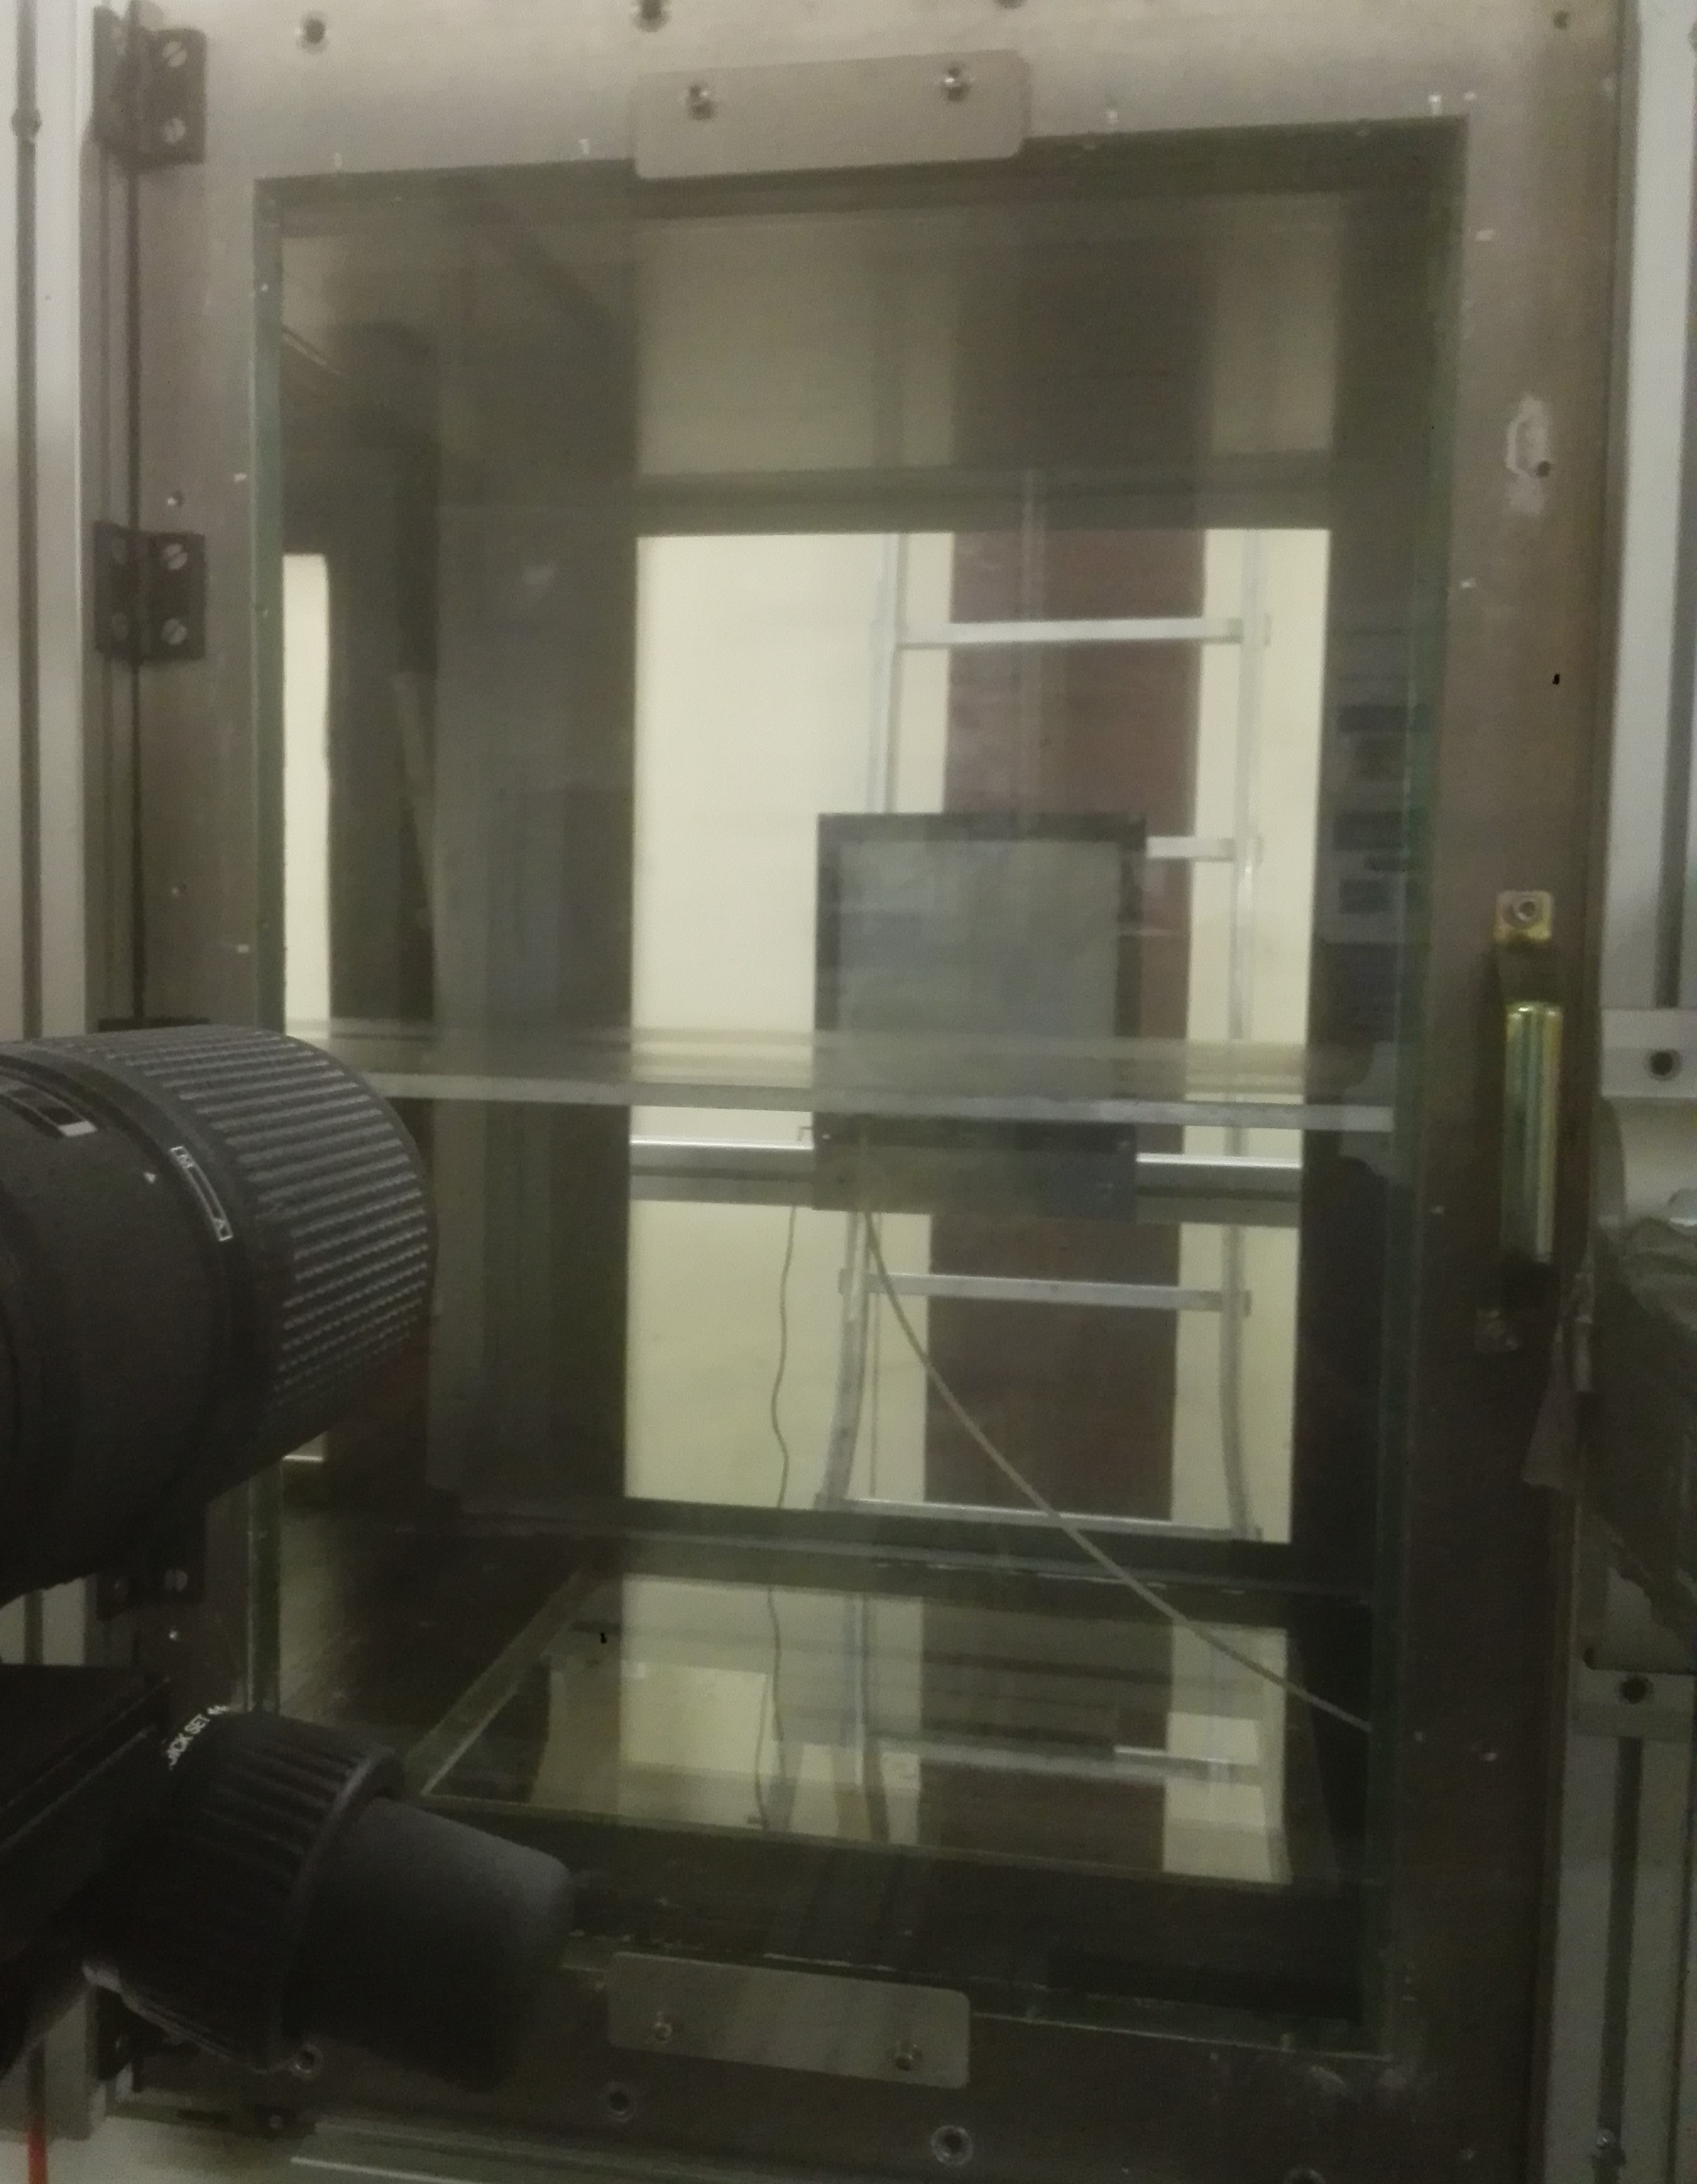
\includegraphics[width = 0.4\linewidth]{./gfx/Surface.jpg}
	\caption{Camera, surface et écran à laser}
	\label{fig:Plan}
\end{figure}
\begin{figure}[!hb]
\centering
	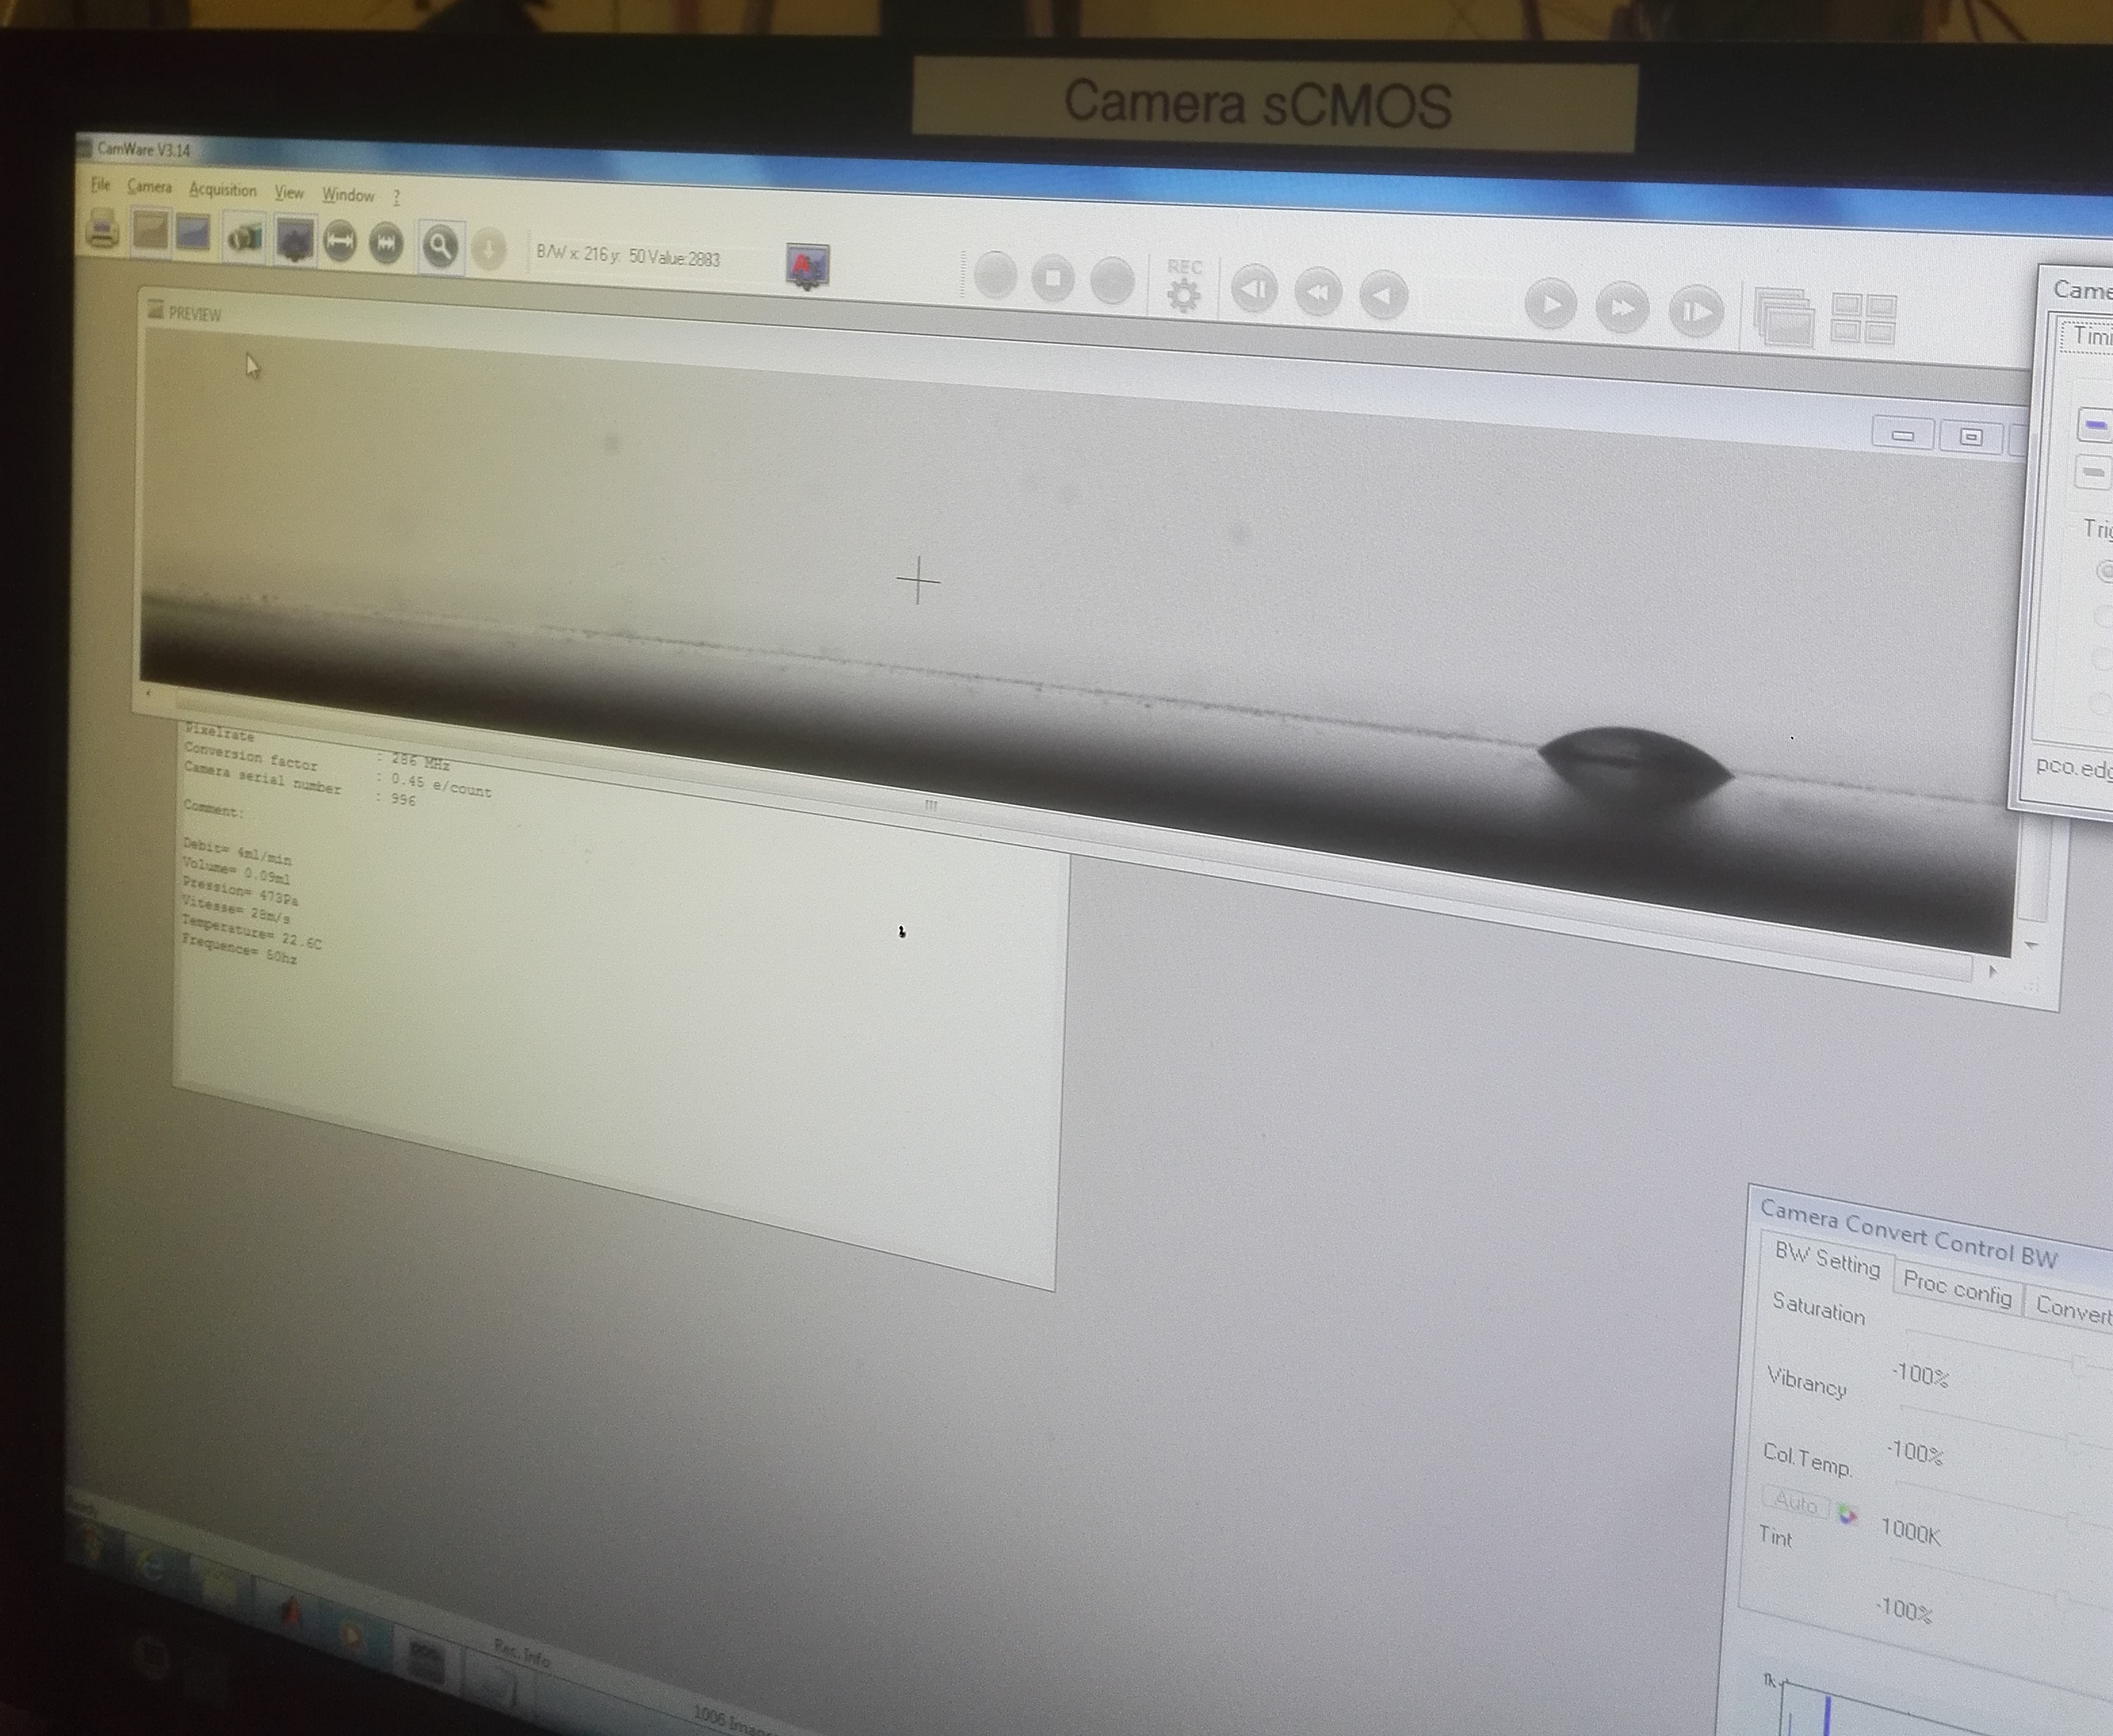
\includegraphics[width = 0.5\linewidth]{./gfx/Ecran.jpg}
	\caption{Ecran d'observation}
	\label{fig:Ecran d'observation}
\end{figure}


\section{Anémomètre à fil chaud}
C'est l'anémomètre à fil chaud qui nous a permis de déterminer les profils de la couche limite dans notre écoulement.

Le principe de l'anémomètre à fil chaud est de placer un fil chaud (de l'ordre de $1mm$ de long et de $1\mu m$ de diamètre) dans l'écoulement et de maintenir sa température constante.

l'écoulement retirera une énergie au fil chaud et pour maintenir la température constante du fil chaud, on lui fournit une certaine énergie et cette énergie fournie (la tension qu'il a fallu fournir) est liée à la vitesse au niveau du fil chaud.


\section{Paramètres mesurés}

\begin{figure}[!ht]
	\centering
	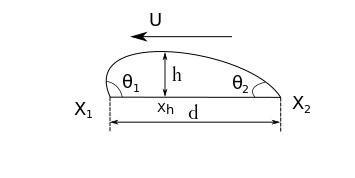
\includegraphics[scale = 1]{./gfx/rrgou2.png}
	\caption{Paramètres mesurés}
\end{figure}
\begin{figure}[!ht]
	\centering
	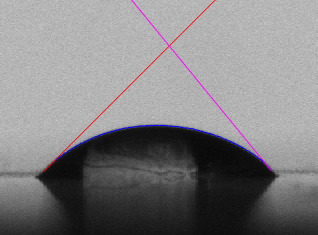
\includegraphics[scale = 0.5]{./gfx/crop_tvitesse=28_volume=003.png}
	\caption{Goutte d'eau de volume $0.03$ml avec: \\$U = 0$, $\theta_{a} = \ang{45}$, $\theta_{r} = \ang{50.17}$, $x_{1} = 14.66mm$, $x_{2} = 6.77mm$,\\ $d = 7.89mm$, $h = 4.86mm$ et $x_{h} = 48mm$}
\end{figure}


L'objectif du stage était de réussir à ressortir la courbe du contour d'une goutte à partir des photos prises avec notre caméra à la fréquence de $50Hz$ et de pouvoir extraire les paramètres comme les angles de contact, la position avant et arrière de la goutte ou la hauteur maximale de la goutte et la position où on obtient cette hauteur maximale.

\section{Mesures numériques}

Nous avons déterminé le contour de la goutte à l'aide de la fonction de Matlab \emph{bwboundaries} qui nous donnait (après avoir réussi à faire les ajustements pour cibler notre zone d'intérêt) le contour sous forme de nuage points.

Ce fut une étape assez difficile dont on a trouvé une solution qui nous satisfaisait assez tardivement (avoir le contour et la position des points extrêmes ($x_{1}$ et $x_{2}$) ont posé beaucoup de difficulté).  \\

Une fois le nuage de points définissant le contour ayant été obtenu, obtenir les tangentes aux deux extrémités de la goutte nous a aussi pris assez de temps.

Nous avons essayé de trouver des courbes d'interpolation autour de chaque extrémité (les points dont nous voulions les tangentes), mais les différentes fonctions d'interpolation de Matlab ou nos différentes méthodes n'arrivaient pas à être visuellement proche de la tangente attendue lorsque la goutte changeait de forme.\\

Nos gouttes prenaient des formes plus proche d'une courbe paramétrée en coordonnées polaires comme une cardioïde, les formes des gouttes étaient aussi souvent proche des coniques et les méthodes d'interpolation, en particulier celle se basant sur la recherche des polynômes d'ordre 2 ou plus, s'éloignaient très souvent des tangentes attendues visuellement.\\

C'est l'interpolation par un polynôme d'ordre 1 qui donnait des résultats toujours proche des tangentes qu'on pouvait s'attendre visuellement, mais le nombre de points pris pour déterminer notre tangente avec la fonction \emph{polyfit} de Matlab jouait un rôle important.

Sur un cas particulier, nous pouvions ajuster le nombre de points pour avoir une meilleure tangente (visuellement).

Notre difficulté était de faire un algorithme pour traiter des milliers d'images qui arrive à ajuster le nombre de points.

Nous partions de $n$ points (le maximum entre 2 et $1\%$ du nombre de points dans notre nuage de points) puis nous trouvions les tangentes avec $n$ et $n+1$ points.

Si les tangentes avec $n$ et $n+1$ points faisaient entre elles un angle inférieur à $\ang{0.5}$, nous conservions la tangente faite avec $n$ points, sinon on posait $n = n+1$ et on recommençait.

Si nous n'arrivions pas à avoir un angle inférieur à \ang{0.5}  entre les tangentes avec $n$ points et avec $n+1$ points, nous ne conservions pas l'image dans nos résultats faute de ne pouvoir avoir les angles de contact assez précisément.

\section{Mesures expérimentales}

Nos mesures dans la soufflerie ont été effectuées de 2 manières.\\

D'abord, nous mettions en marche la soufflerie jusqu'à ce que la vitesse se stabilise puis on injectait le volume de goutte désiré.

La difficulté de cette méthode est que la goutte d'eau se mettait souvent en mouvement avant la fin d'injection, avant d'atteindre le volume désiré.\\

Avec l'autre méthode, nous injections d'abord la goutte d'eau de volume désiré (la soufflerie à l'arrêt) et c'est par la suite que nous mettions la soufflerie en marche.

Dans ce cas, la vitesse de la soufflerie prends un temps (relativement court) à se stabiliser et nous n'avons donc pas la vitesse désirée toute suite.\\

C'est cette dernière méthode où le débit n'était pas un paramètre important que nous présenterons les résultats et nous ferons un comparatif d'un cas où le débit jouait un rôle important.
\newpage
\section{Résultat}

Nous commençons par présenter les figures \ref{fig:entre_xaxrd} et \ref{fig:entre_oaor} qui illustre bien l'ensemble de nos observations.\\

On observe la position de l'avant $x_{a}$ de la goutte se met à avancer quand la longueur $d$ augmente et lorsque cette longueur $d$ diminue, c'est la position de l'arrière $x_{r}$ qui bouge.

Cela traduit le fait que la goutte commence à bouger si l'avant ou l'arrière bougent, l'arrière pouvant commencer à bouger avant l'avant et vice-versa.\\

Pour les angles de contact, on observe que l'angle à l'avant $\theta_{a}$ commence initialement à augmenter quand la longueur $d$ de la goutte augmente, puis $\theta_{a}$ oscille avec des grandes amplitudes autour de \ang{50}.

L'angle de contact arrière $\theta_{r}$ commence lui par diminuer quand la longueur $d$ augmente puis $\theta_{r}$ se met à osciller avec de faibles amplitudes autour de $\ang{5}$.\\

Les oscillations correspondent à des mouvements oscillant de la goutte qui oscillait en reculant et en avançant rapidement autour d'une même position avant d'avancer subitement.

\newpage
\begin{figure*}[!ht]
	\centering
	\begin{minipage}{0.7\linewidth}
		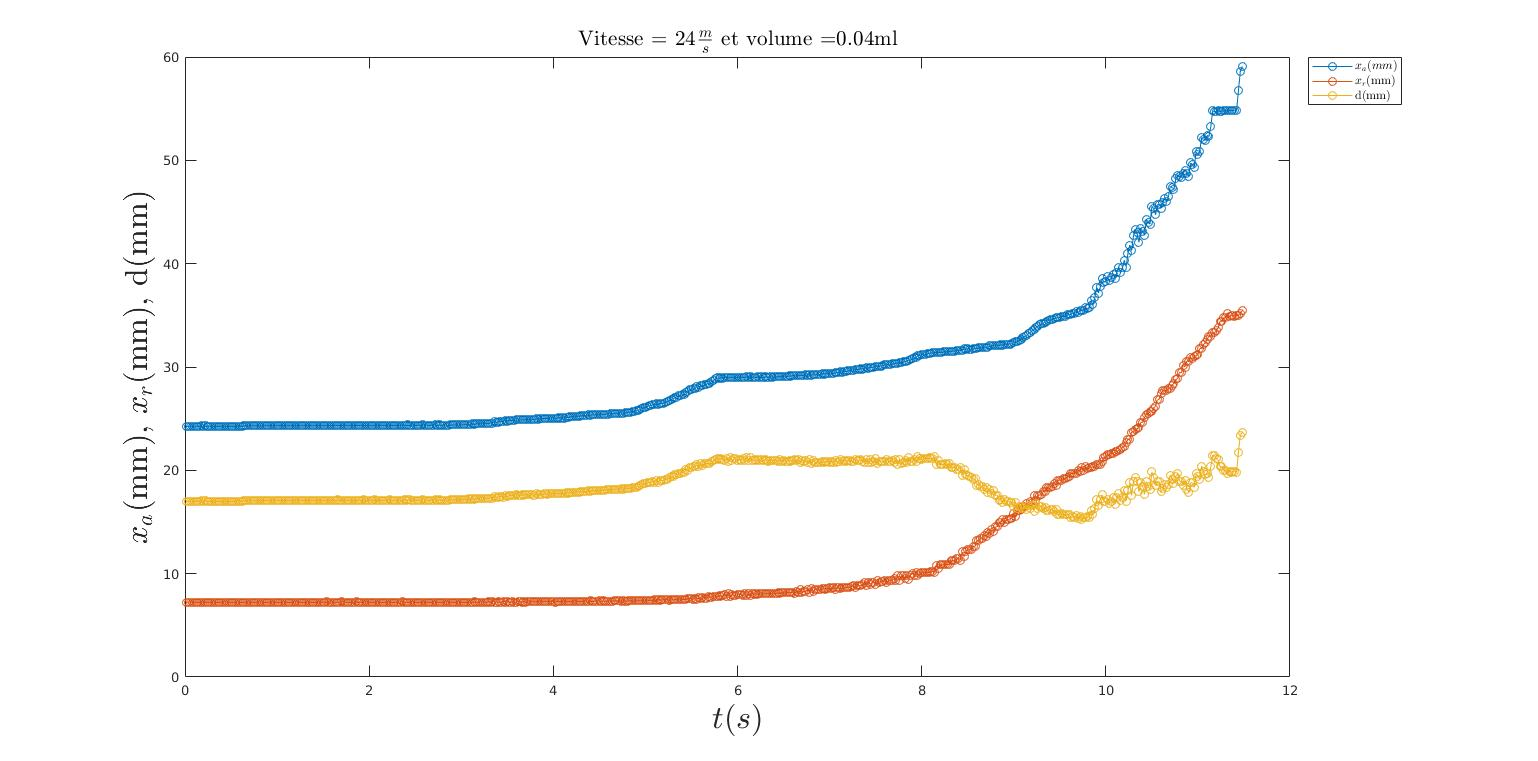
\includegraphics[width=\linewidth]{./gfx/v=24_vol=004_xaxrd.jpg}
		\caption{$\textcolor{blue}{x_{a}}$,
		$\textcolor{red}{x_{r}}$, $\textcolor{yellow}{d}$, 
		$U_{\infty}=24m.s^{-1}$, volume =$0.04ml$}
		\label{fig:entre_xaxrd}
	\end{minipage}
	\vfill
	\begin{minipage}{0.7\linewidth}
		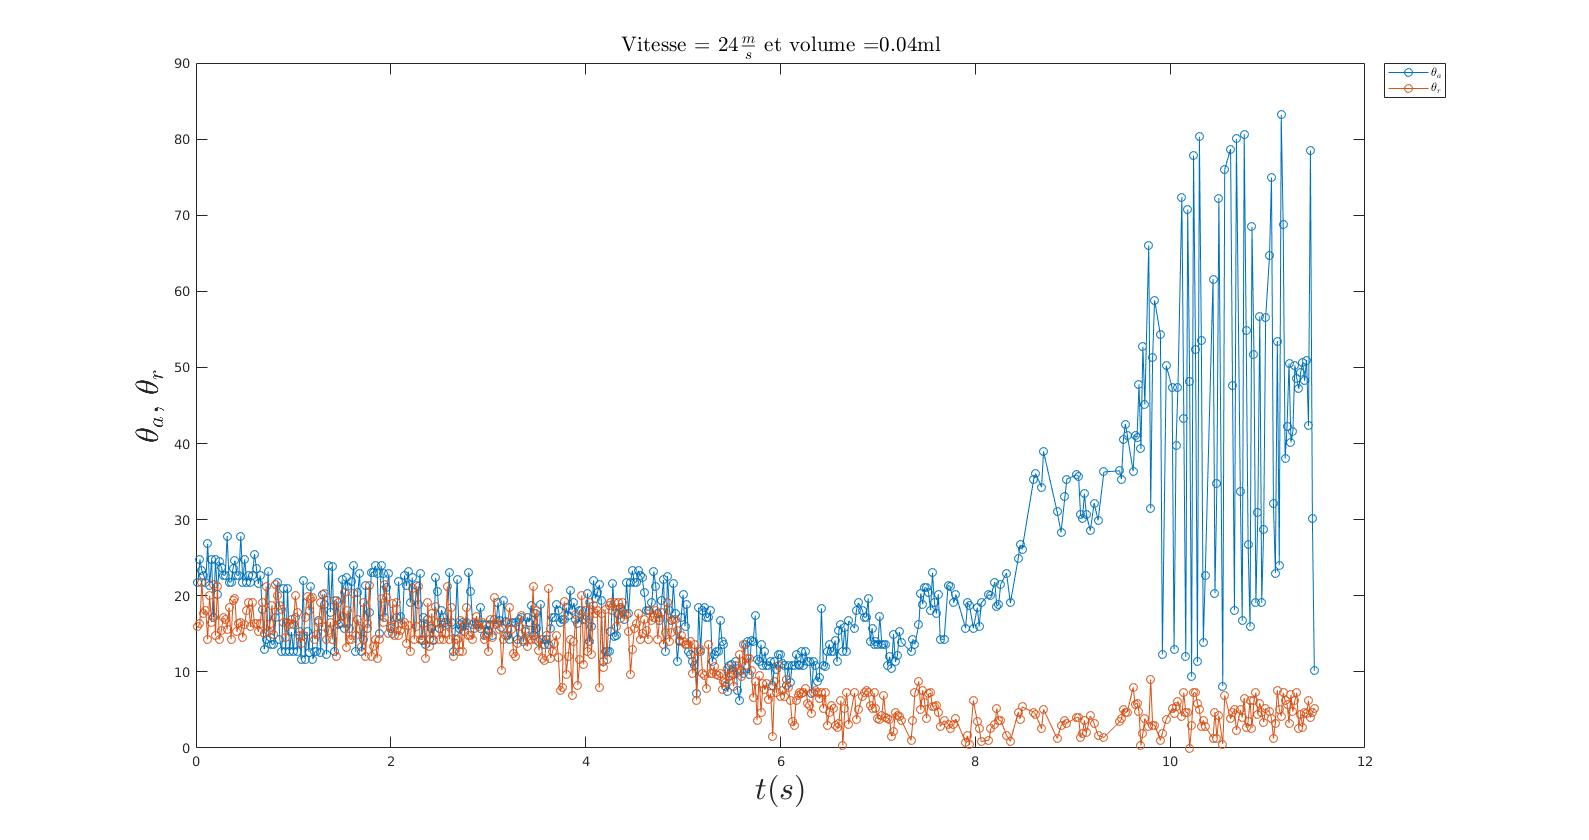
\includegraphics[width=\linewidth]{./gfx/v=24_vol=004_oaor.jpg}
		\caption{$\textcolor{blue}{\theta_{a}}$,
		$\textcolor{red}{\theta_{r}}$, $U_{\infty}=24m.s^{-1}$, volume =$0.04ml$}
		\label{fig:entre_oaor}
	\end{minipage}
 \end{figure*}


\newpage
\subsection{Vitesse de $20m.s^{-1}$}

On observe sur la figure \ref{fig:v=20d} que la longueur $d$ reste presque constante pendant un certain temps (les angles $\theta_{a}$ et $\theta_{r}$ restant eux aussi constant) et ensuite la longueur peut diminuer ou avancer.\\

On constate aussi que la longueur $d$ de la goutte commence à osciller à partir d'une certaine longueur.\\

On observe que les angles de contact évoluent de manière similaire pour toutes les gouttes : l'angle d'avancée commence à augmenter puis oscille autour de \ang{50}, l'angle de recul diminue puis oscille aux alentours de \ang{5}.\\

Les oscillations observées sont liées à la forme de la goutte et peuvent être mise en évidence avec la position et la hauteur maximale de la goutte (illustré figure \ref{fig:v=20xm} et \ref{fig:v=20ym}).\\

Nous observons que la hauteur maximale de la goutte $y_{max}$, après une phase initiale où elle est presque constante, elle peut se mettre à baisser ou à augmenter, mais lorsque $y_{max}$ augmente et atteint une certaine hauteur, $y_{max}$ se met à osciller autour de cette hauteur.
\newpage
\begin{figure}[!ht]
		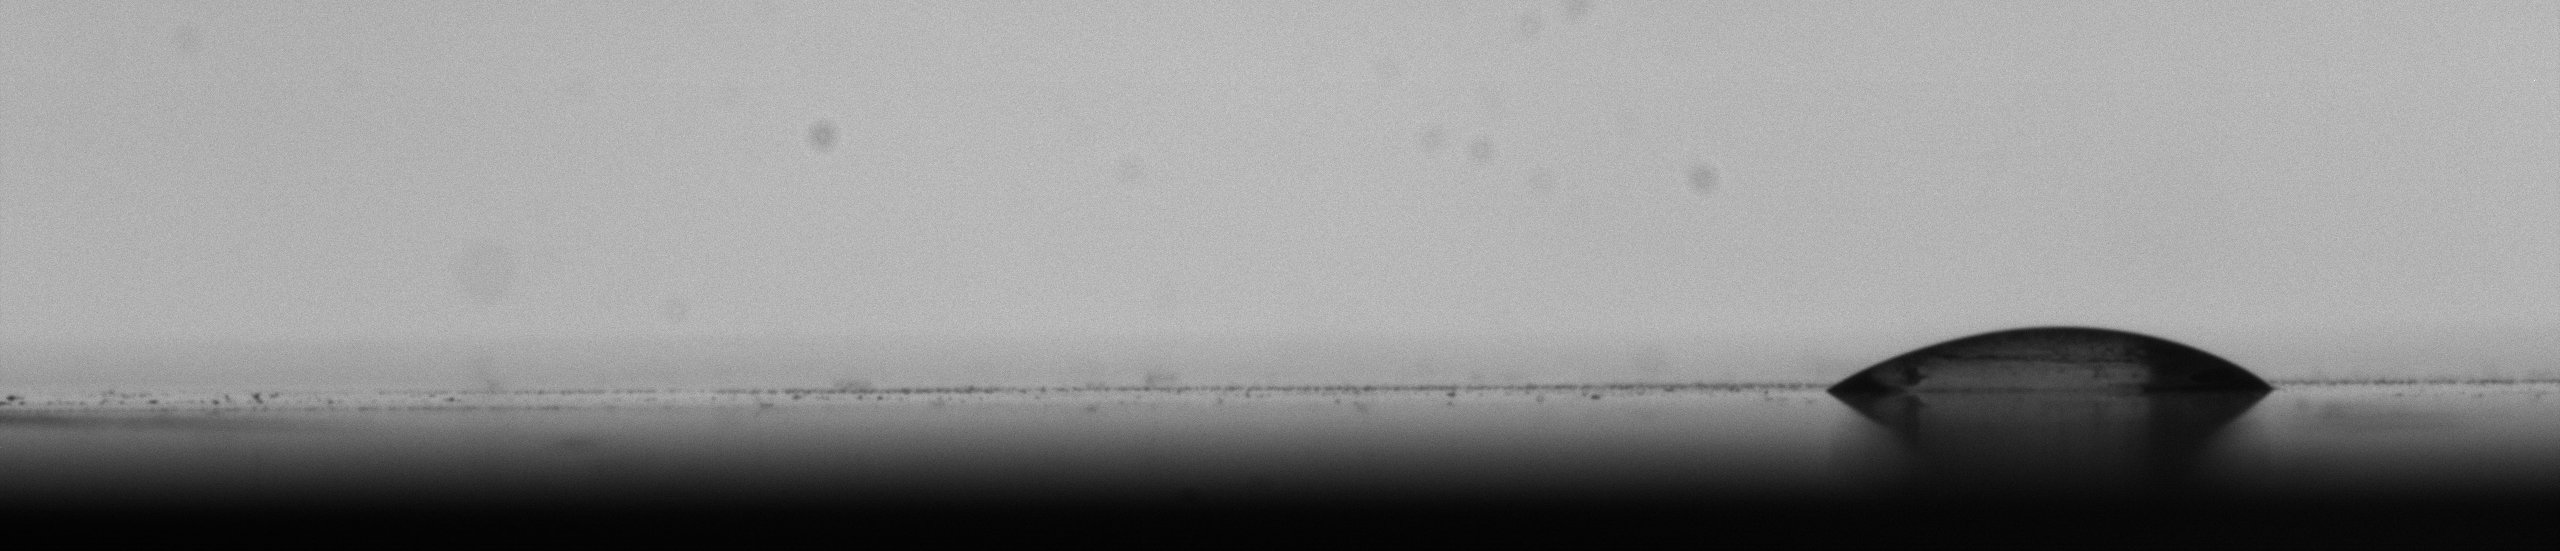
\includegraphics[width = \linewidth]{./gfx/test.jpg}
		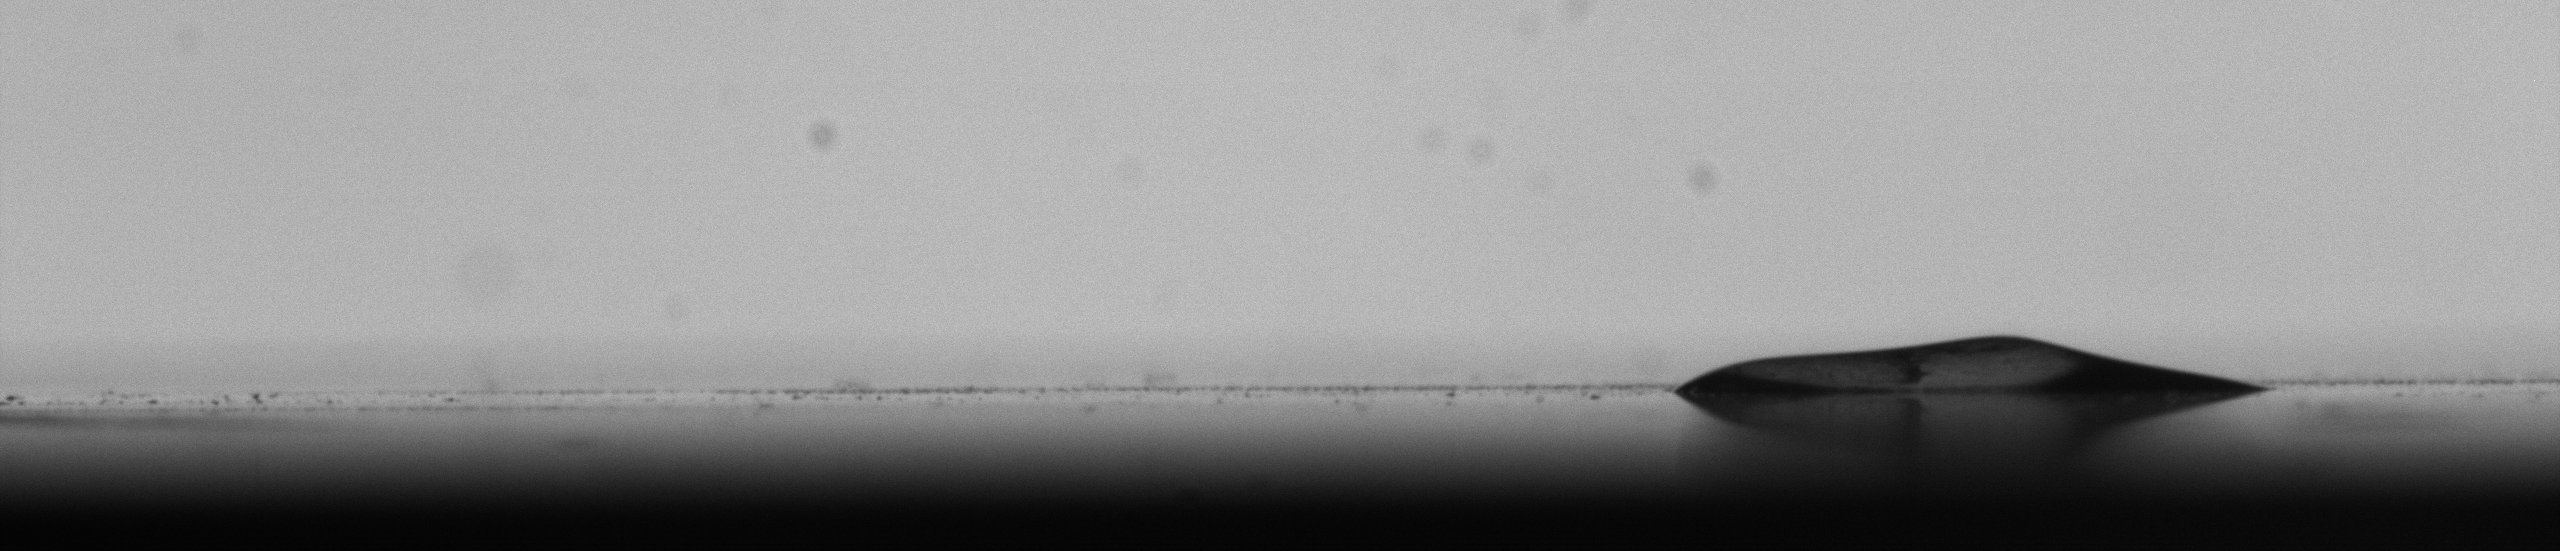
\includegraphics[width = \linewidth]{./gfx/test400.jpg}
		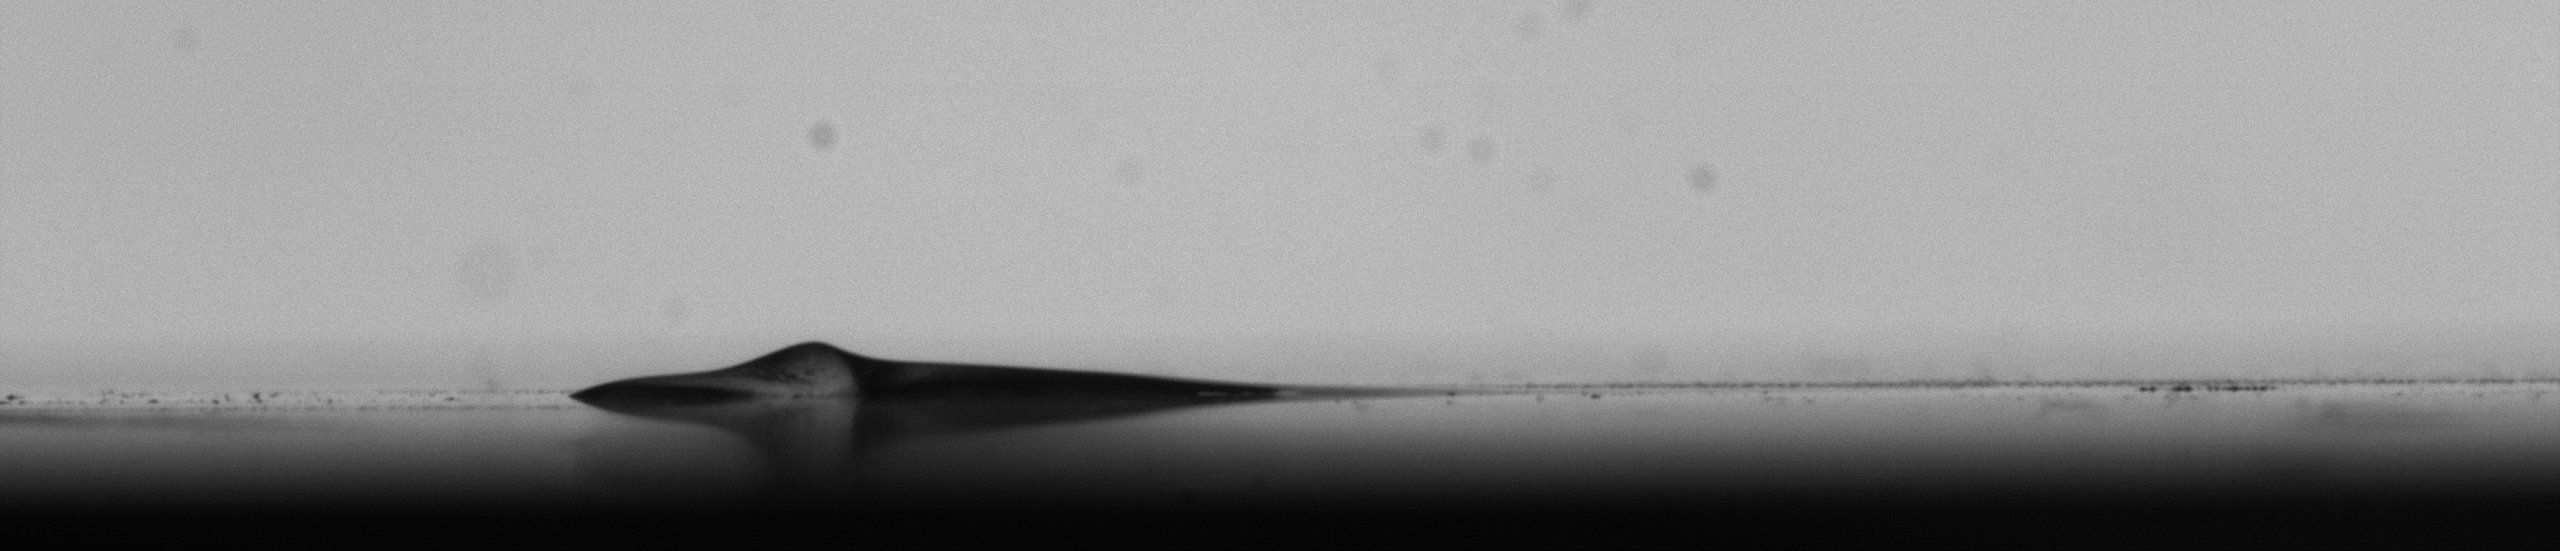
\includegraphics[width = \linewidth]{./gfx/test626.jpg}
		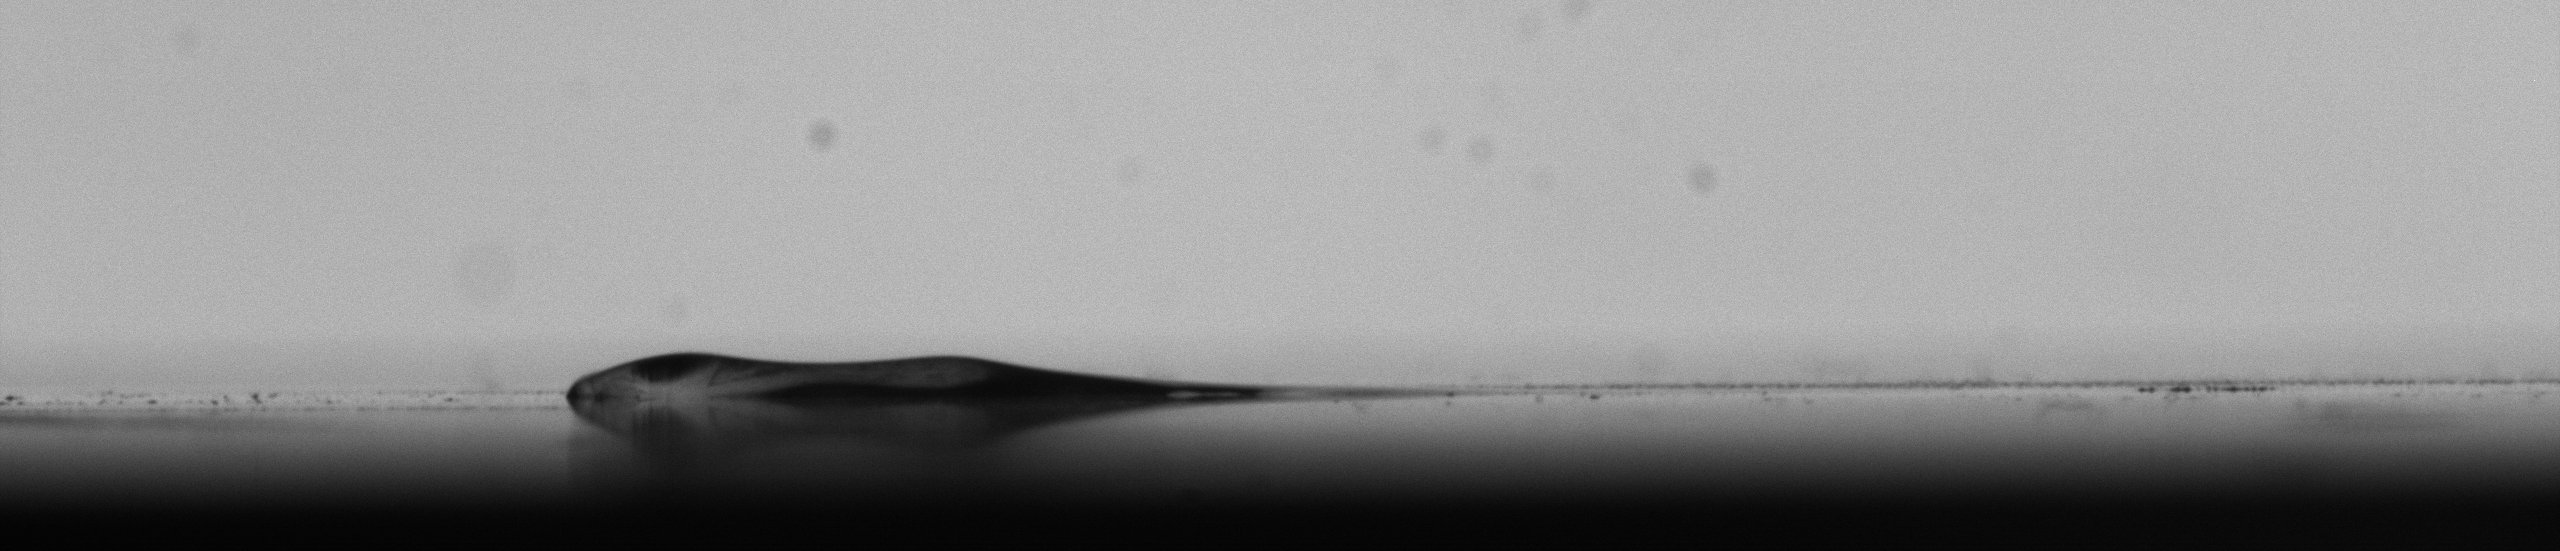
\includegraphics[width = \linewidth]{./gfx/test627.jpg}
		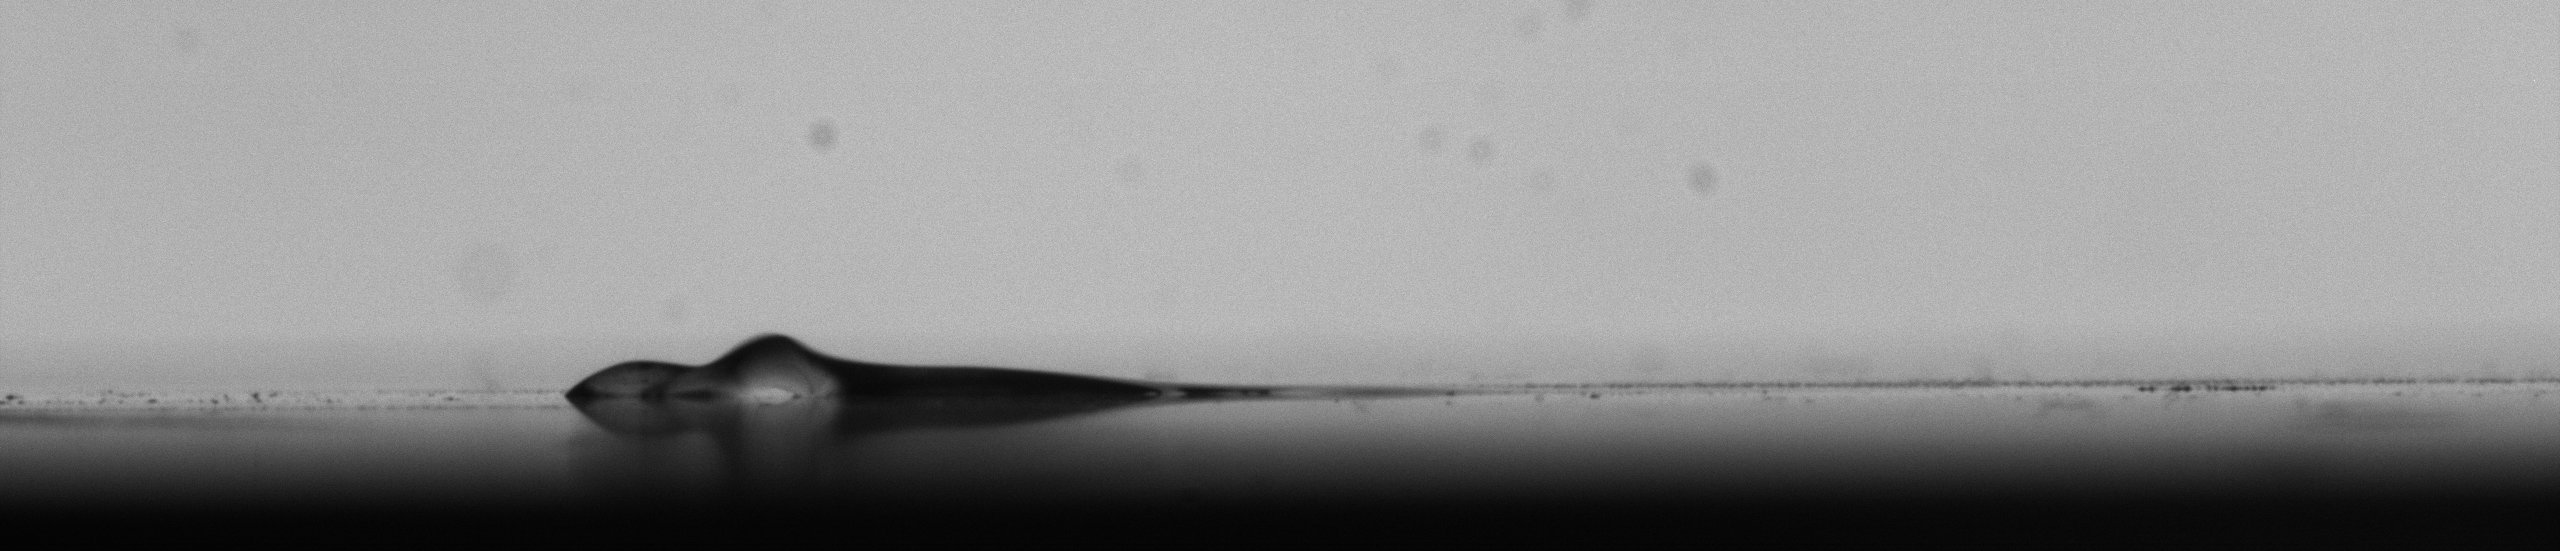
\includegraphics[width = \linewidth]{./gfx/test628.jpg}
		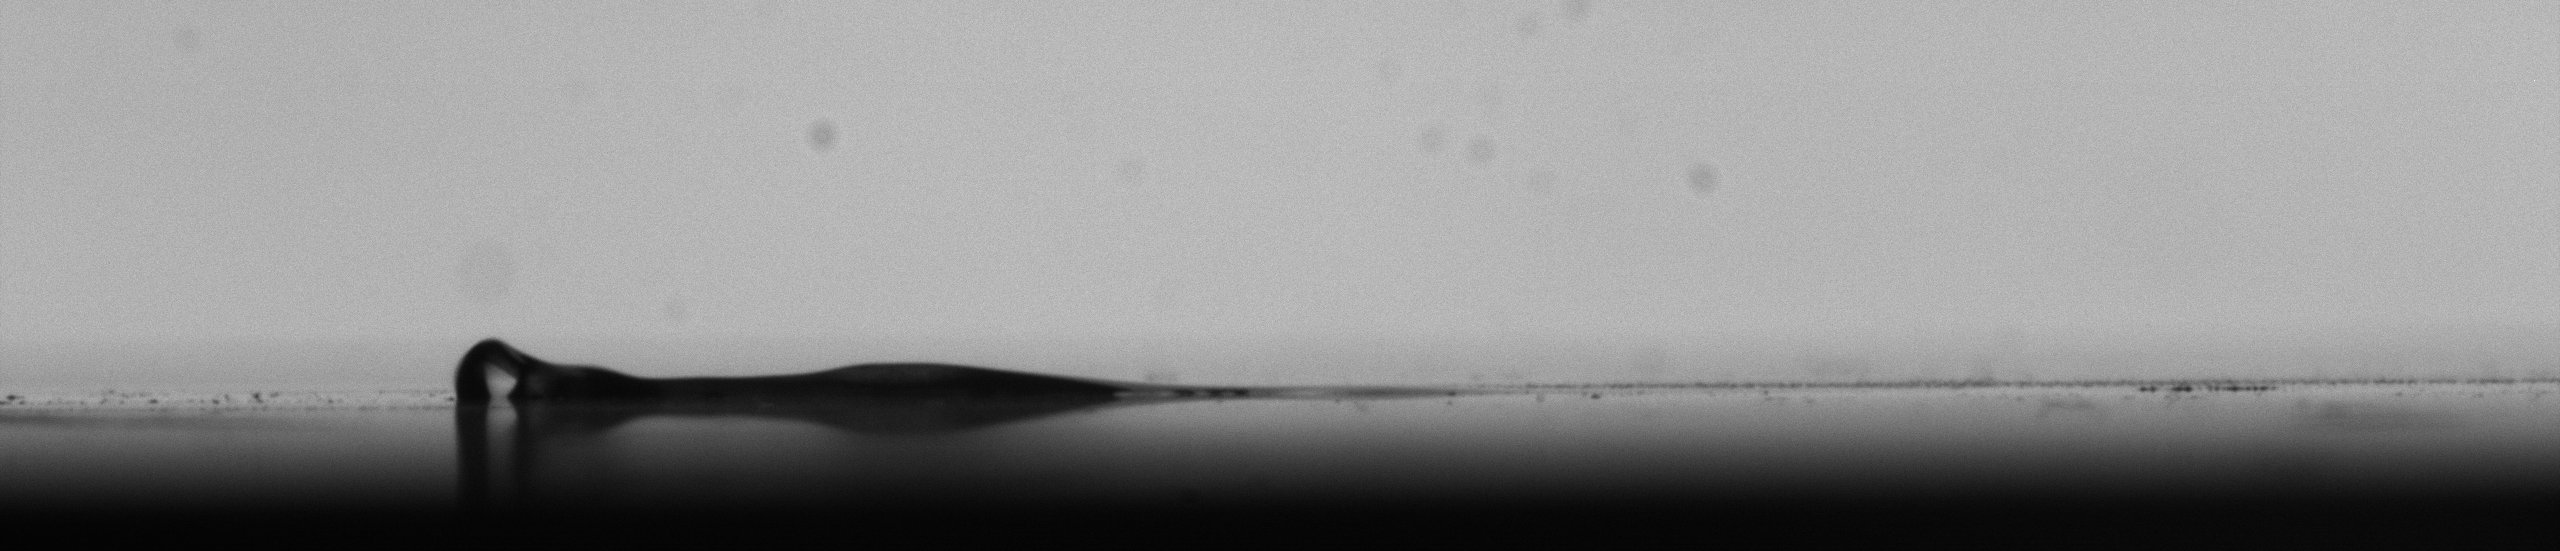
\includegraphics[width = \linewidth]{./gfx/test629.jpg}
	\caption{$U_{\infty}=20m.s^{-1}$, de haut en bas,\\	
	$t = ~0,~8,~12.52,~12.54,~12.58s$}
		\label{fig:test}
\end{figure}

\newpage

\begin{figure}[!ht]
	\begin{minipage}{0.7\linewidth}
		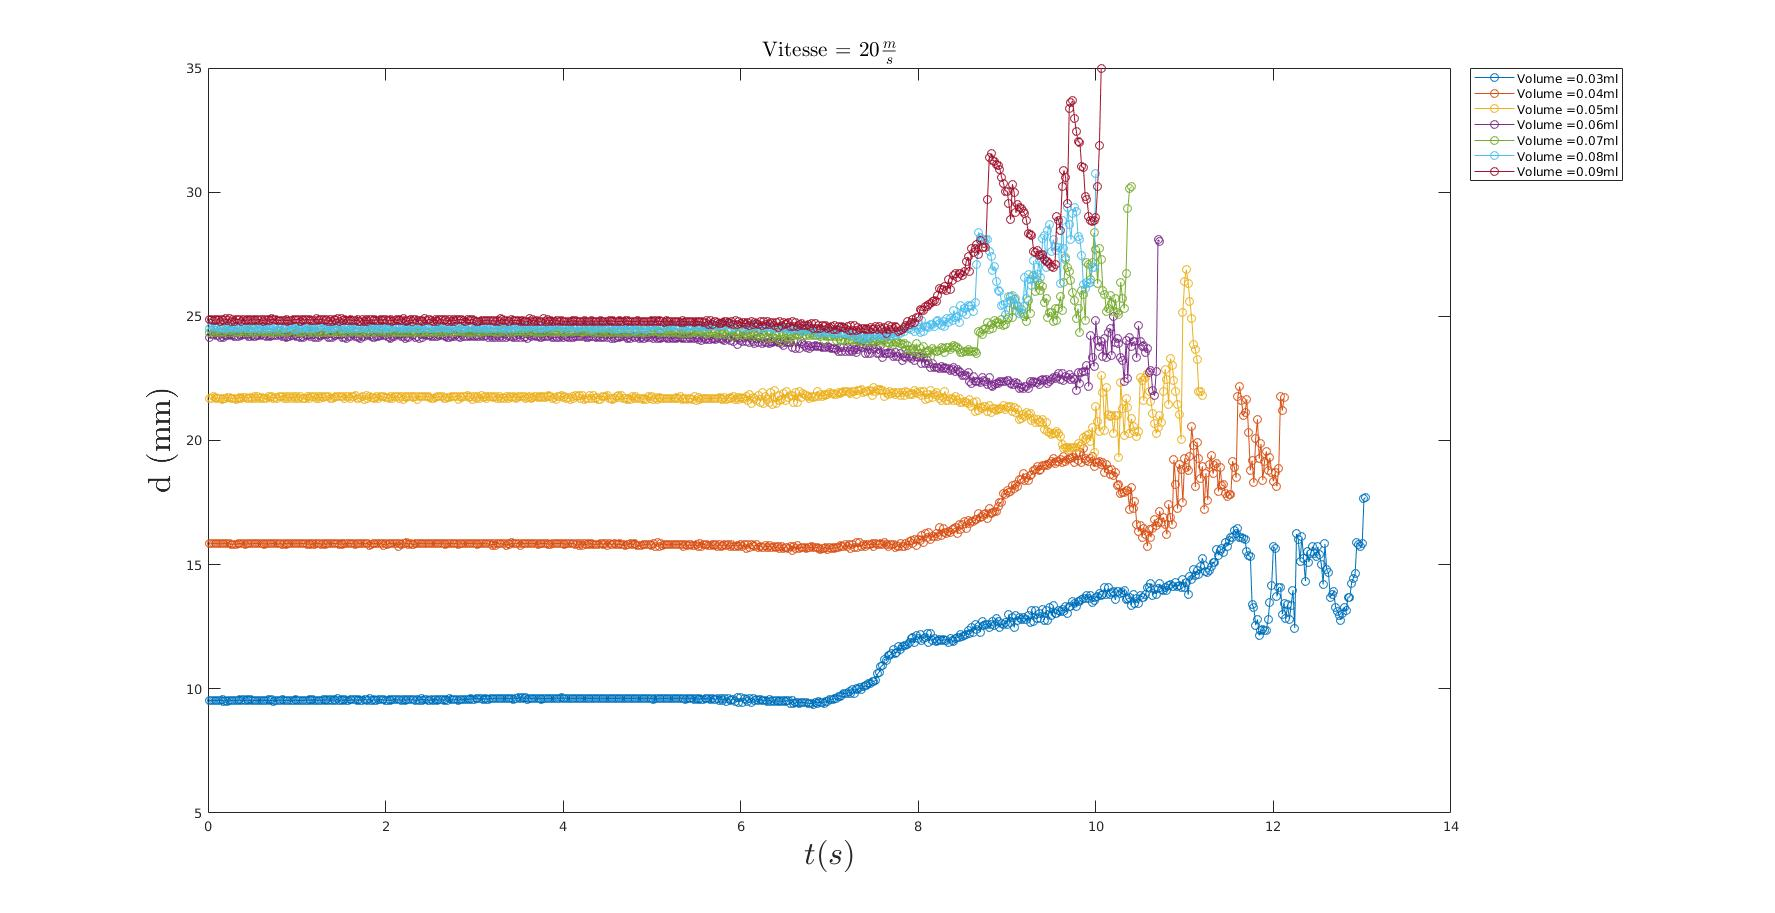
\includegraphics[width = \linewidth]{./gfx/v=20d.jpg}
	\caption{$d$, $U_{\infty}=20m.s^{-1}$}
		\label{fig:v=20d}
	\end{minipage}
	\begin{minipage}{0.7\linewidth}
	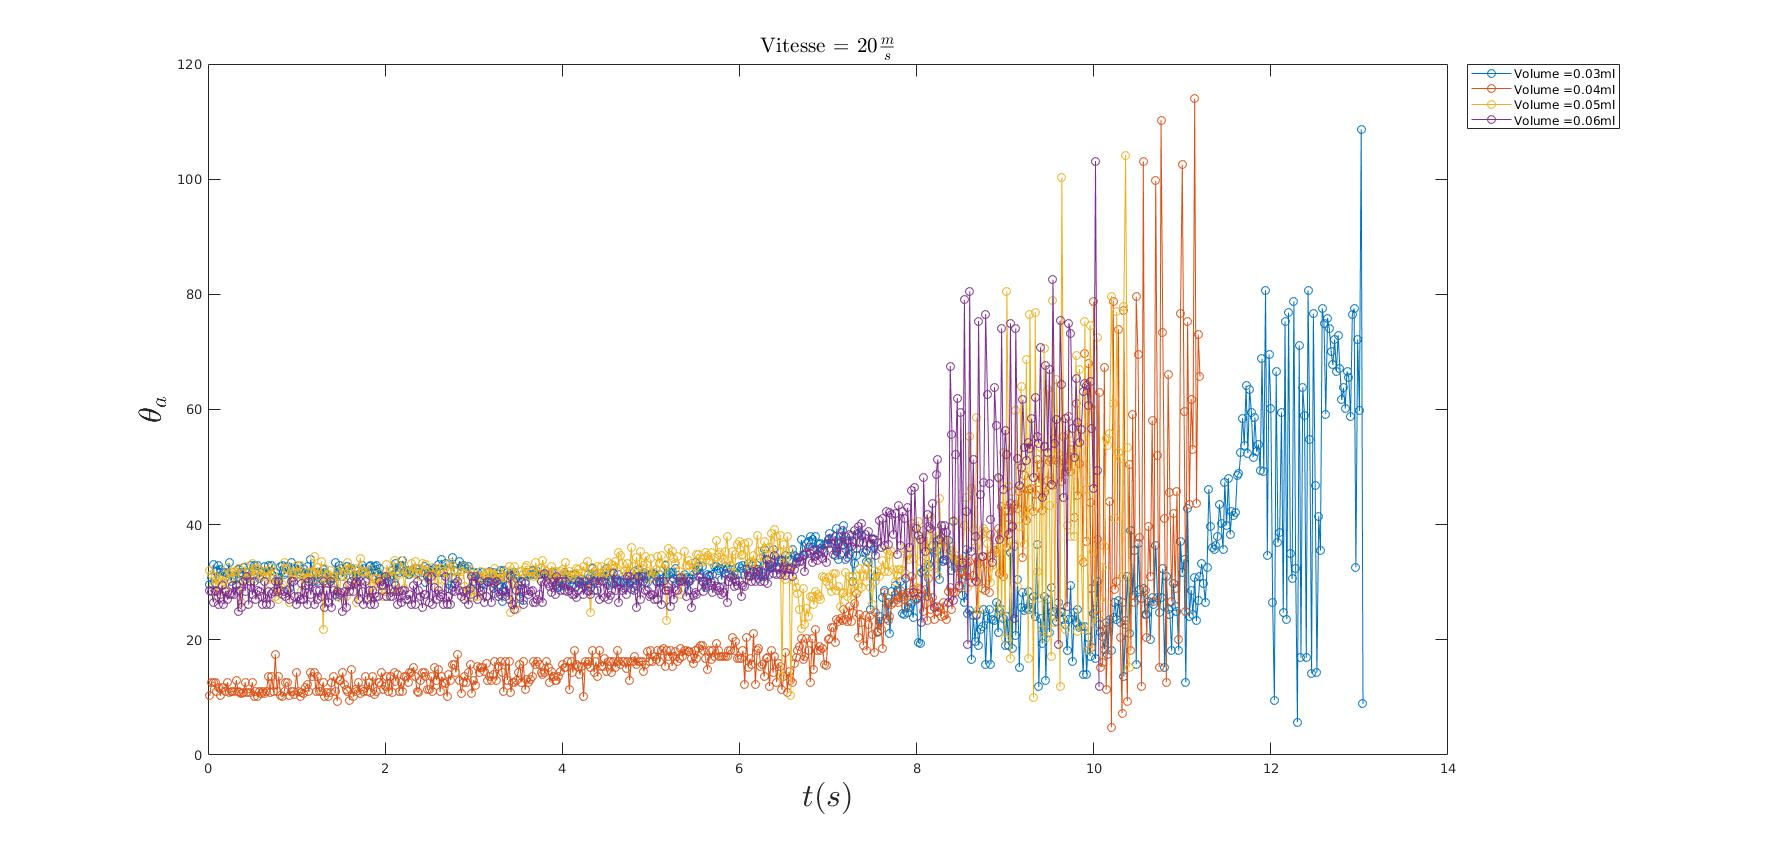
\includegraphics[width = \linewidth]{./gfx/v=20oa_2.jpg}
	\caption{$\theta_{a}$, $U_{\infty}=20m.s^{-1}$}
		\label{fig:v=20oa_2}
	\end{minipage}
	\begin{minipage}{0.75\linewidth}
	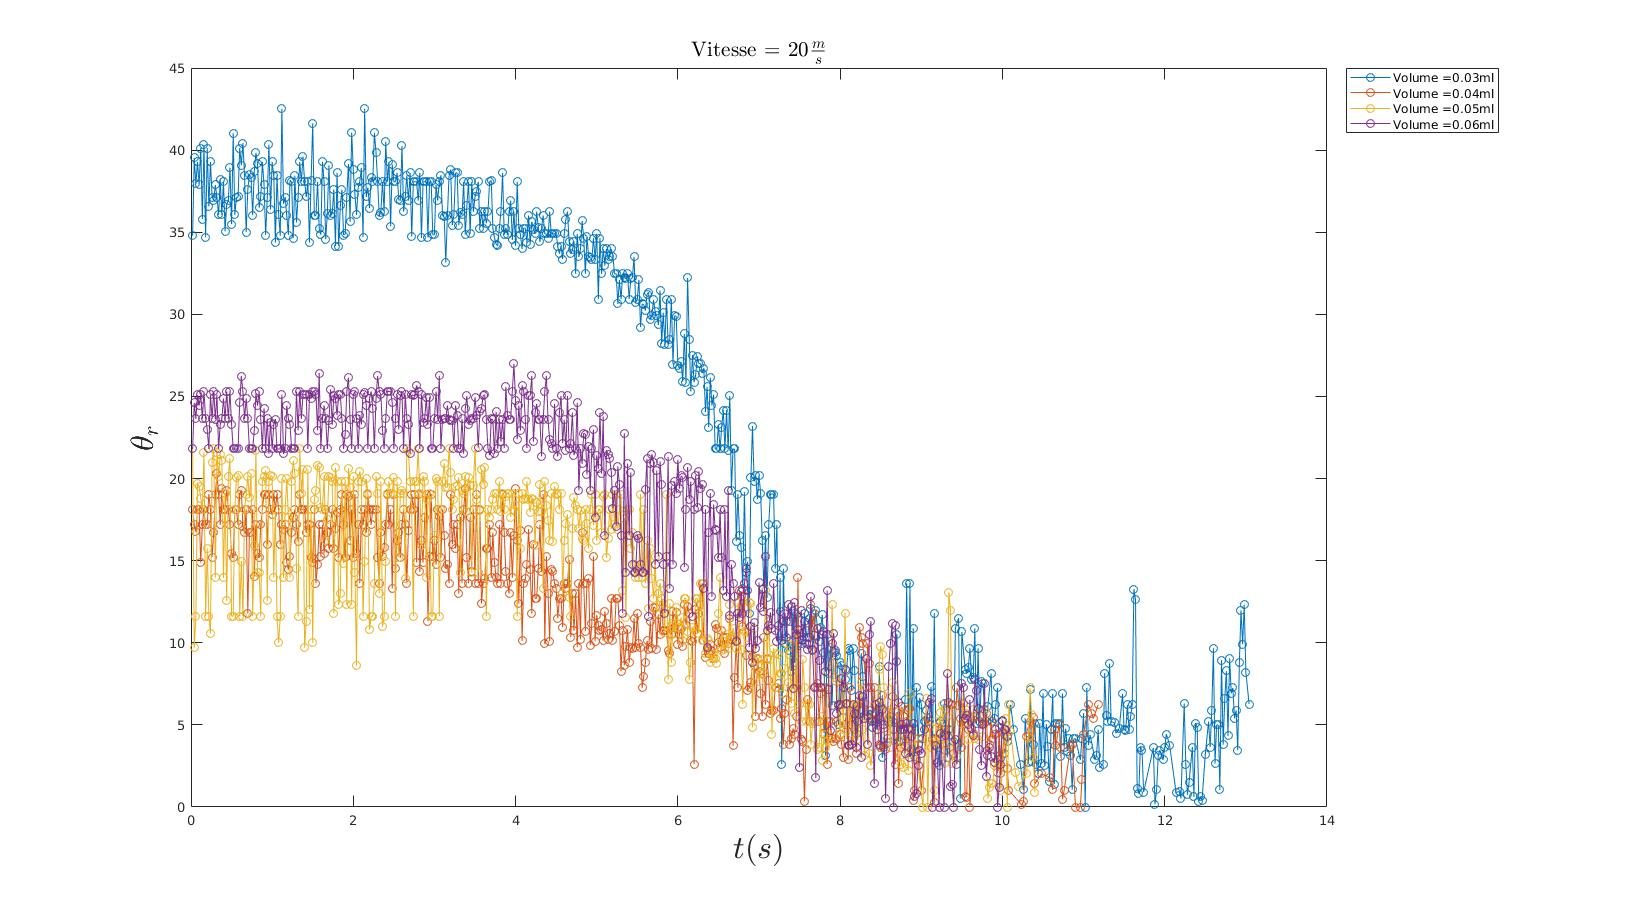
\includegraphics[width = \linewidth]{./gfx/v=20or_2.jpg}
	\caption{$\theta_{r}$, $U_{\infty}=20m.s^{-1}$}
		\label{fig:v=20or_2}
	\end{minipage}
\end{figure}


\begin{figure}[!h]
	\centering
	\begin{minipage}{0.7\linewidth}
	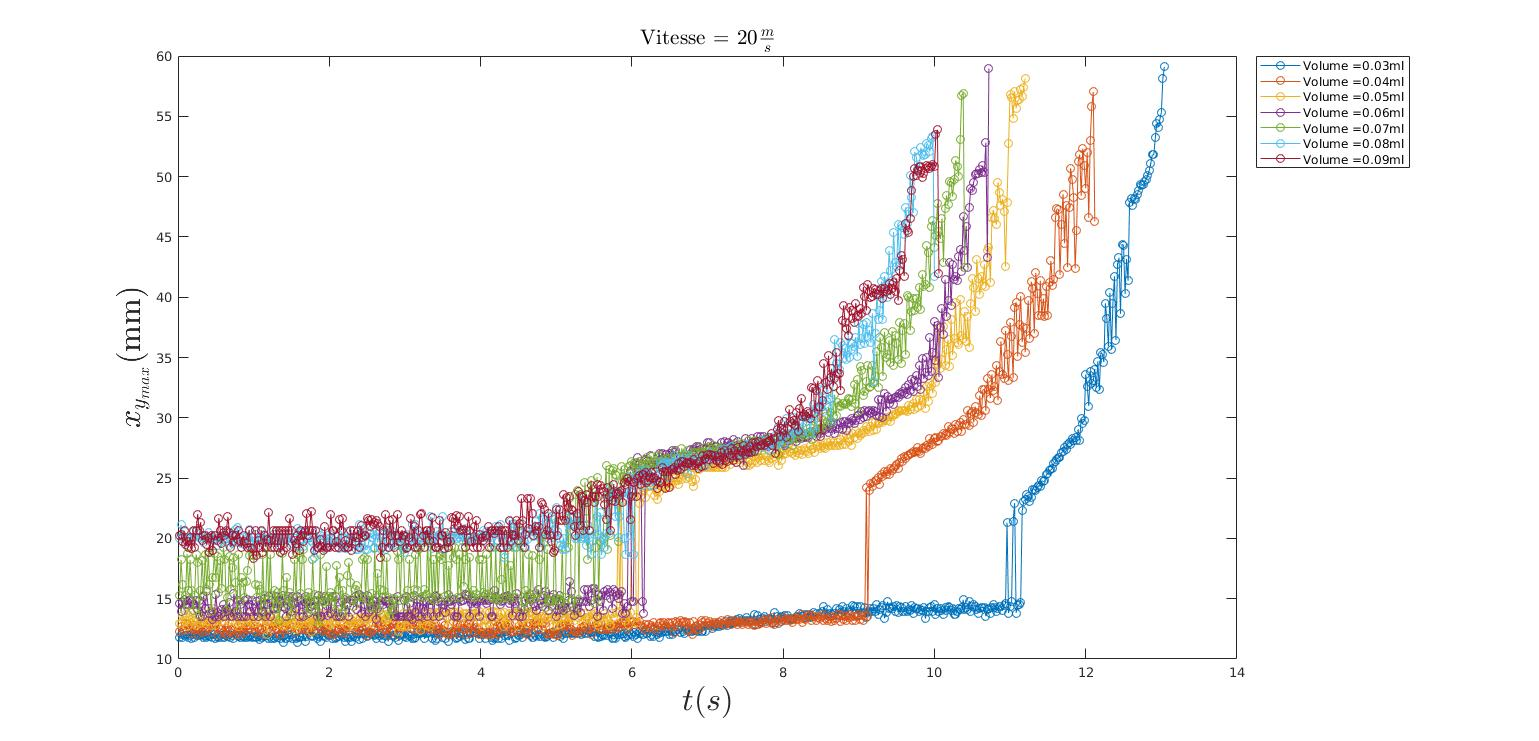
\includegraphics[width = \linewidth]{./gfx/v=20xm.jpg}
	\caption{$x_{max}$, $U_{\infty}=20m.s^{-1}$}
		\label{fig:v=20xm}
	\end{minipage}
	\begin{minipage}{0.7\linewidth}
	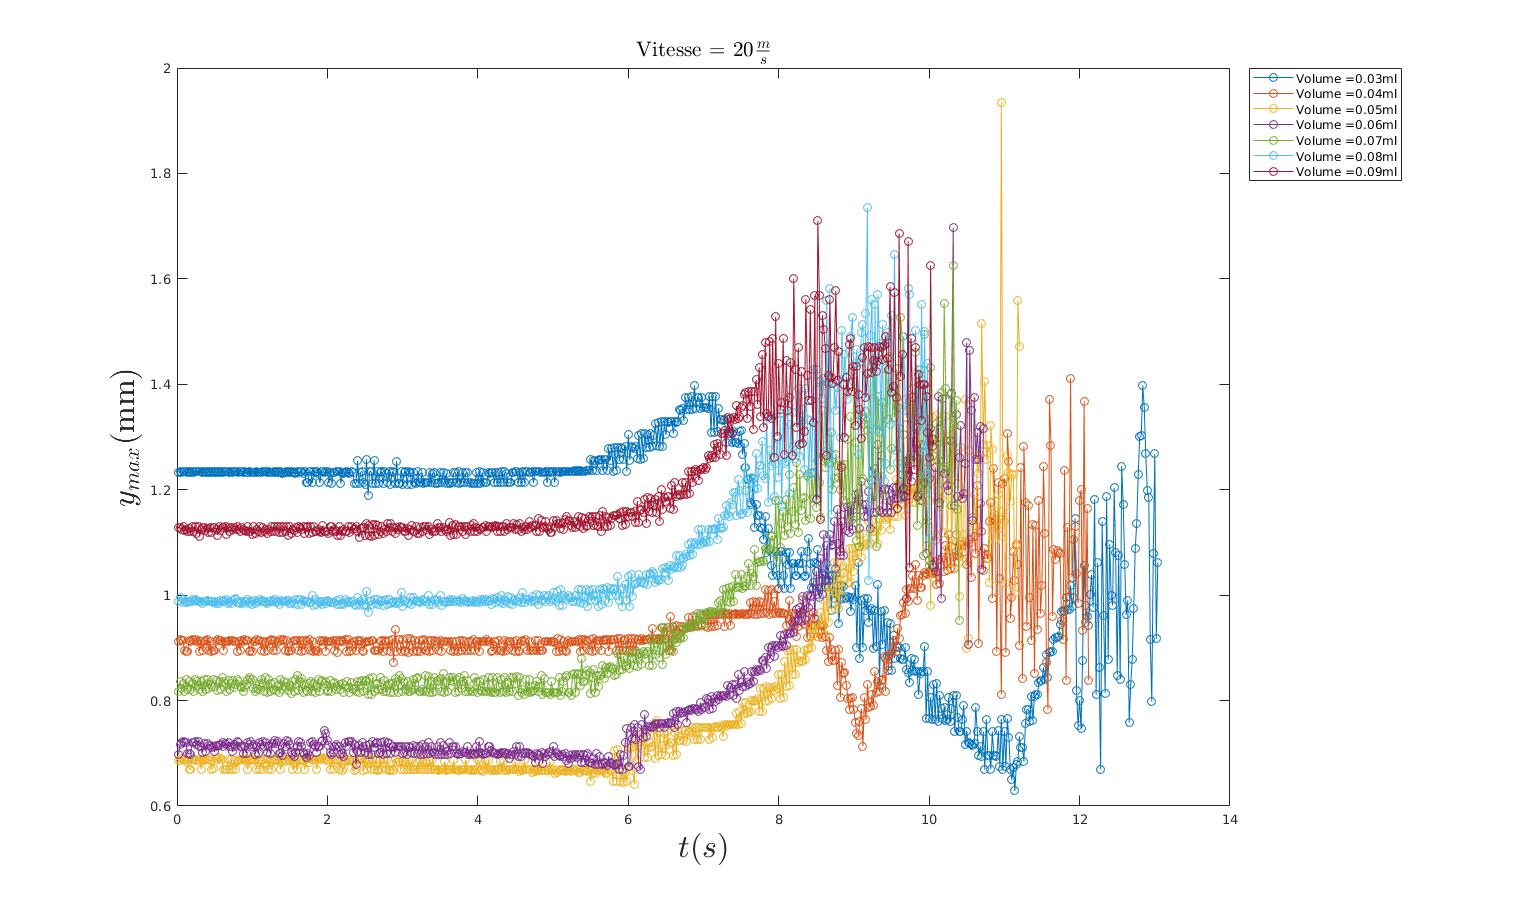
\includegraphics[width = \linewidth]{./gfx/v=20ym.jpg}
	\caption{$y_{max}$, $U_{\infty}=20m.s^{-1}$}
		\label{fig:v=20ym}
	\end{minipage}
\end{figure}

\newpage

\subsection{Vitesse de $24m.s^{-1}$}

Nous constatons aussi sur les figures \ref{fig:v=24d}, \ref{fig:v=24oa_2} et \ref{fig:v=24or_2} que $d$ reste constant un certain temps puis augmente ou diminue et $d$ se met à osciller s'il atteint une certaine longueur en augmentant.

L'angle $\theta_{a}$ lui aussi est d'abord constant, puis il augmente et se met à osciller autour de $\ang{50}$.

L'angle $\theta_{r}$ reste aussi constant un certain temps avant de diminuer et d'osciller autour de $\ang{5}$.

Nous observons aussi que la hauteur maximale de la goutte $y_{max}$, après une phase initiale où elle est presque constante, elle peut se mettre à baiser ou à augmenter, mais lorsque $y_{max}$ augmente et atteint une certaine hauteur, $y_{max}$ se met à osciller autour de cette hauteur.
\newpage
\begin{figure}[!h]
	\begin{minipage}{0.7\linewidth}
	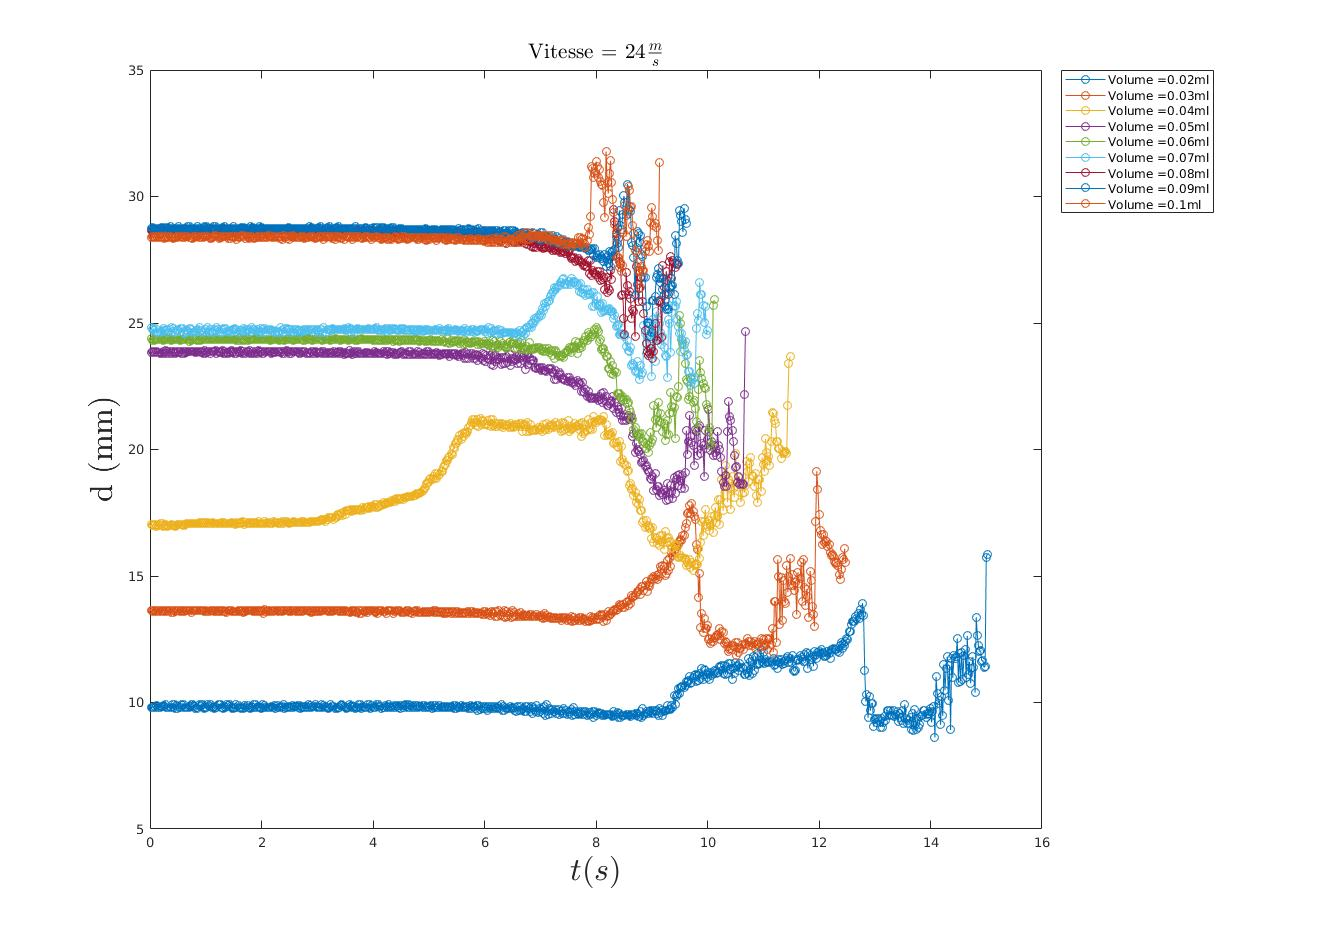
\includegraphics[width = \linewidth]{./gfx/v=24d.jpg}
	\caption{$d$, $U_{\infty}=24m.s^{-1}$}
		\label{fig:v=24d}
	\end{minipage}
	\begin{minipage}{0.7\linewidth}
	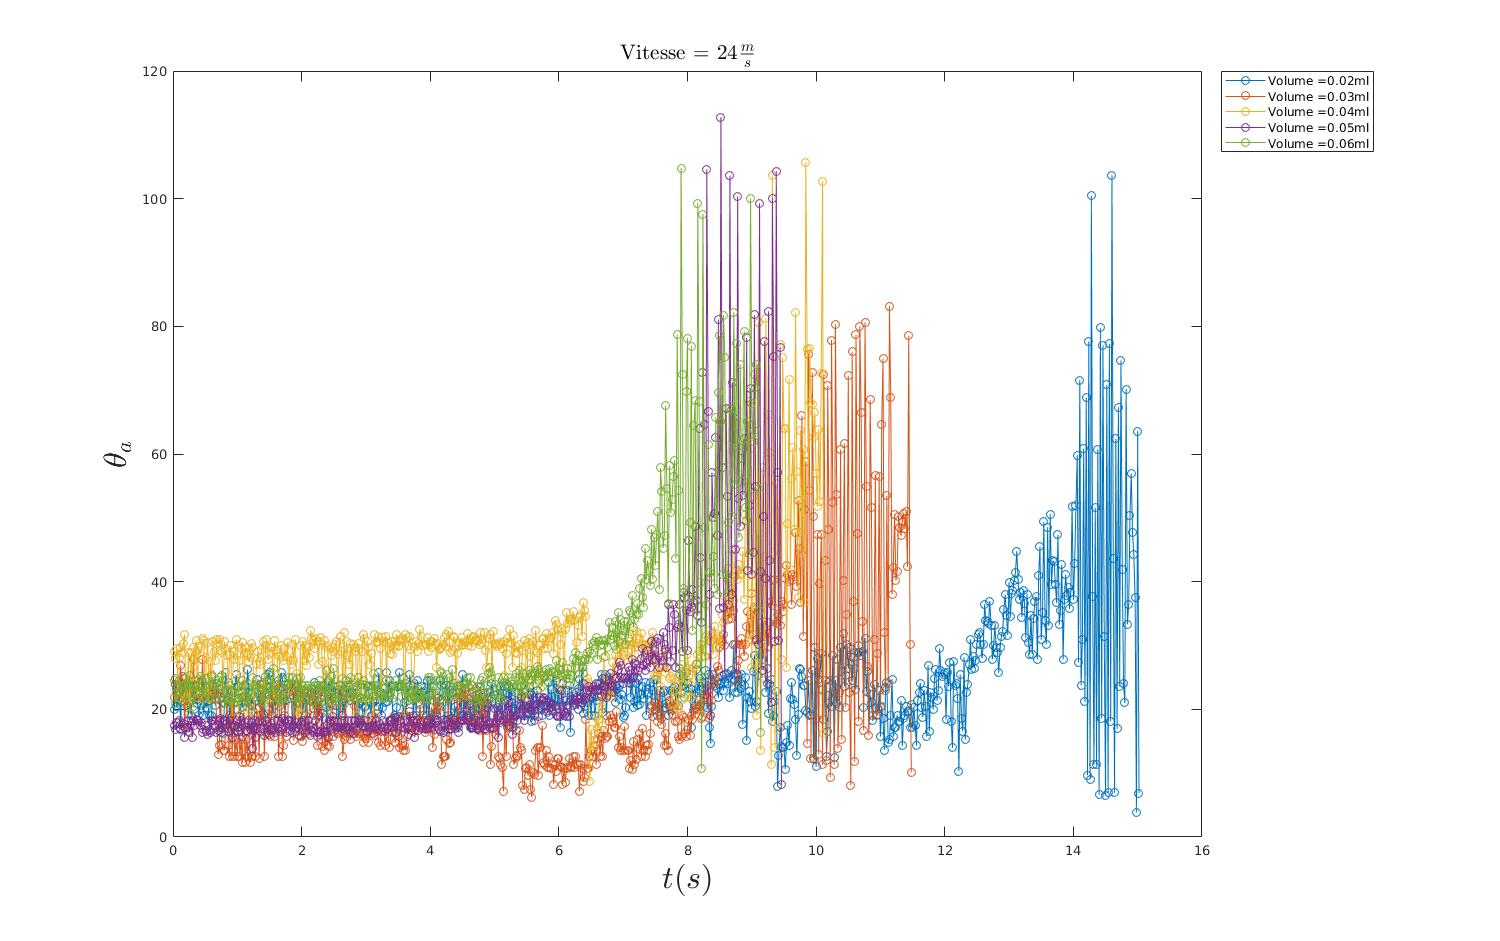
\includegraphics[width = \linewidth]{./gfx/v=24oa_2.jpg}
	\caption{$\theta_{a}$, $U_{\infty}=24m.s^{-1}$}
		\label{fig:v=24oa_2}
	\end{minipage}
	\begin{minipage}{0.7\linewidth}
	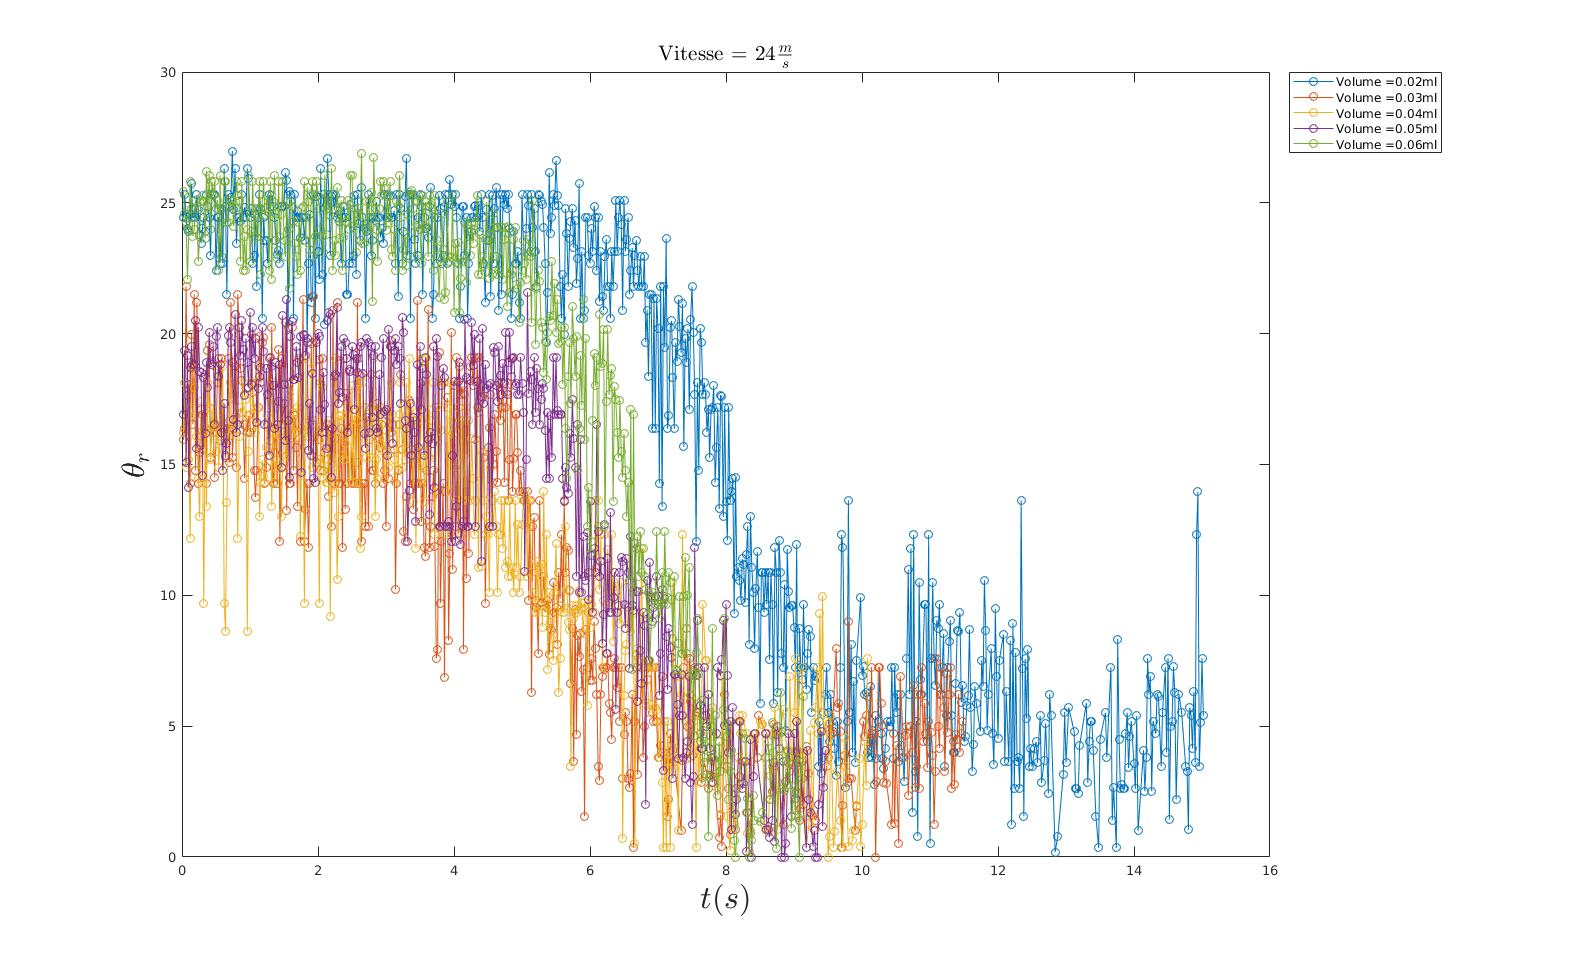
\includegraphics[width = \linewidth]{./gfx/v=24or_2.jpg}
	\caption{$\theta_{r}$, $U_{\infty}=24m.s^{-1}$}
		\label{fig:v=24or_2}
	\end{minipage}
\end{figure}

\begin{figure}[!h]
	\centering
	\begin{minipage}{0.7\linewidth}
	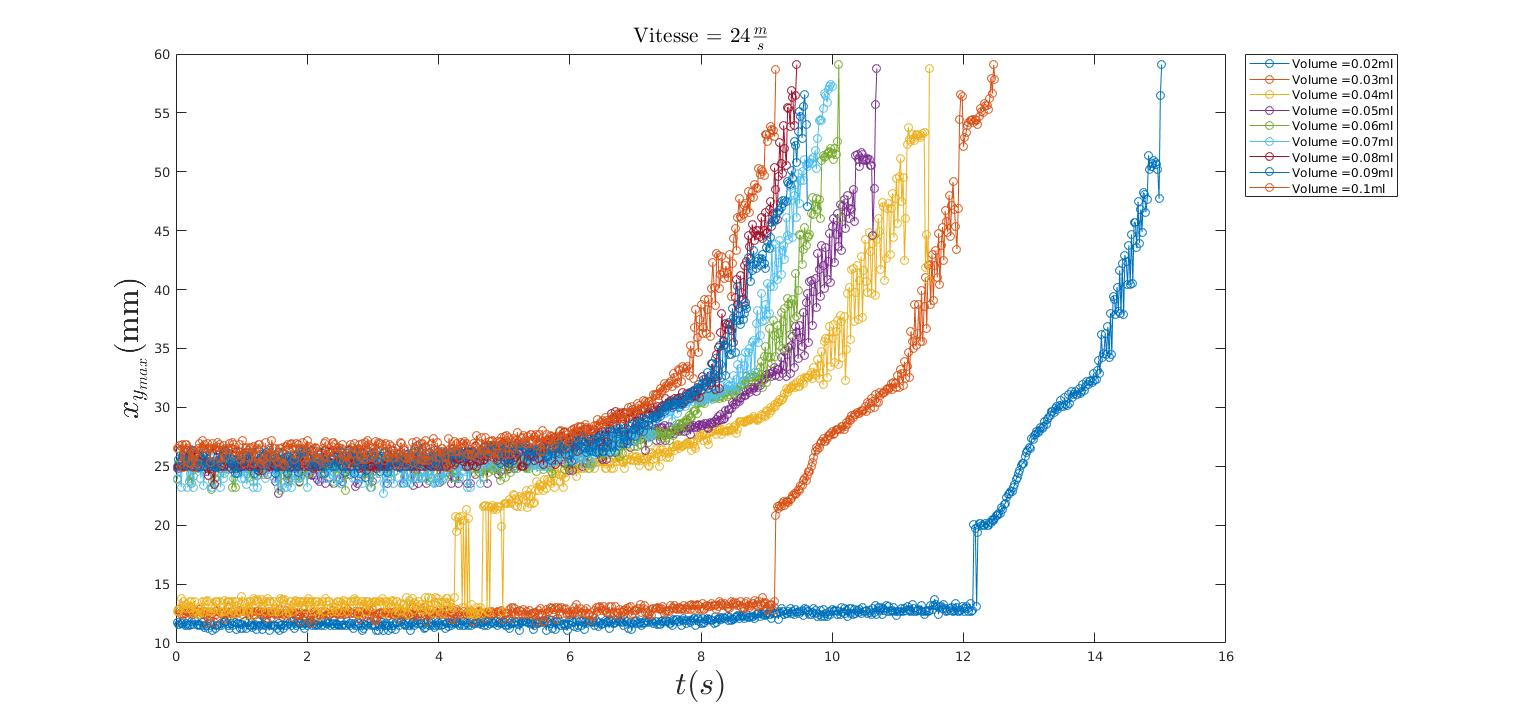
\includegraphics[width = \linewidth]{./gfx/v=24xm.jpg}
	\caption{$x_{max}$, $U_{\infty}=24m.s^{-1}$}
		\label{fig:v=24xm}
	\end{minipage}
	\begin{minipage}{0.7\linewidth}
	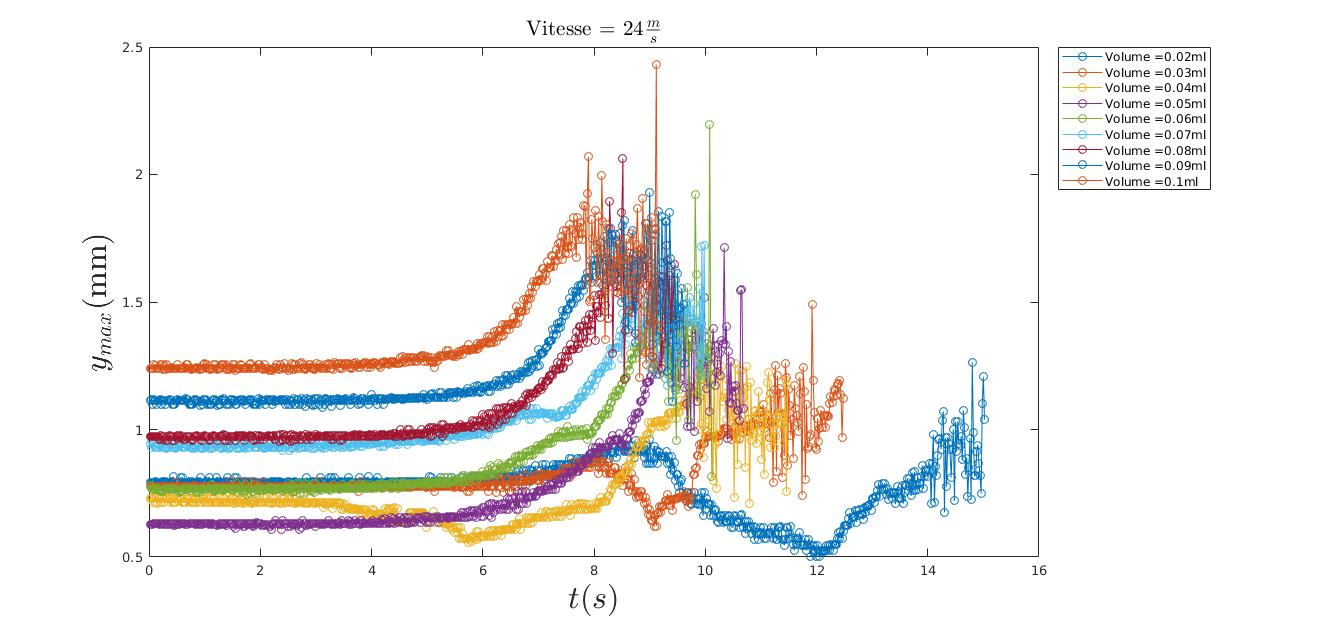
\includegraphics[width = \linewidth]{./gfx/v=24ym.jpg}
	\caption{$y_{max}$, $U_{\infty}=24m.s^{-1}$}
	\end{minipage}
		\label{fig:v=24ym}
\end{figure}

\subsection{Vitesse de $28m.s^{-1}$}
Nous constatons de même sur les figures \ref{fig:v=28d}, \ref{fig:v=28oa_2} et \ref{fig:v=28or_2} que $d$ reste constant un certain temps puis augmente ou diminue et $d$ se met à osciller s'il atteint une certaine longueur en augmentant.

L'angle $\theta_{a}$ lui aussi est d'abord constant, puis il augmente et se met à osciller autour de $\ang{50}$.

L'angle $\theta_{r}$ reste aussi constant un certain temps avant de diminuer et d'osciller autour de $\ang{5}$.

Nous observons aussi que la hauteur maximale de la goutte $y_{max}$, après une phase initiale où elle est presque constante, elle peut se mettre à baiser ou à augmenter, mais lorsque $y_{max}$ augmente et atteint une certaine hauteur, $y_{max}$ se met à osciller autour de cette hauteur.

\newpage
\begin{figure}[!ht]
	\begin{minipage}{0.7\linewidth}
	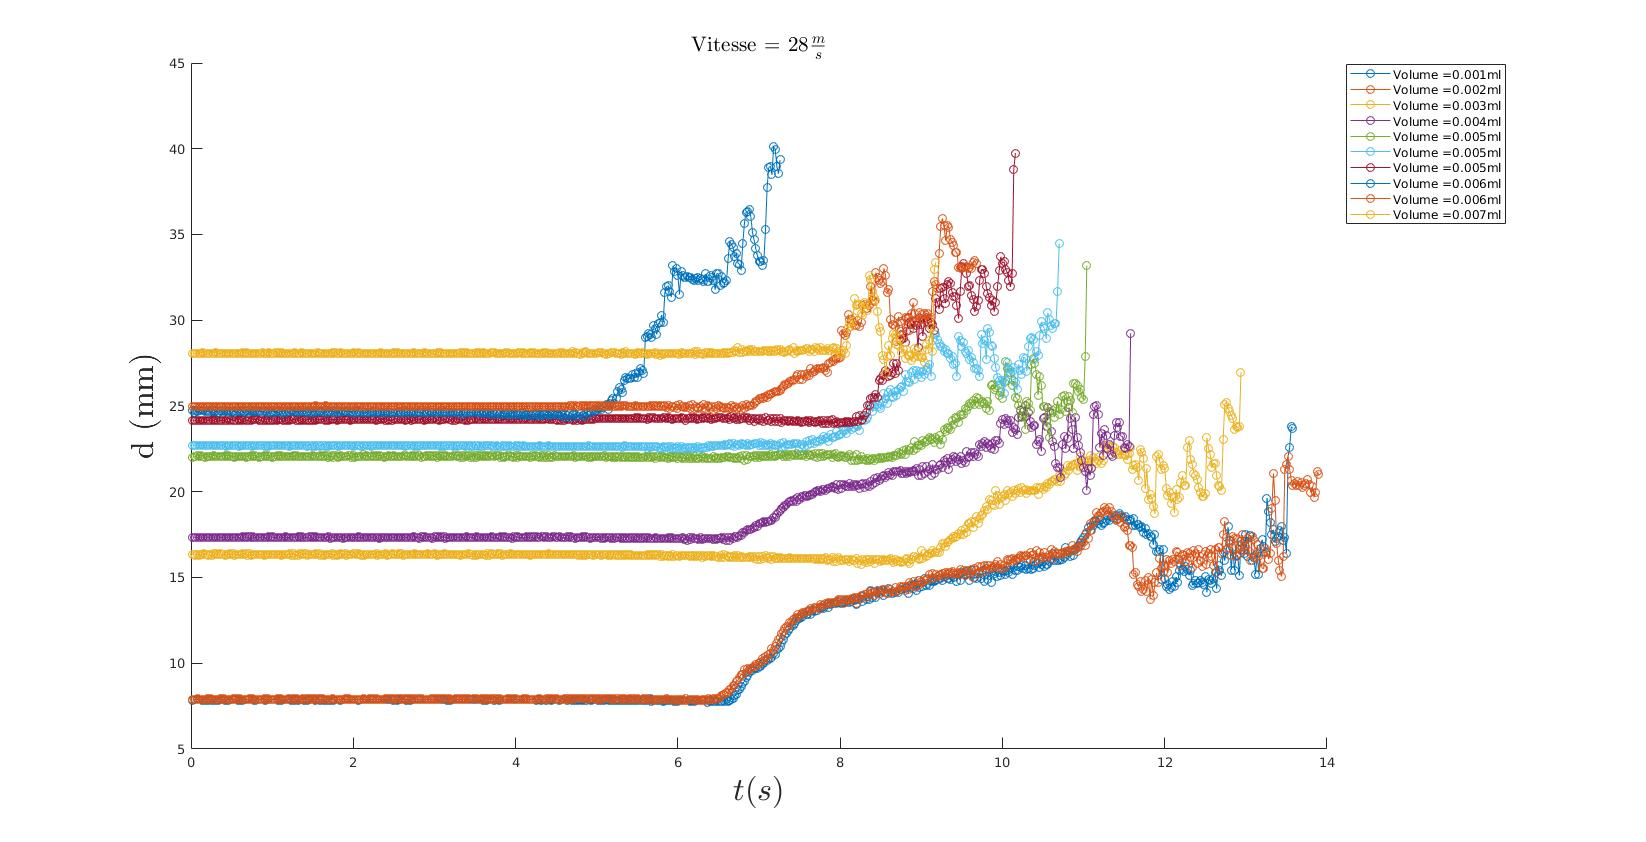
\includegraphics[width = \linewidth]{./gfx/v=28d.jpg}
	\caption{$d$, $U_{\infty}=28m.s^{-1}$}
		\label{fig:v=28d}
	\end{minipage}
	\begin{minipage}{0.7\linewidth}
	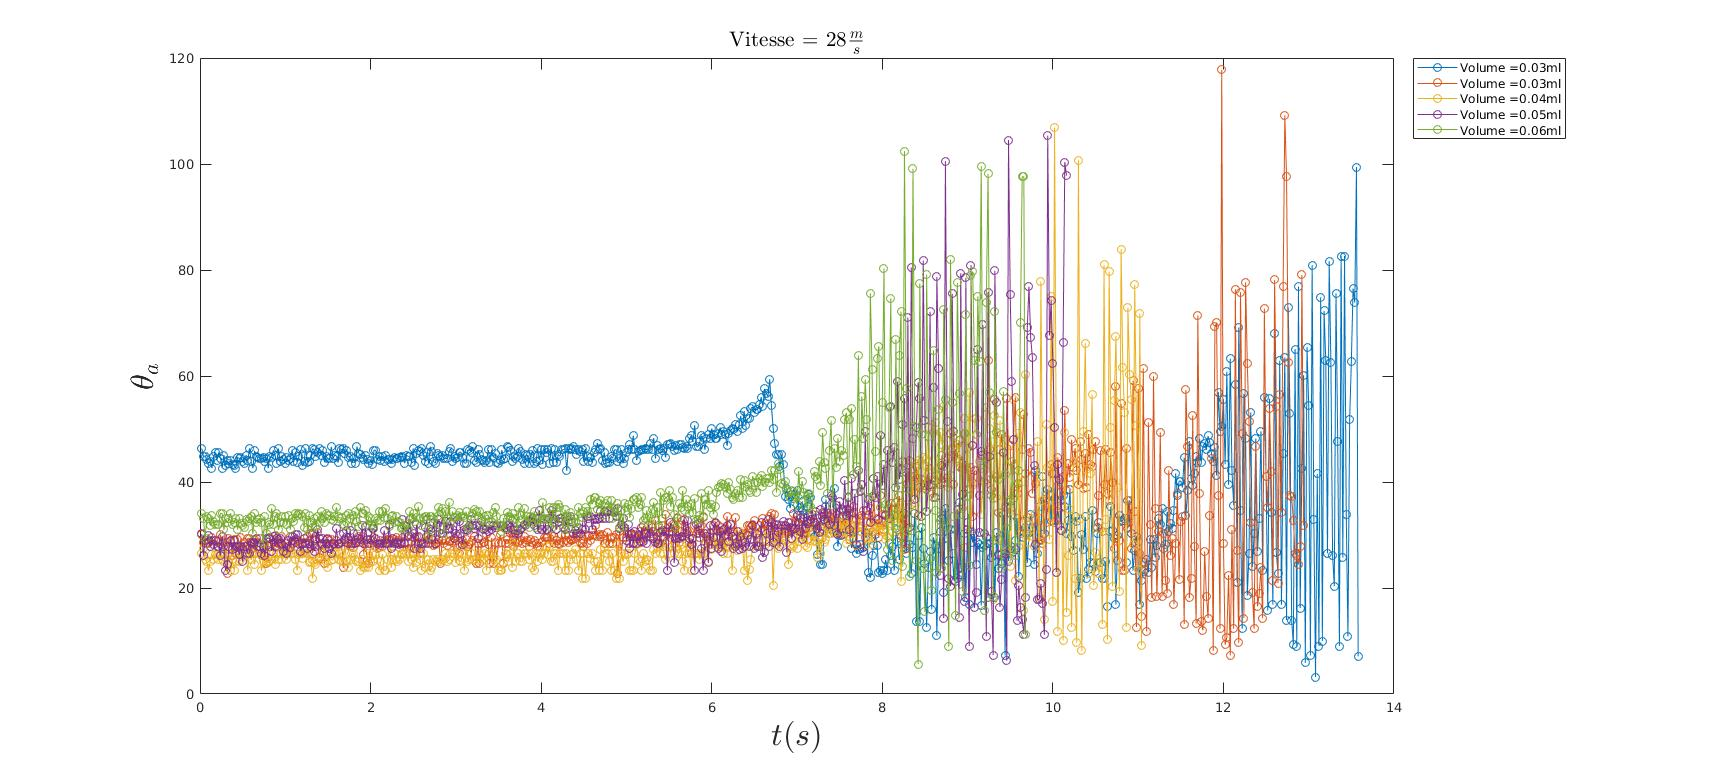
\includegraphics[width = \linewidth]{./gfx/v=28oa_2.jpg}
	\caption{$\theta_{a}$, $U_{\infty}=28m.s^{-1}$}
		\label{fig:v=28oa_2}
	\end{minipage}
	\begin{minipage}{0.7\linewidth}
	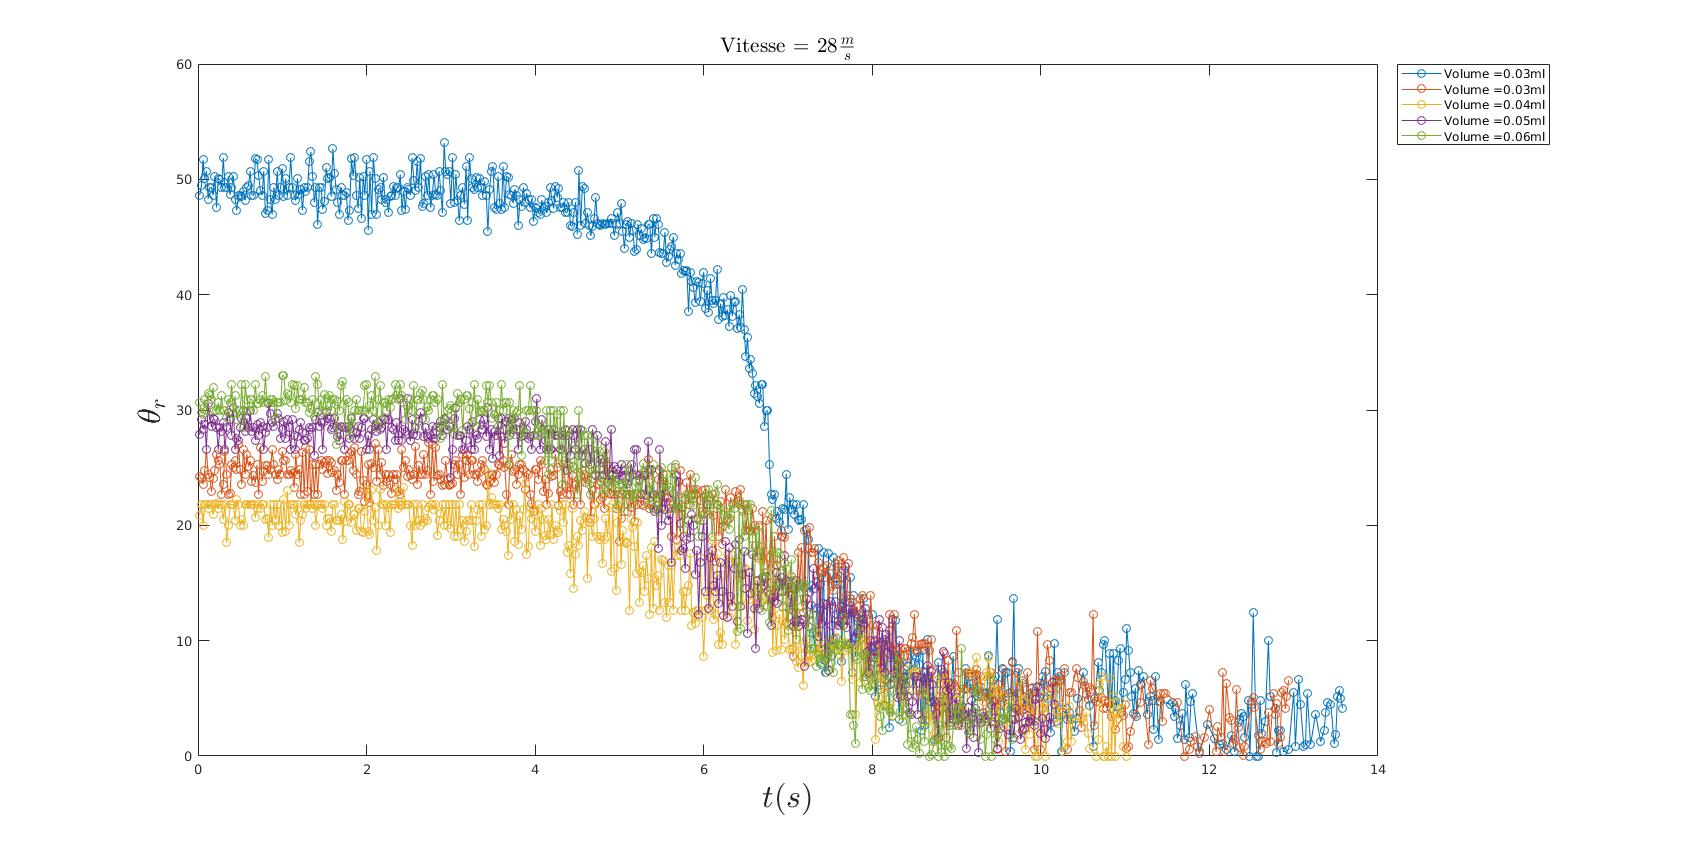
\includegraphics[width = \linewidth]{./gfx/v=28or_2.jpg}
	\caption{$\theta_{r}$, $U_{\infty}=28m.s^{-1}$}
		\label{fig:v=28or_2}
	\end{minipage}
\end{figure}

\newpage
\begin{figure}[!ht]
	\centering
	\begin{minipage}{0.7\linewidth}
	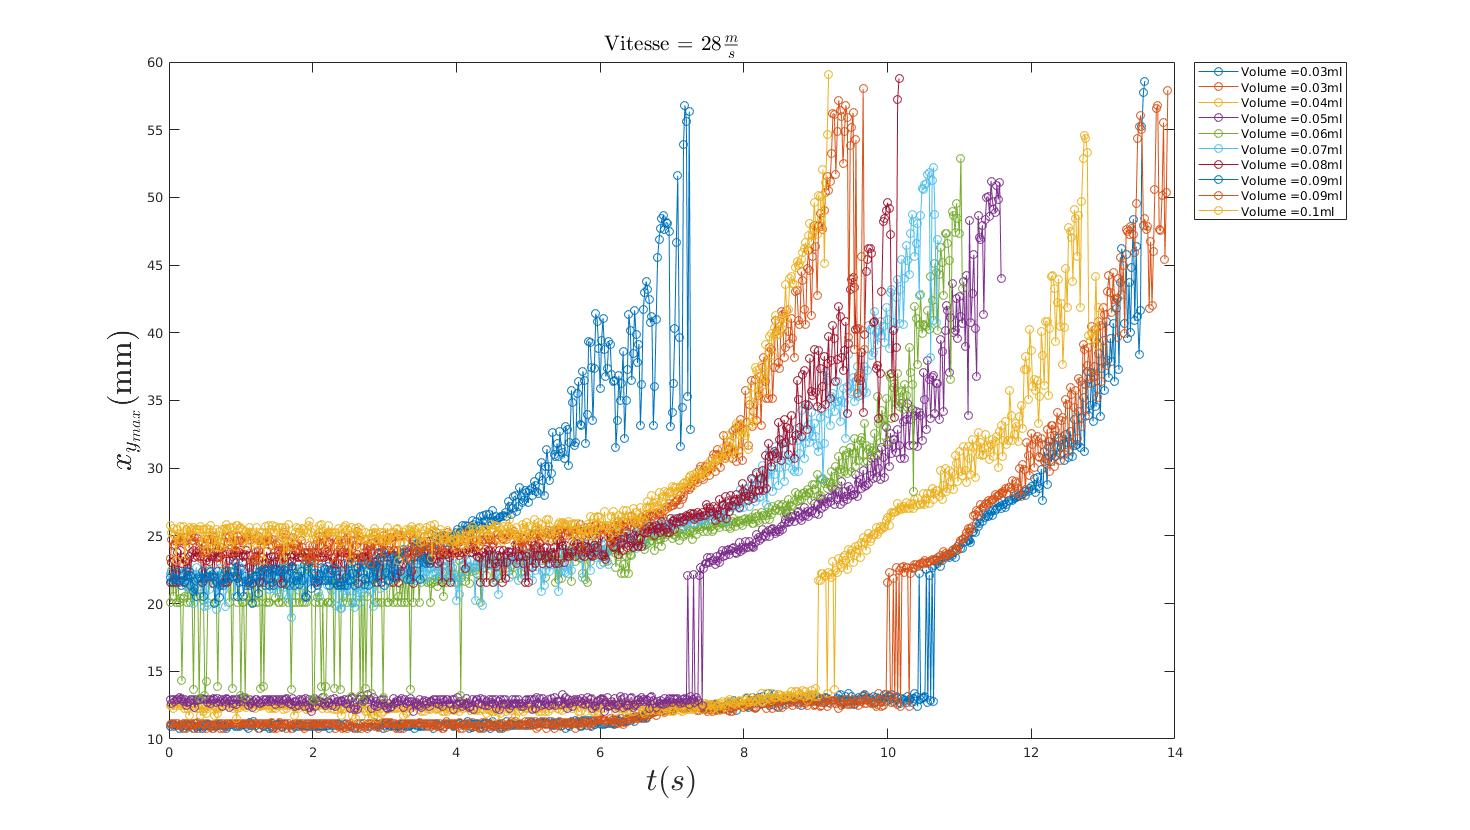
\includegraphics[width = \linewidth]{./gfx/v=28xm.jpg}
	\caption{$x_{max}$, $U_{\infty}=28m.s^{-1}$}
		\label{fig:v=28xm}
	\end{minipage}
	\begin{minipage}{0.7\linewidth}
	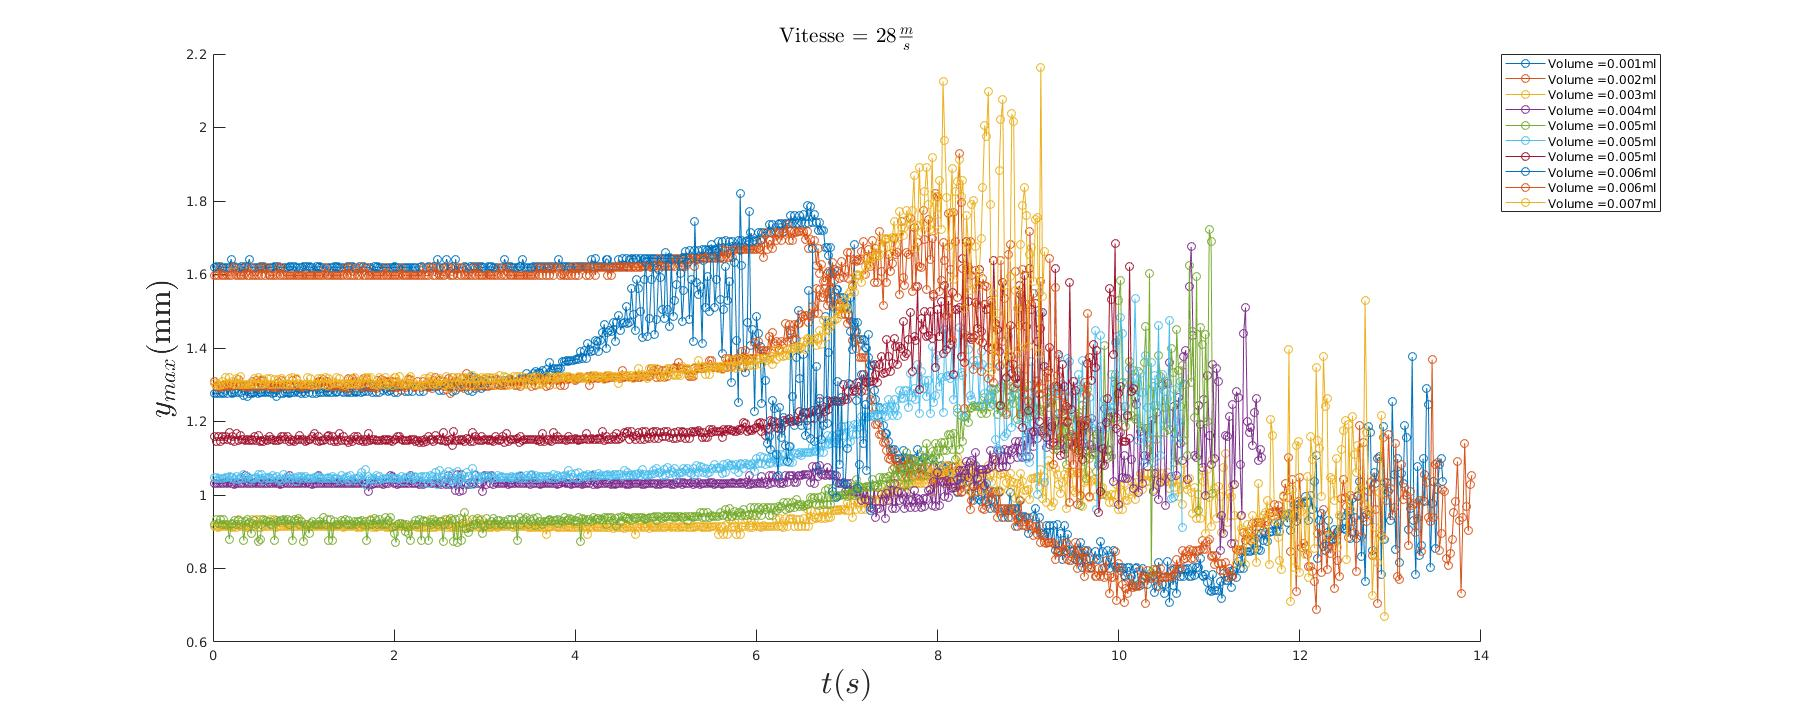
\includegraphics[width = \linewidth]{./gfx/v=28ym.jpg}
	\caption{$y_{max}$, $U_{\infty}=28m.s^{-1}$}
		\label{fig:v=28ym}
	\end{minipage}
\end{figure}

\subsection{Longueur $d$ à une vitesse de $24m.s^{-1}$ avec ou sans débit}

Nous présentons des mesures faites en injectant un volume de $0.06ml$ d'eau  à un debit fixé avec une vitesse dans la soufflerie déjà établie à environ $24m.s^{-1}$.

Nous comparons ces données avec une goutte de débit nulle qui a été formée sur notre surface lorsque la soufllerie était à l'arrêt et la soufflerie a été mise en marche pour obtenir la vitesse de $24m.s^{-1}$.\\


Nous observons sur la figure \ref{fig:p=365_vol=006d} que pour des débits non nuls la longueur $d$ augmente de plus en plus rapidement lorsque le débit augmente puis se met à osciller autour de la longueur pour laquelle on a un débit nul.

\begin{figure}[!h]
	\centering
	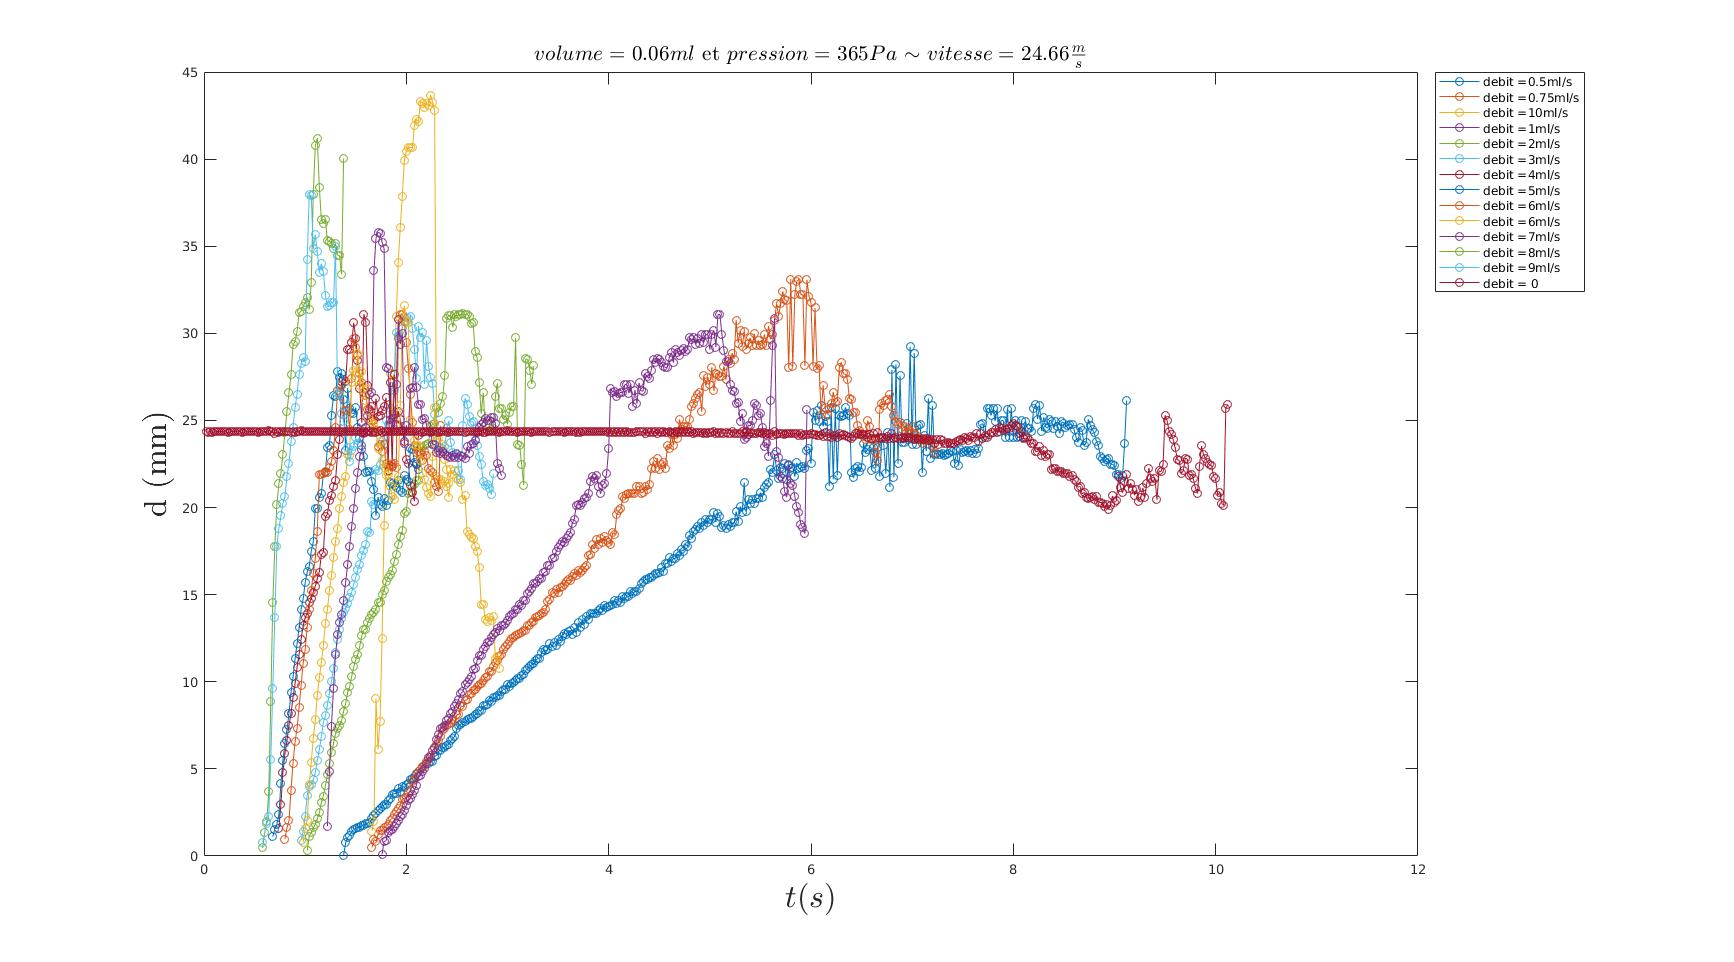
\includegraphics[width = \linewidth]{./gfx/p=365_vol=006d.jpg}
	\caption{$d$ , volume $= 0.06ml$, vitesse $\approx 24.7m.s^{-1}$}
\label{fig:p=365_vol=006d}
\end{figure}

%************************************************
\chapter{Conclusion}\label{ch:conclusion}
%************************************************

Nous avons fait l'étude d'une goutte d'eau sur une plaque plane en présence d'un écoulement.\\

Nous avons pris les photos de gouttes d'eau dans une soufflerie soit en injectant une goutte de volume donné (avec un certain débit) quand la vitesse était déjà établie dans la soufflerie, soit en injectant d'abord la goutte d'eau de volume donné avant de mettre la soufflerie en marche.

Les photos des gouttes d'eau ont été prises avec une caméra à la fréquence de $50Hz$, l'extraction des données de nos images a été faite à l'aide de Matlab et nous avons fait une analyse de nos résultats.\\


Pour affiner nos résultats, nous devons améliorer notre algorithme de détection (automatique pour des milliers d'images) des tangentes qui reste très sensible au nombre de points pris pour trouver la tangente.

Nous avons constaté que contrairement à ce qui se passe lorsqu'une goutte glisse sur un plan incliné, 
la goutte d'eau sur notre plaque (en présence d'un écoulement) oscillait autour d'une position (reculait et avançait) avant d'avancer subitement.

Ne nous attendions pas à voir ces oscillations et n'avons pas eu le temps de les étudier et cette étude devrait permettre d'améliorer nos résultats et de mieux comprendre le phénomène de goutte soufflée.

Nous filmions nos gouttes à une fréquence de $f_{exp} = 50Hz$ et il faudrait filmer avec le double de la fréquence la plus rapide $f_{max}$ d'oscillation d'une goutte dans nos expériences  pour étudier ces oscillations d'après le théorème de Shannon.

Si $f_{max} <= 25 Hz$, nos données pourront être utilisées pour faire l'étude de ces oscillations.


Changer les conditions de mouillage en changeant le liquide ou de plaque plane. Nous avons fait nos expériences uniquement avec de l'eau pour liquide sur une plaque plane en acier. \\

Ce stage nous a permis de nous initier à la recherche.

La partie expérimentale du stage nous a  permis d'apprendre à mesurer des profils de couche limite (avec l'anémomètre à fil chaud), de passer du temps à utiliser une soufflerie, d'apprendre à utiliser une caméra et de découvrir plein d'autres instruments.

La partie numérique du stage nous a permis de découvrir le traitement d'image et pour moi c'est un acquis inestimable.
%\include{multiToC} % <--- just debug stuff, ignore for your documents
% ********************************************************************
% Backmatter
%*******************************************************
%\appendix
%\renewcommand{\thechapter}{\alph{chapter}}
%\cleardoublepage
%\part{Appendix}
%%********************************************************************
% Appendix
%*******************************************************
% If problems with the headers: get headings in appendix etc. right
%\markboth{\spacedlowsmallcaps{Appendix}}{\spacedlowsmallcaps{Appendix}}
\chapter{Appendix Test}
Lorem ipsum at nusquam appellantur his, ut eos erant homero
concludaturque. Albucius appellantur deterruisset id eam, vivendum
partiendo dissentiet ei ius. Vis melius facilisis ea, sea id convenire
referrentur, takimata adolescens ex duo. Ei harum argumentum per. Eam
vidit exerci appetere ad, ut vel zzril intellegam interpretaris.
\graffito{More dummy text.}

%Errem omnium ea per, pro congue populo ornatus cu, ex qui dicant
%nemore melius. No pri diam iriure euismod. Graecis eleifend
%appellantur quo id. Id corpora inimicus nam, facer nonummy ne pro,
%kasd repudiandae ei mei. Mea menandri mediocrem dissentiet cu, ex
%nominati imperdiet nec, sea odio duis vocent ei. Tempor everti
%appareat cu ius, ridens audiam an qui, aliquid admodum conceptam ne
%qui. Vis ea melius nostrum, mel alienum euripidis eu.

\section{Appendix Section Test}
Test: \autoref{tab:moreexample} (This reference should have a
lowercase, small caps \spacedlowsmallcaps{A} if the option
\texttt{floatperchapter} is activated, just as in the table itself
 $\rightarrow$ however, this does not work at the moment.)

\begin{table}[h]
    \myfloatalign
    \begin{tabularx}{\textwidth}{Xll} \toprule
        \tableheadline{labitur bonorum pri no} & \tableheadline{que vista}
        & \tableheadline{human} \\ \midrule
        fastidii ea ius & germano &  demonstratea \\
        suscipit instructior & titulo & personas \\
        %postulant quo & westeuropee & sanctificatec \\
        \midrule
        quaestio philosophia & facto & demonstrated \\
        %autem vulputate ex & parola & romanic \\
        %usu mucius iisque & studio & sanctificatef \\
        \bottomrule
    \end{tabularx}
    \caption[Autem usu id]{Autem usu id.}
    \label{tab:moreexample}
\end{table}

%Nulla fastidii ea ius, exerci suscipit instructior te nam, in ullum
%postulant quo. Congue quaestio philosophia his at, sea odio autem
%vulputate ex. Cu usu mucius iisque voluptua. Sit maiorum propriae at,
%ea cum primis intellegat. Hinc cotidieque reprehendunt eu nec. Autem
%timeam deleniti usu id, in nec nibh altera.




\section{Another Appendix Section Test}
Equidem detraxit cu nam, vix eu delenit periculis. Eos ut vero
constituto, no vidit propriae complectitur sea. Diceret nonummy in
has, no qui eligendi recteque consetetur. Mel eu dictas suscipiantur,
et sed placerat oporteat. At ipsum electram mei, ad aeque atomorum
mea. There is also a useless Pascal listing below: \autoref{lst:useless}.

\begin{lstlisting}[float=b,language=Pascal,frame=tb,caption={A floating example (\texttt{listings} manual)},label=lst:useless]
for i:=maxint downto 0 do
begin
{ do nothing }
end;
\end{lstlisting}

%Ei solet nemore consectetuer nam. Ad eam porro impetus, te choro omnes
%evertitur mel. Molestie conclusionemque vel at, no qui omittam
%expetenda efficiendi. Eu quo nobis offendit, verterem scriptorem ne
%vix.


%********************************************************************
% Other Stuff in the Back
%*******************************************************
%\cleardoublepage%********************************************************************
% Bibliography
%*******************************************************
% work-around to have small caps also here in the headline
% https://tex.stackexchange.com/questions/188126/wrong-header-in-bibliography-classicthesis
% Thanks to Enrico Gregorio
\defbibheading{bibintoc}[\bibname]{%
  \phantomsection
  \manualmark
  \markboth{\spacedlowsmallcaps{#1}}{\spacedlowsmallcaps{#1}}%
  \addtocontents{toc}{\protect\vspace{\beforebibskip}}%
  \addcontentsline{toc}{chapter}{\tocEntry{#1}}%
  \chapter*{#1}%
}
\printbibliography[heading=bibintoc]

% Old version, will be removed later
% work-around to have small caps also here in the headline
%\manualmark
%\markboth{\spacedlowsmallcaps{\bibname}}{\spacedlowsmallcaps{\bibname}} % work-around to have small caps also
%\phantomsection
%\refstepcounter{dummy}
%\addtocontents{toc}{\protect\vspace{\beforebibskip}} % to have the bib a bit from the rest in the toc
%\addcontentsline{toc}{chapter}{\tocEntry{\bibname}}
%\label{app:bibliography}
%\printbibliography

%\cleardoublepage%*******************************************************
% Declaration
%*******************************************************
\pdfbookmark[0]{Declaration}{declaration}
\chapter*{Declaration}
\thispagestyle{empty}
Put your declaration here.
\bigskip

\noindent\textit{\myLocation, \myTime}

\smallskip

\begin{flushright}
    \begin{tabular}{m{5cm}}
        \\ \hline
        \centering\myName \\
    \end{tabular}
\end{flushright}

%\cleardoublepage\pagestyle{empty}

\hfill

\vfill


\pdfbookmark[0]{Colophon}{colophon}
\section*{Colophon}
This document was typeset using the typographical look-and-feel \texttt{classicthesis} developed by Andr\'e Miede and Ivo Pletikosić.
The style was inspired by Robert Bringhurst's seminal book on typography ``\emph{The Elements of Typographic Style}''.
\texttt{classicthesis} is available for both \LaTeX\ and \mLyX:
\begin{center}
\url{https://bitbucket.org/amiede/classicthesis/}
\end{center}
Happy users of \texttt{classicthesis} usually send a real postcard to the author, a collection of postcards received so far is featured here:
\begin{center}
\url{http://postcards.miede.de/}
\end{center}
Thank you very much for your feedback and contribution.

\bigskip

\noindent\finalVersionString

%Hermann Zapf's \emph{Palatino} and \emph{Euler} type faces (Type~1 PostScript fonts \emph{URW
%Palladio L} and \emph{FPL}) are used. The ``typewriter'' text is typeset in \emph{Bera Mono},
%originally developed by Bitstream, Inc. as ``Bitstream Vera''. (Type~1 PostScript fonts were made
%available by Malte Rosenau and
%Ulrich Dirr.)

%\paragraph{note:} The custom size of the textblock was calculated
%using the directions given by Mr. Bringhurst (pages 26--29 and
%175/176). 10~pt Palatino needs  133.21~pt for the string
%``abcdefghijklmnopqrstuvwxyz''. This yields a good line length between
%24--26~pc (288--312~pt). Using a ``\emph{double square textblock}''
%with a 1:2 ratio this results in a textblock of 312:624~pt (which
%includes the headline in this design). A good alternative would be the
%``\emph{golden section textblock}'' with a ratio of 1:1.62, here
%312:505.44~pt. For comparison, \texttt{DIV9} of the \texttt{typearea}
%package results in a line length of 389~pt (32.4~pc), which is by far
%too long. However, this information will only be of interest for
%hardcore pseudo-typographers like me.%
%
%To make your own calculations, use the following commands and look up
%the corresponding lengths in the book:
%\begin{verbatim}
%    \settowidth{\abcd}{abcdefghijklmnopqrstuvwxyz}
%    \the\abcd\ % prints the value of the length
%\end{verbatim}
%Please see the file \texttt{classicthesis.sty} for some precalculated
%values for Palatino and Minion.
%
%    \settowidth{\abcd}{abcdefghijklmnopqrstuvwxyz}
%    \the\abcd\ % prints the value of the length

% ********************************************************************
% Game Over: Restore, Restart, or Quit?
%*******************************************************
\addtocontents{toc}{\protect\vspace{\beforebibskip}} % to have the bib a bit from the rest in the toc
\addcontentsline{toc}{chapter}{\tocEntry{\bibname}}
\begin{thebibliography}{1}
   \bibitem{NOLWEN}
   NOLWEN LE GRAND, ADRIAN DAERR, LAURENT LIMAT,
          \emph{Shape and motion of drops sliding down an inclined plane},
          J. Fluid Mech.,
          2005.
 \bibitem{Gennes}
          De Gennes,
          \emph{Capillarity and Wetting Phenomena: Drops, Bubbles, Pearls, Waves},
          Springer-Verlag New York Inc.,
          2004.
      
\end{thebibliography}
\end{document}
% ********************************************************************
